%\documentclass[11pt,a4paper]{article}
\documentclass[11pt
  , a4paper
  , article
  , oneside
%  , twoside
%  , draft
]{memoir}

\usepackage{control}
\usepackage[numbers]{natbib}
\definecolor{babypink}{rgb}{0.96, 0.76, 0.76}
\definecolor{blizzardblue}{rgb}{0.67, 0.9, 0.93}

\begin{document}

\newcommand{\technumber}{
  RAON Control-Document Series\\
  Revision : v1.0,   Release : Jan. 02. 2015}
\title{\textbf{SNMP 이해 및 응답시간 테스트}}

\author{박미정\thanks{mijoy0909@ibs.re.kr} \\

  Rare Isotope Science Project\\
  Institute for Basic Science, Daejeon, South Korea
}
\date{\today}

\renewcommand{\maketitlehooka}{\begin{flushright}\textsf{\technumber}\end{flushright}}
%\renewcommand{\maketitlehookb}{\centering\textsf{\subtitle}}
%\renewcommand{\maketitlehookc}{C}
%\renewcommand{\maketitlehookd}{D}

\maketitle

\begin{abstract}
SNMP는 IP 네트워크에서 장치를 관리하기 위한 공식 인터넷 표준 프로토콜(Official Internet Standards Protocol)\citep{oisp}이다. 본 문서는 SNMP의 이해, SNMP를 이용한 장비 모니터링 결과 그리고 다양한 네트워크 환경에서 SNMP 버전 별 응답시간에 관한 테스트 결과에 대해 설명한다. 
\end{abstract}

\chapter{SNMP의 이해}
\section{SNMP란?}

SNMP(Simple Network Management Protocol)는 IP네트워크 상의 장치 및 장비들을 관리하고 모니터링하기 위한 인터넷 표준 프로토콜이다. SNMP는 Manager와 Agent로 구성되어있으며, Manager는 NMS(Network Management Stations)로 표현되기도 한다. Manager는 Agent에게 원하는 장비의 정보를 요청하며, 장비의 설정을 변경한다. Agent는 Manager가 요청한 장비의 정보를 제공하고, 시스템 충돌이나 재부팅 등의 장비에 영향을 미치거나 발생한 Event를 비동기적으로 알리기 위해 Trap 메세지를 보낸다. 이들의 관계는 그림 \ref{fig:relationship_m_a}\citep{essential_snmp}과 같다. 이는 원래 NMS와 Agent의 관계이지만 본 문서에서는 Manager와 Agent의 관계로 재구성하였다.
\begin{figure}[h!]
  \centering
  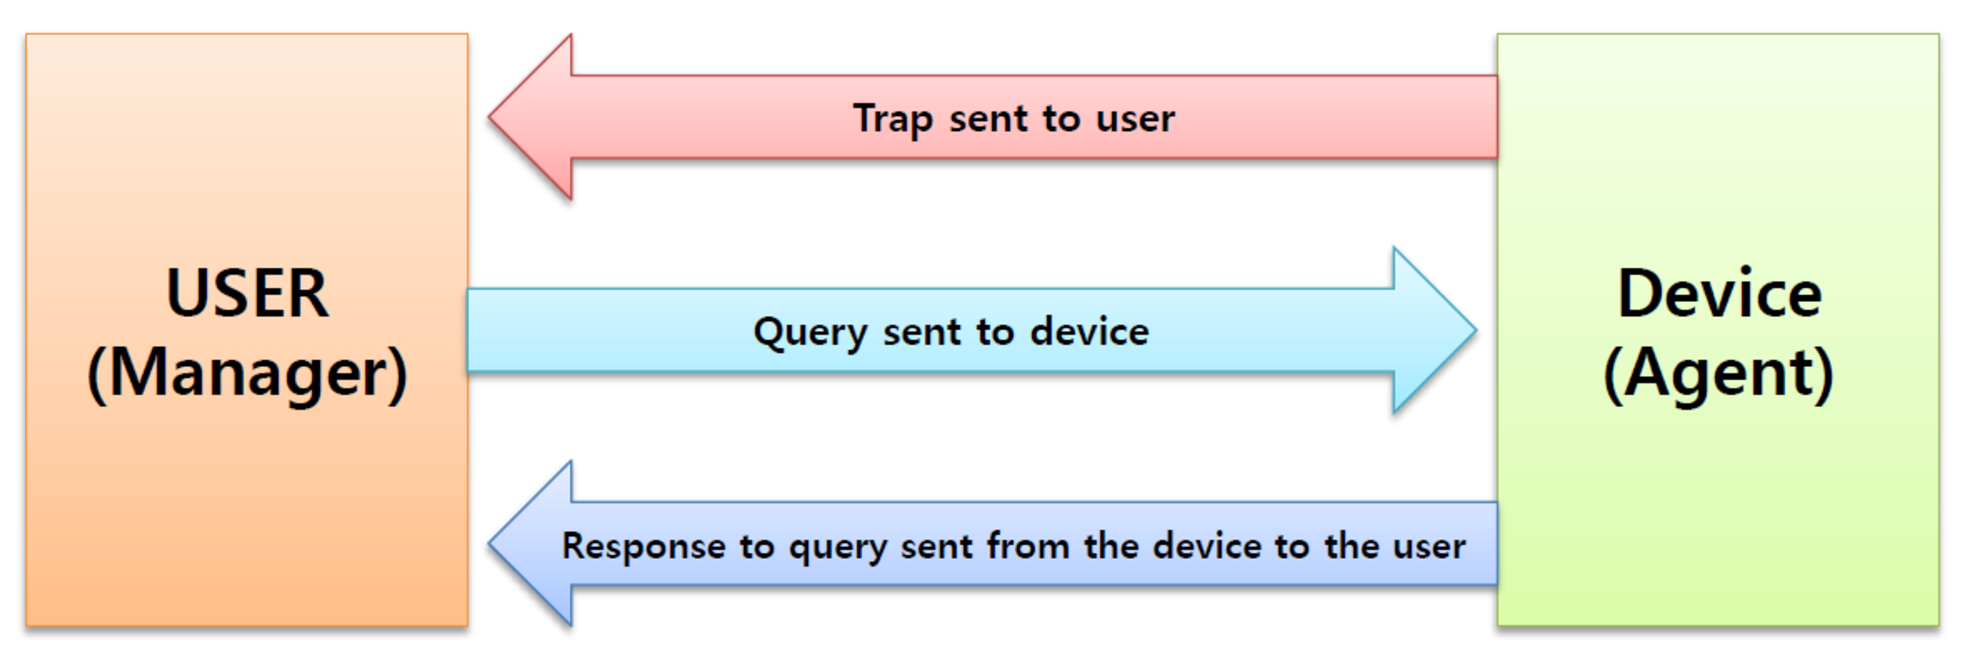
\includegraphics[width=0.65\textwidth]{./images/relationship_m_a.eps}
  \caption{Manager와 Agent의 관계}
  \label{fig:relationship_m_a}   
\end{figure}

\hfil\break
\hfil\break
\hfil\break
\hfil\break

SNMP는 v1/2c/3의 세 가지 버전이 있으며, 각 버전들은 인증과 암호화에 따른 차이점이 있다. SNMPv1/2c는 Community string에 의존한 문자열 일치로 사용자 인증을 하지만 암호화 하지 않는다. 반면 v3는 username을 통힌 사용자 인증 및 암호화 알고리즘(MD5, SHA, DES, AES)을 통한 인증과 암호화에 따라 noAuthNoPriv, authNoPriv, authPriv의 세 종류의 보안 레벨로 나뉜다. v3는 v1/2c에 비해 보안이 강화되지만 응답시간이 큰 단점이 있다. 자세한 SNMP 버전 별 차이점은 표 \ref{table:conparision}\citep{comparison}을 참조바란다.

\begin{table}[h!]
\begin{center}
\begin{tabular}{c|c|c|c}\hline
Version & Level & Authentication & Encryption \\ \hline
v1 & noAuthNoPriv & Community string & No \\ \hline
v2c & noAuthNoPriv & Community string & No \\ \hline
 & noAuthNoPriv & Username & No \\ \cline{2-4}
v3 & authNoPriv & MD5 or SHA & No \\ \cline{2-4}
 & authPriv & MD5 or SHA & DES or AES \\ \hline
\end{tabular}
\caption{SNMP 버전 별 차이점}
  \label{table:conparision} 
\end{center}
\end{table} 

\clearpage
\section{MIB(Management Information Base)}
SNMP를 지원하는 장치들은 MIB를 가지고 있으며, MIB는 관리되어야 할 장비에 대한 객체들을 계층구조로 모아 놓은 것으로 관리의 편의를 위해 그림 \ref{fig:oid_tree}와 같이 ROOT-Node에서 시작해 branch node와 leaf node로 이뤄진 Tree 구조를 가진다. 일반적인 TCP/IP관리정보는 MIB-2(RFC 1213)에 포함돼 있고, 특정 장비 관련 정보는 장비제조업체에서 제공한다. 

\begin{figure}[h!]
  \centering
  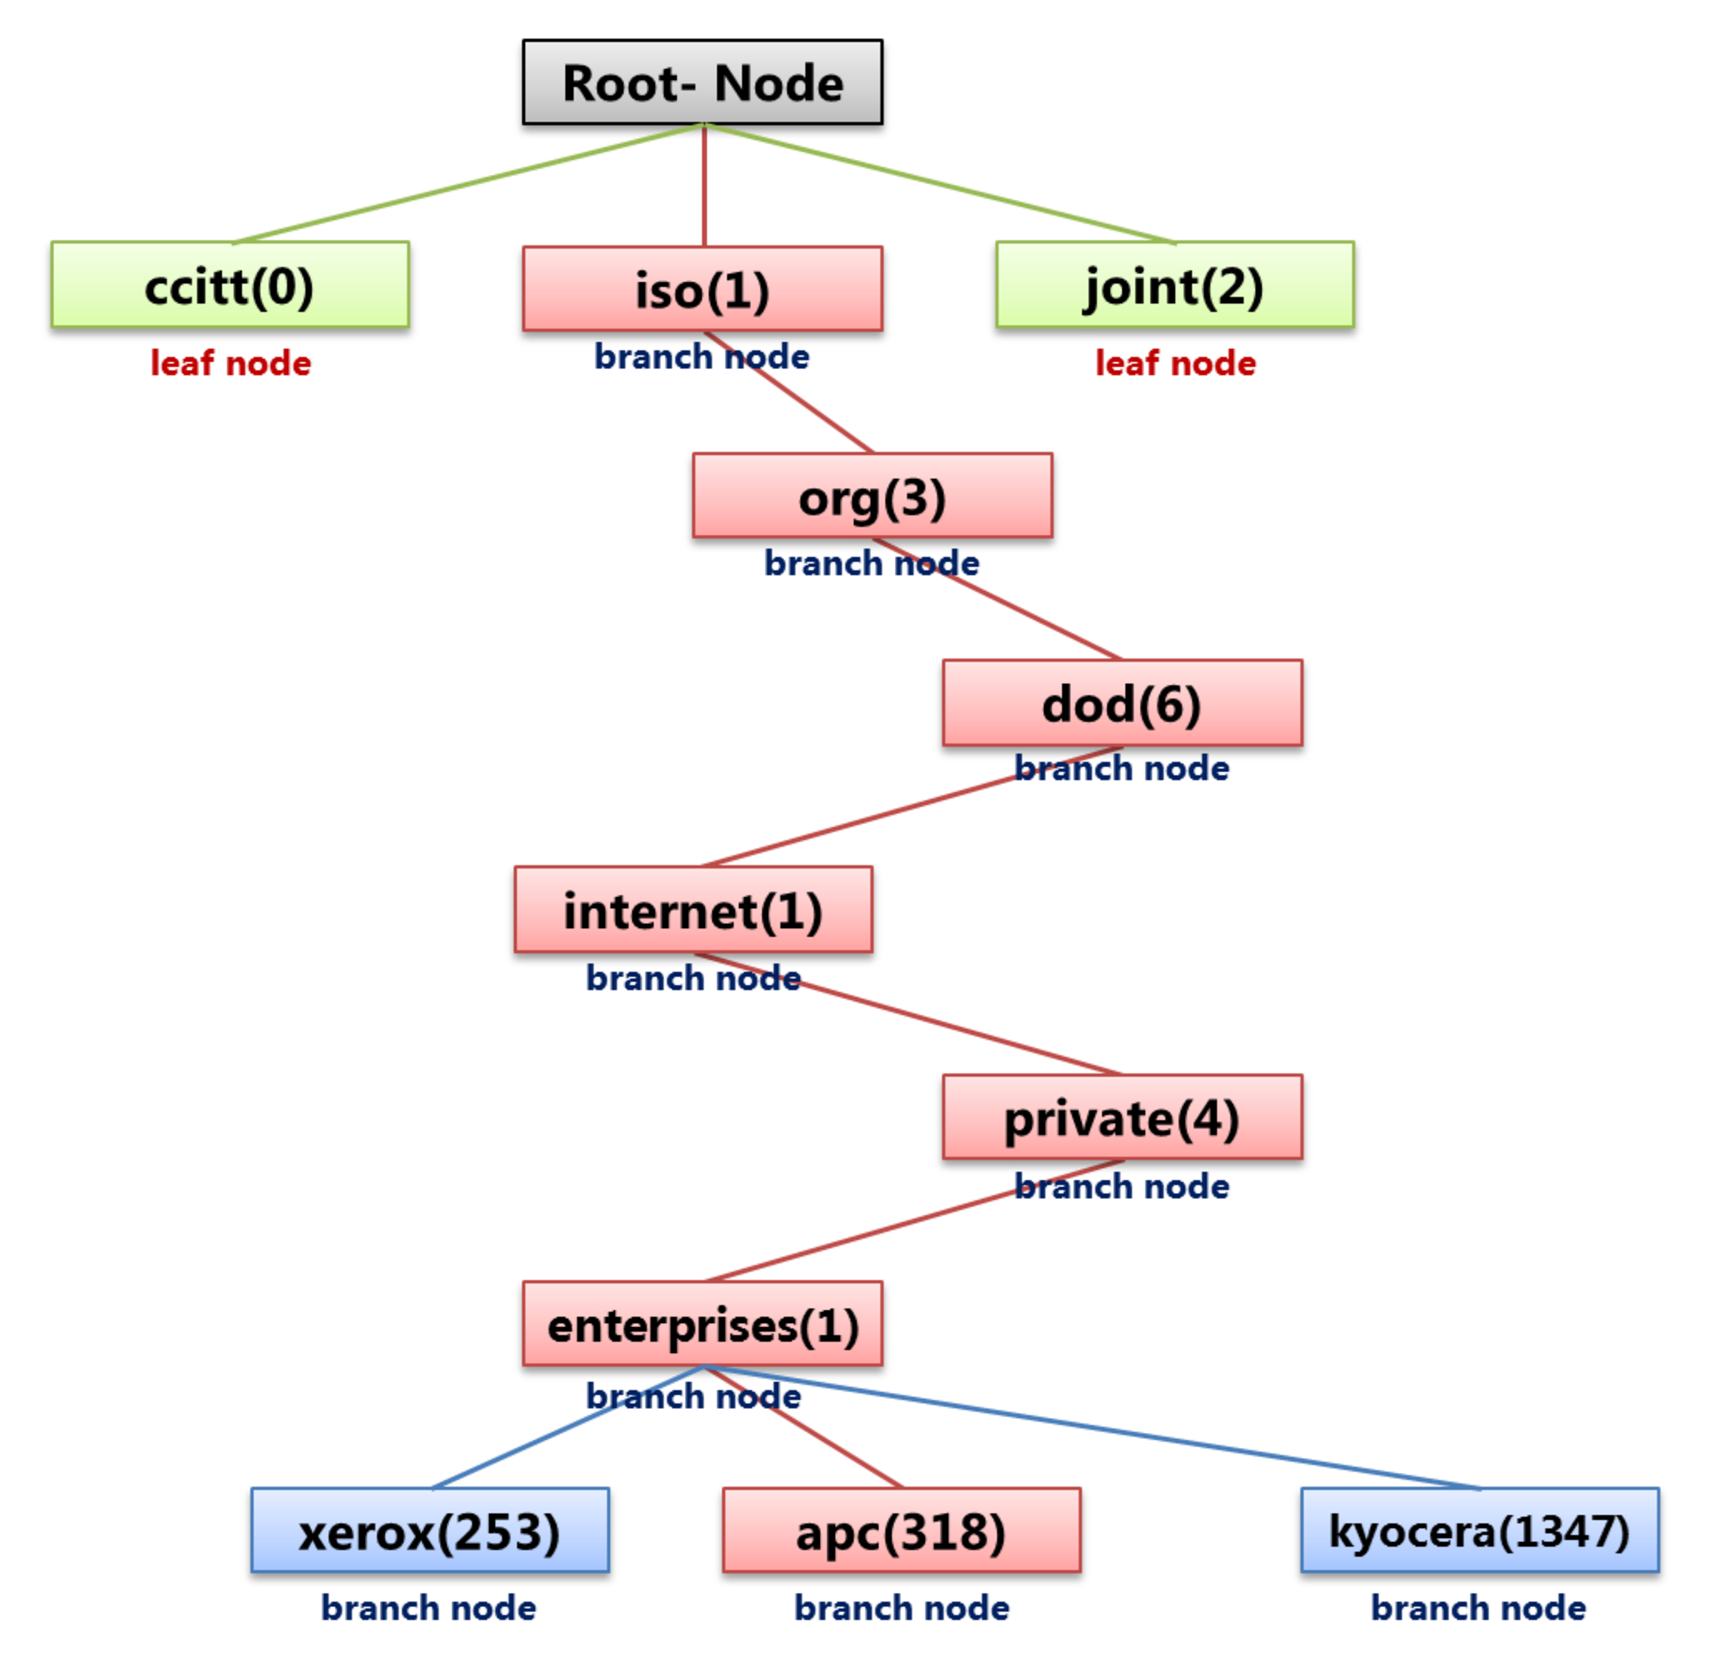
\includegraphics[width=0.65\textwidth]{./images/oidtree.eps}
  \caption{MIB의 일반적 구조}
  \label{fig:oid_tree} 
\end{figure}

MIB내의 객체들은 고유의 식별자를 가지며 이를 OID(Object Identifiers)라 한다. 그림 \ref{fig:oid_tree}를 참고하면 APC사의 OID는 세 종류의 표기법에 따라 아래와 같이 표현된다.
\begin{itemize}
\item OID 번호 \par  1.3.6.1.4.1.318
\item 객체 이름 \par iso.org.dod.internet.private.enterprises.apc 
\item 혼용 \par iso(1).org(3).dod(6).internet(1).private(4).enterprises(1).apc(318)
\end{itemize}

OID는 그림 \ref{fig:ex_mib}과 같은 포맷을 가지며 이를 통해 객체의 데이터 타입, 필요 유무, 정의 그리고 접근권한(read-only, read-write, etc...)에 대해 알 수 있다. 

\begin{figure}[h!]
  \centering
  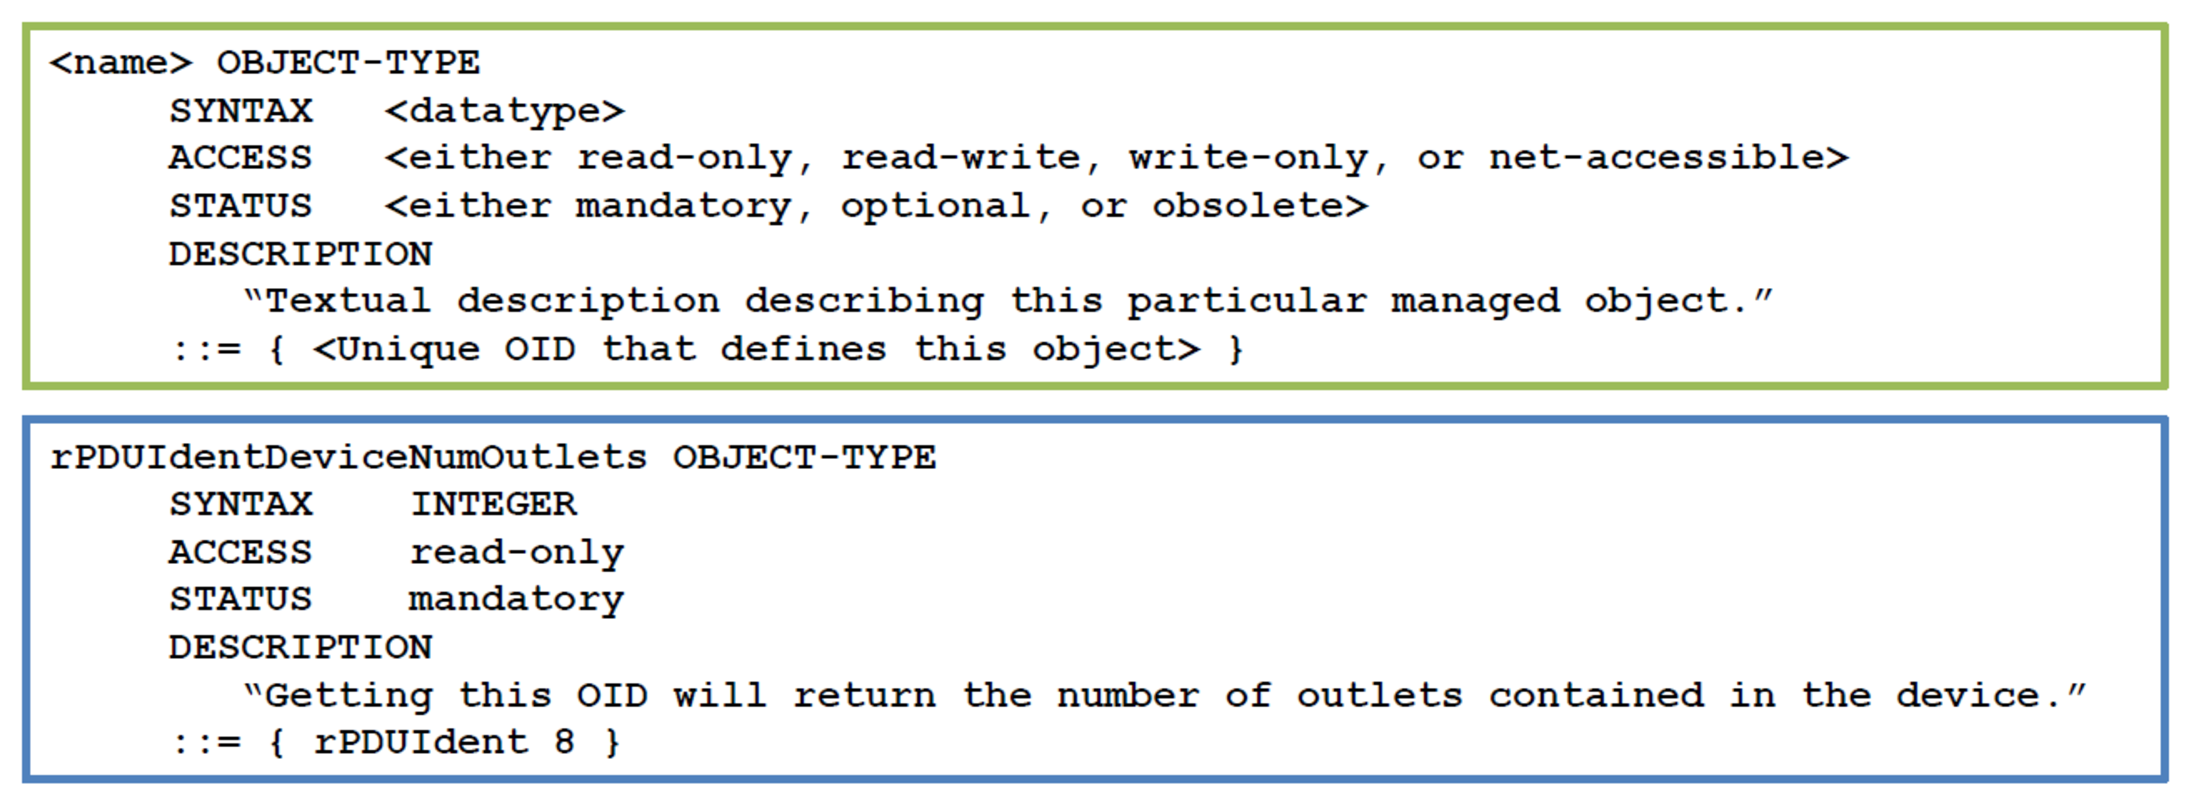
\includegraphics[width=0.8\textwidth]{./images/ex_mib.eps}
  \caption{OID 포맷의 예}
  \label{fig:ex_mib}   
\end{figure}


\subsection{1.2.1 MIB 파일 설정}
사용하고자 하는 장비의 MIB파일을 .snmp/snmp.conf파일(그림 \ref{fig:snmp_conf})에 추가하면 복잡한 OID번호 대신 MIB파일 내 객체 이름을 사용하여 장비의 정보를 요청할 수 있다.
snmp.conf 파일에 추가하기 앞서 MIB파일의 DEFINITIONS에 정의된 이름과 파일의 이름이 다를 경우 약간의 수정이 필요하다. 
\begin{figure}[h]
  \centering
  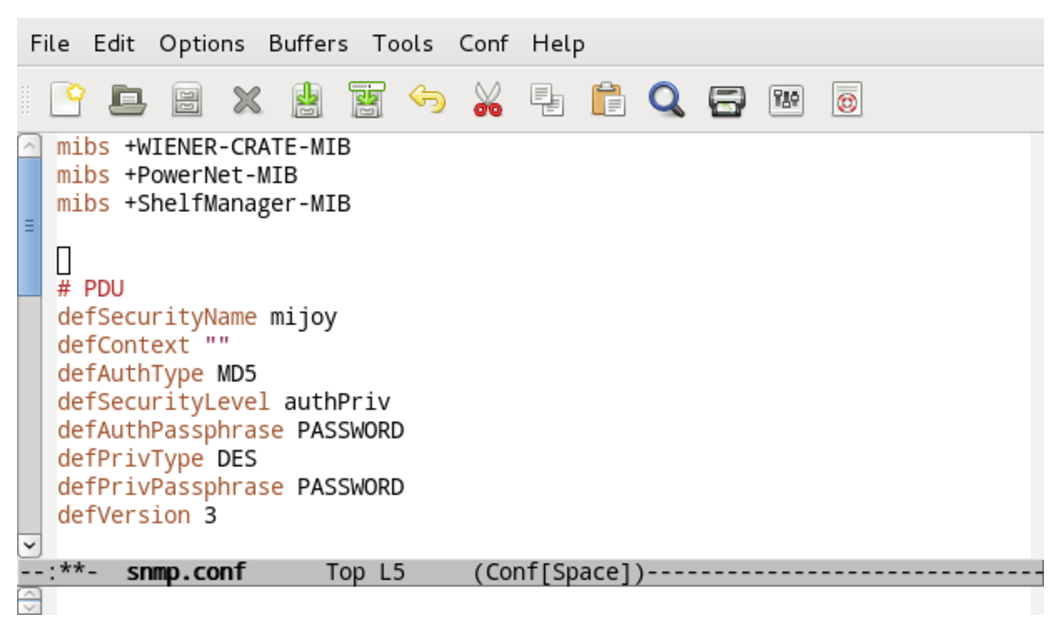
\includegraphics[width=0.79\textwidth]{./images/snmp_conf.eps}
  \caption{snmp.conf 파일}
  \label{fig:snmp_conf}   
\end{figure}

그림 \ref{fig:pdu_mib}는 APC사 PDU의 MIB파일의 일부분으로 다음과 같이 MIB파일의 DEFINITIONS ::= BEGIN에 파일의 이름(PowerNet-MIB)을 정의해주고, MIB파일명도 동일하게(PowerNet-MIB) 저장하면 된다. 이 과정을 거치면 OID번호가 아닌 객체 이름으로 장비의 정보를 읽고 쓸 수 있다. 


\begin{figure}[h]
  \centering
  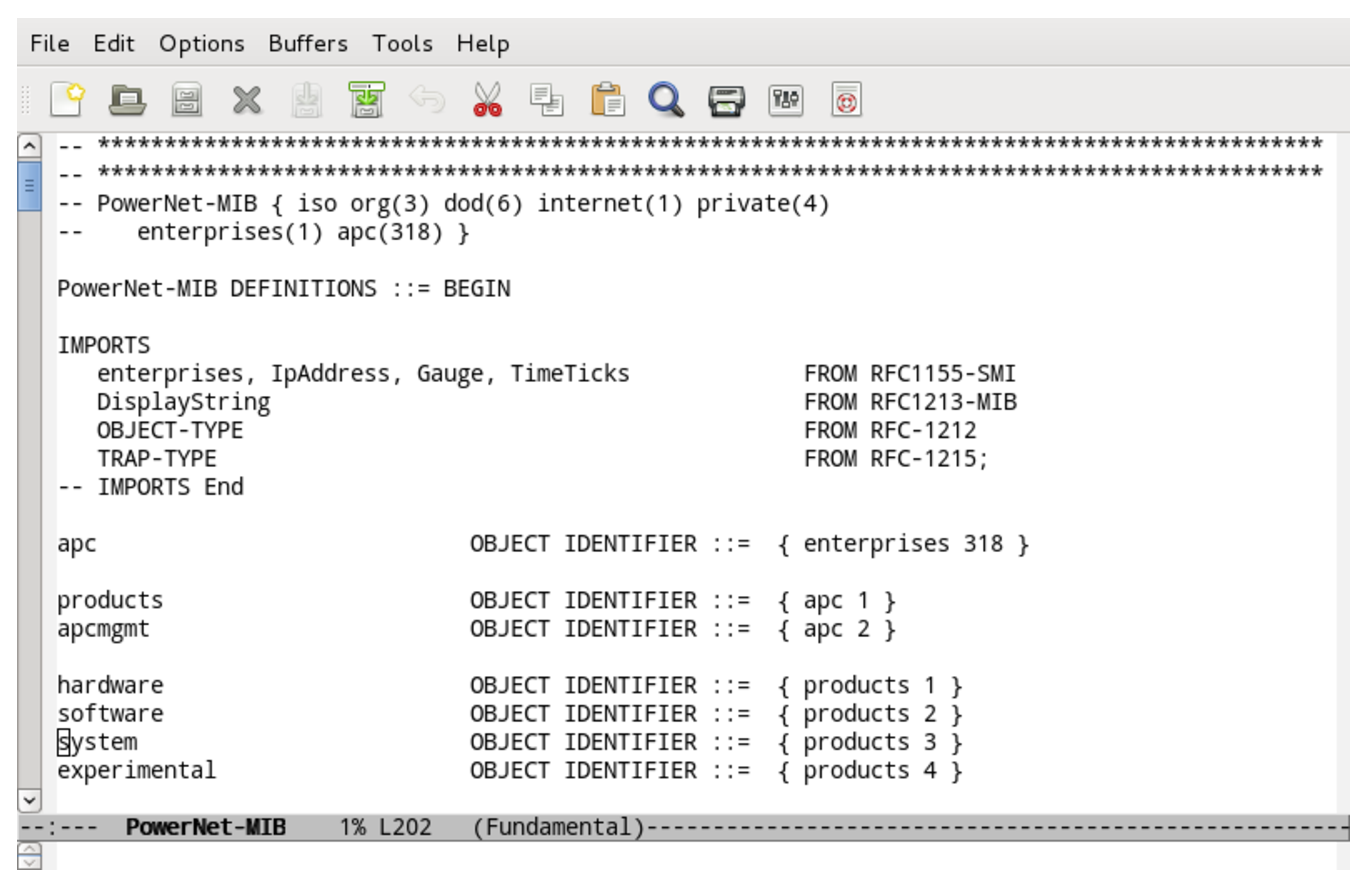
\includegraphics[width=0.79\textwidth]{./images/pdu_mib.eps}
  \caption{APC사 PDU의 MIB파일}
  \label{fig:pdu_mib}   
\end{figure}


\clearpage

\chapter{SNMP의 설치 및 사용}
\section{설치}
SNMP를 사용에 앞서 아래의 패키지를 설치해야 한다. 본 문서에서는 NET-SNMP\citep{net_snmp} v5.4.3을 사용하고 있다.
\begin{itemize}
\item NET-SNMP\footnote{* NET-SNMP는 http://www.net-snmp.org/download.html에서 다운받을 수 있다.}
\item snmp snmpd
\item snmp-mibs-downloader
\item libsnmp-dev libsnmp-base libsnmp-perl libsnmp15 
\end{itemize}


\section{SNMP 명령어와 사용}

\subsection{2.2.1 SNMPv3 설정}
SNMPv1/2c와 달리 SNMPv3는 보안레벨에 따른 인증과 암호화의 이유로 username, 알고리즘 그리고 패스워드 설정이 필요하다. 각 장비의 v3 관련 설정은 그림 \ref{fig:apc_v3}과 같이 장비제조업체에서 제공하는 웹 페이지, 프로그램, 시리얼 통신을 통해 설정할 수 있다. localhost의 SNMPv3 설정은 다음과 같이 net-snmp의 snmpd로 가능하다. 이때, 패스워드는 적어도 8자 이상이어야 한다.


\begin{figure}[h]
  \centering
  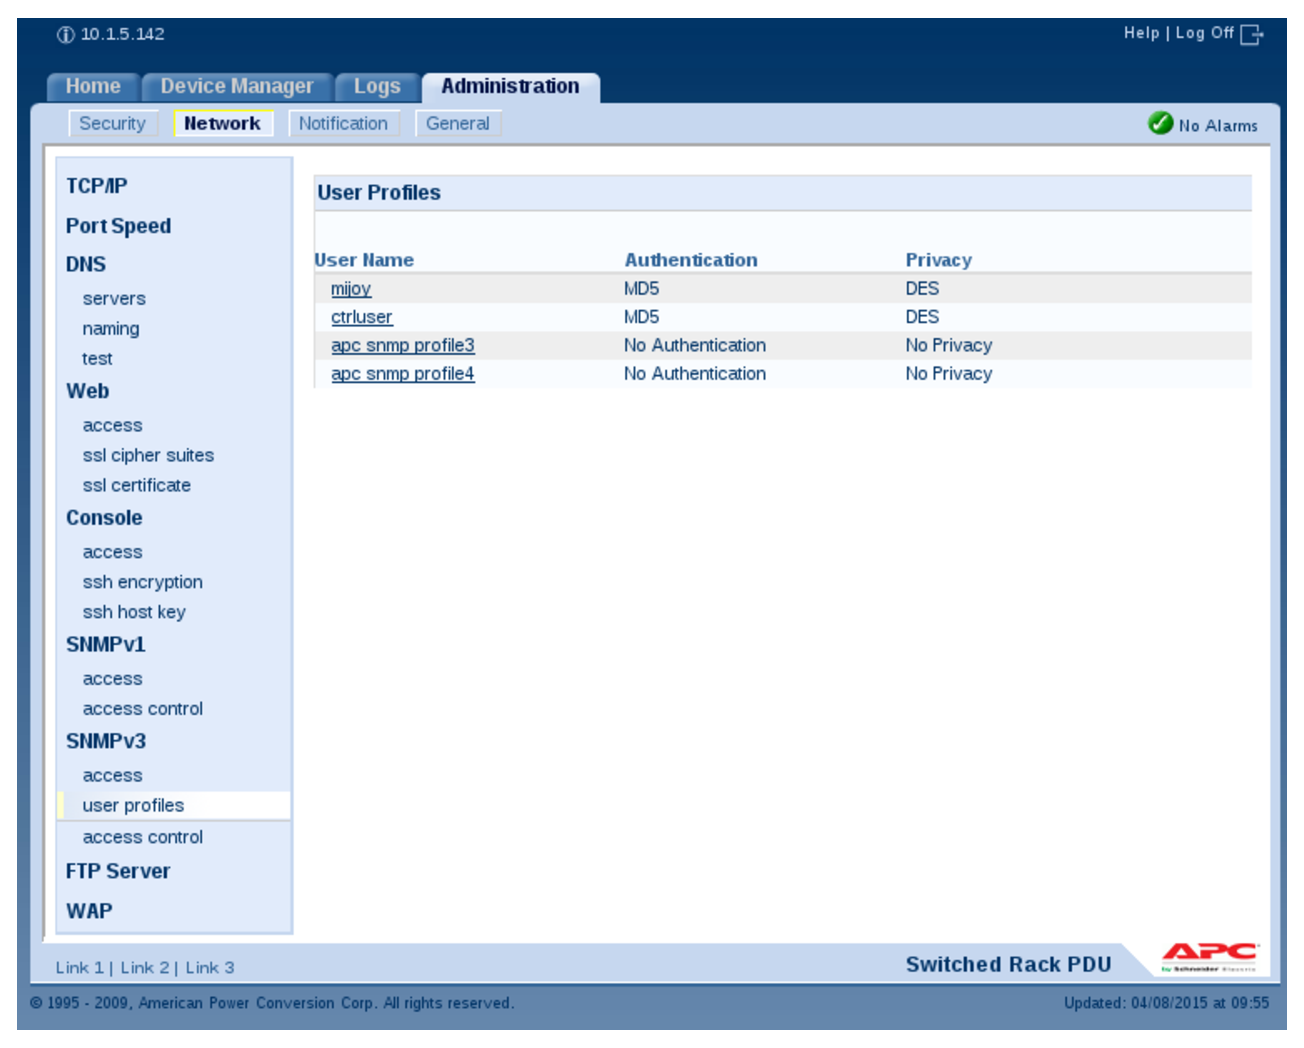
\includegraphics[width=0.79\textwidth]{./images/apcv3.eps}
  \caption{APC사의 장비설정 웹 페이지}
  \label{fig:apc_v3}   
\end{figure}




\begin{lstlisting}[style=termstyle]
mijoy0909@mjpark:~$ su                                     
root@mjpark:~# service snmpd stop
Stopping network management services: snmpd snmptrapd.
root@mjpark:~# net-snmp-config --create-snmpv3-user
Enter a SNMPv3 user name to create: 
mijoy
Enter authentication pass-phrase: 
[password]
Enter encryption pass-phrase: 
  [press return to reuse the authentication pass-phrase]
[password]
adding the following line to /var/lib/snmp/snmpd.conf:
   createUser test MD5 "[password]" DES [password]
adding the following line to /usr/share/snmp/snmpd.conf:
   rwuser mijoy 
root@mjpark:~# service snmpd start
Starting network management services: snmpd.
\end{lstlisting}

snmpd의 설정은 /usr/share/snmp/snmpd.conf에서 아래와 같이 확인 가능하다. \footnote{* http://www.net-snmp.org/docs/README.snmpv3.html 참조 바람}

\begin{lstlisting}[style=termstyle]
rwuser mijoy
\end{lstlisting}


\subsection{2.2.2 SNMP 명령어}
SNMP를 이용해 장비의 정보를 요청하기 위해서는 SNMP명령어\footnote{* 자세한 설명은 http://www.net-snmp.org/wiki/index.php/Tutorials를 참조 바람}가 사용되며, 명령어는 SNMP의 버전에 따라 차이가 있다.

\begin{itemize}
\item get : Manager가 Agent에게 특정 정보를 요청 시 사용
\item getnext : get과 동일, 동일 계층의 다음 정보를 요청 시 사용
\item walk : get의 확장 형태, Tree구조에서 하위 트리들의 정보를 요청 시 사용
\item set : Manager가 특정 값을 변경 및 설정 시 사용
\item trap : Agent가 비동기적 사건을 Manager에게 알리기 위해 사용
\item etc...
\end{itemize}

\clearpage

자주 사용되는 SNMP 옵션은 다음와 같다. 이 외의 추가적인 옵션은 snmp(walk, get, set, trap...) -h를 이용해 알 수 있다.

\begin{itemize}
\item -v 1/2c/3 : SNMP 버전
\item -c : v1/2c 사용자 (Community string)
\item -u : v3 사용자 (Username)
\item -a MD5/SHA : v3 authentication 암호화 알고리즘
\item -A : authentication 패스워드
\item -x DES/AES : v3 privacy 암호화 알고리즘
\item -X : privacy 패스워드
\item -m : 사용할 MIB파일
\item etc...
\end{itemize}


\subsection{2.2.3 SNMP 명령어 사용 1 (walk, get)}
\subsubsection{- SNMPv1/2c}

\begin{lstlisting}[style=termstyle]
snmp(walk, get) -v (v1/2c) -c (Community String) (HostAddress) (OID) 
\end{lstlisting}

v1/2c에서 사용자 인증에 사용하는 Community string은 대부분 public/privacy/admin 중 하나로 설정되어 장비제조업체에서 제공되지만, 사용자가 임의로 변경할 수 있다. public은 read-only 권한을 privacy, admin은 read-write의 권한을 가지고 있다. 따라서 public을 이용하여 장비의 정보 값을 변경할 수 없다. v1/2c는 Community string을 사용한 사용자 인증 외에는 특별한 보안이 없어 보안에 취약하다는 것을 알 수 있다. 
\begin{lstlisting}[style=termstyle]
mijoy0909@mjpark:~$ snmpwalk -v 1 -c public localhost
RFC1213-MIB::sysDescr.0 = STRING: "Linux mjpark 3.2.0-4-amd64 #1 SMP Debian 3.2.63-2+deb7u2 x86_64"
RFC1213-MIB::sysObjectID.0 = OID: SNMPv2-SMI::enterprises.8072.3.2.10
RFC1213-MIB::sysUpTime.0 = Timeticks: (49138) 0:08:11.38
RFC1213-MIB::sysContact.0 = STRING: "Me <me@example.org>"
RFC1213-MIB::sysName.0 = STRING: "mjpark"
.
.
.
real	0m1.440s
user	0m0.224s
sys	0m0.084s
--------------------------------------------------------------------------------------------------
mijoy0909@mjpark:~$ snmpwalk -v 2c -c public localhost
RFC1213-MIB::sysDescr.0 = STRING: "Linux mjpark 3.2.0-4-amd64 #1 SMP Debian 3.2.63-2+deb7u2 x86_64"
RFC1213-MIB::sysObjectID.0 = OID: SNMPv2-SMI::enterprises.8072.3.2.10
RFC1213-MIB::sysUpTime.0 = Timeticks: (49138) 0:08:11.38
RFC1213-MIB::sysContact.0 = STRING: "Me <me@example.org>"
RFC1213-MIB::sysName.0 = STRING: "mjpark"
.
.
.
real	0m1.422s
user	0m0.220s
sys	0m0.096s
\end{lstlisting}

위의 결과는 아래의 결과는 snmpwalk명령어로 요청한 localhost의 정보 일부와 linux time command를 이용해 요청의 응답에 걸린 시간을 측정한 결과이다. v1/2c는 버전의 차이 외에 사용의 차이가 없지만, Community string을 사용한 사용자 인증 외에 추가적인 보안이 없어 보안에 취약하다는 것을 알 수 있다.


장비의 모든 정보만 요청하는 snmpwalk와 달리 snmpget을 이용하면 아래와 같이 필요한 정보의 값을 선택적으로 읽을 수 있다.
\begin{lstlisting}[style=termstyle]
mijoy0909@mjpark:~$ snmpget -v 2c -c public localhost RFC1213-MIB::sysName.0
RFC1213-MIB::sysName.0 = STRING: "mjpark"
.
.

mijoy0909@mjpark:~$ snmpget -v 1 -c public localhost RFC1213-MIB::sysName.0 RFC1213-MIB::sysObjectID.0
RFC1213-MIB::sysName.0 = STRING: "mjpark"
RFC1213-MIB::sysObjectID.0 = OID: SNMPv2-SMI::enterprises.8072.3.2.10
\end{lstlisting}


\subsubsection{- SNMPv3}
v3는 v1/2c와 달리 Username을 사용하므로 –u옵션을 사용하고 암호화 알고리즘에 대한 옵션들이 추가되며, 기본 포맷은 다음과 같다.
\begin{lstlisting}[style=termstyle]
snmp(walk, get) -v 3 -u (Username) -l {Security Level(noAuthNoPriv/authNoPriv/authPrive)} -a {Authentication Protocol(MD5/SHA)} -A (PASSWORD) -x {Privacy Protocol(DES/AES)} -X (PASSWORD) (HostAddress) (OID) 
\end{lstlisting}

snmpwalk를 이용해 요청한 localhost의 정보 일부와 응답시간은 다음과 같다. v1/2c와 요청에 대한 응답의 차이는 없지만, 응답시간이 더 소요됨을 알 수 있다.

\begin{lstlisting}[style=termstyle]
mijoy0909@mjpark:~$ snmpwalk -v 3 -u mijoy -l authPriv -a MD5 -A  [PASSWORD]  -x DES -X  [PASSWORD]  localhost
RFC1213-MIB::sysDescr.0 = STRING: "Linux mjpark 3.2.0-4-amd64 #1 SMP Debian 3.2.63-2+deb7u2 x86_64"
RFC1213-MIB::sysObjectID.0 = OID: SNMPv2-SMI::enterprises.8072.3.2.10
RFC1213-MIB::sysUpTime.0 = Timeticks: (32928) 0:05:29.28
RFC1213-MIB::sysContact.0 = STRING: "Me <me@example.org>"
RFC1213-MIB::sysName.0 = STRING: "mjpark"
.
.
.
real	0m1.773s
user	0m0.340s
sys	0m0.124s
\end{lstlisting}


\subsection{2.2.4 SNMP 명령어 사용 2 (set)}

snmpwalk, get과 달리 set은 장비의 정보를 설정 및 변경하고자 할 때 사용된다. 이 때, 아래와 같이 객체가 가진 데이터 타입에 따른 옵션이 필요하다.

\begin{lstlisting}[style=termstyle]
 i: INTEGER 
 u: unsigned INTEGER 
 t: TIMETICKS
 a: IPADDRESS
 o: OBJID
 s: STRING
 x: HEX STRING
 d: DECIMAL STRING
 U: unsigned int64
 I: signed int64
 F: float
 D: double
\end{lstlisting}

버전별 snmpset명령어는 snmpwalk, get의 포맷에 데이터 타입과 값의 정보가 추가된 기본 포맷을 가진다.

\subsubsection{- SNMPv1/2c}

\begin{lstlisting}[style=termstyle]
mijoy0909@mjpark:~$ snmpset -v (v1/2c) -c (Community String) (HostAddress) (OID) (datatypes) (value)
\end{lstlisting}

\subsubsection{- SNMPv3}

\begin{lstlisting}[style=termstyle]
mijoy0909@mjpark:~$ snmpset -v 3 -u (Username) -l {Security Level(noAuthNoPriv/authNoPriv/authPrive)} -a {Authentication Protocol(MD5/SHA)} -A (PASSWORD) -x {Privacy Protocol(DES/AES)} -X (PASSWORD) (HostAddress) (OID) (datatypes) (value)
\end{lstlisting}

다음은 APC사의 Power Distribution Unit의 Outlet8번의 전원을 v3를 이용하여 설정한 결과이다. 

\begin{lstlisting}[style=termstyle]
mijoy0909@mjpark:~$ snmpset -v 3 -u mijoy -l authPriv -a MD5 -A [PASSWORD] -x DES -X [PASSWORD] 10.1.5.142 sPDUOutletCtl.8 i 2
PowerNet-MIB::sPDUOutletCtl.8 = INTEGER: outletOff(2)
.
.
mijoy0909@mjpark:~$ snmpset -v 3 -u mijoy -l authPriv -a MD5 -A [PASSWORD] -x DES -X [PASSWORD] 10.1.5.142 sPDUOutletCtl.7 i 1 sPDUOutletCtl.8 i 1
PowerNet-MIB::sPDUOutletCtl.7 = INTEGER: outletOn(1)
PowerNet-MIB::sPDUOutletCtl.8 = INTEGER: outletOn(1)
\end{lstlisting}

v1/2c에 비해 긴 v3의 명령어는 반복 사용에 어려움이 있다. 따라서 그림 \ref{fig:snmp_conf}와 같이 snmp.conf 파일에 장비의 v3에 대한 보안레벨, 암호화 알고리즘, 패스워드에 대한 정보를 미리 저장해둔다면 아래와 같이 간단한 명령어로 v3를 사용할 수 있다.\footnote{* 여러가지 장비의 정보를 설정한 후 장비의 정보를 요청한 결과 첫 번째로 저장된 설정에서만 간편하게 SNMPv3 사용이 가능하였다. 이는 추가적인 확인이 필요한데, 만약 첫 번째로 저장된 설정에서만 가능하다면 v3를 사용하고자 하는 장비의 보안레벨, 암호화 프로토콜, 그리고 패스워드를 통일하는 작업이 필요 할 것 같다.}

\begin{lstlisting}[style=termstyle]
mijoy0909@mjpark:~$ snmpget 10.1.5.142 sPDUIdentModelNumber
PowerNet-MIB::sPDUIdentModelNumber.0 = STRING: "AP7921"
\end{lstlisting}


\clearpage
\section{SNMP를 이용한 장비 모니터링}
본 문서에 사용된 시스템, 소프트웨어 및 하드웨어의 정보 그리고 장비제조업체에서 지원하는 SNMP버전\footnote{*본 문서에서 Read는 모니터링, Write는 제어라 칭한다.}은 다음과 같다.
\subsection{2.3.1 시스템 및 소프트웨어}
\begin{itemize}
\item Debian Linux 7 Wheezy
\item NET-SNMP v5.4.3
\item GNU Bash script-CLI(Command-line Interface) 
\end{itemize}

\subsection{2.3.2 하드웨어 및 SNMP지원버전\ref{table:used_version}}

\begin{table}[h]
\begin{center}
\begin{tabular}{c|c}\hline
Device Name & Supported Versions \\ \hline
Printer(Xerox, Kyocera) & v1* (R) \\ \hline
WIENER VME CRATE & v1/2c* (R/W) \\ \hline
ELMA VME CRATE & v3* (R) \\ \hline
APC PDU 7921 & v1/2c/3* (R/W) \\ \hline
\end{tabular}
\caption{모니터링에 사용된 장비와 장비 별 지원하는 SNMP 버전}
{(R: Read, W: Write / *: 모니터링에 사용된 버전)}
  \label{table:used_version}  
\end{center}
\end{table} 

\clearpage
\subsection{2.3.3 모니터링 결과}
\subsubsection{2.3.3.1 프린터(Xerox \& Kyocera)}

가속기 제어에 사용되는 장비에 앞서 Xerox사와 Kyocera사의 네트워크 프린터들에 기본 설정된 사항으로 프린터 용지의 종류와 양, 잉크의 잔여량 등의 상태 정보를 SNMPv1로 모니터링한 결과이다. 모니터링 결과에서 182 Printer는 Xerox사, 184 Printer는 Kyocera사의 프린터이다.

\begin{lstlisting}[style=termstyle, caption=Xerox \& Kyocera사 Printer 모니터링 결과]]
mijoy0909@mjpark:~/users/mijoy0909$ ./snmptest.sh 
 
Mon Nov 17 10:35:17 KST 2014
 
++++++++++++++++ Printer Status ++++++++++++++++
- 182 Printer              -, "Printing..." "" ""
- 184 Printer              -, "Sleeping " " "
 
++++++++ 182 Printer Paper Current Level ++++++++
- Tray1                    -, 25.000%
- Tray2                    -, 0%
- Tray3                    -, 75.000%
- Tray4                    -, 75.000%
- Tray5                    -, 0%
 
++++++++ 182 Printer Paper Current size ++++++++
- Tray1                    -, A4
- Tray2                    -, A4
- Tray3                    -, A4
- Tray4                    -, A3
- Tray5                    -, -
 
++++++++ 184 Printer Paper Current Level ++++++++
- MP Tray                  -, 0%
- Tray1                    -, 50.000%
- Tray2                    -, 0%
- Tray3                    -, 50.000%
- Tray4                    -, 50.000%
 
++++++++ 184 Printer Paper Current size ++++++++
- MP Tray                  -, A4
- Tray1                    -, A4
- Tray2                    -, -
- Tray3                    -, A3
- Tray4                    -, A3
 
++++++++ 182 Printer Toner Current Level ++++++++
- black                    -, 97.000%
- yellow                   -, 6.000%
- magenta                  -, 9.000%
- cyan                     -, 40.000%
 
++++++++ 184 Printer Toner Current Level ++++++++
- black                    -, 73.000%
 
+++++++++ 182 Printer Printed Page(s) ++++++++++
- total                    -, 477124
 
+++++++++ 184 Printer Printed Page(s) ++++++++++
- total                    -, 86618
\end{lstlisting}


\subsubsection{2.3.3.2 VMEbus Crate(Elma \& Wiener)}
VMEbus Crate(그림 \ref{fig:elmawiener})는 가속기를 제어하는 데 있어 중요한 장비들이며, 가속기 시설의 특성상 즉각적인 접근이 불가능한 지역에 설치되는 경우가 많다. 이러한 이유로 다른 장비들과 다르게 모니터링 및 제어를 할 수 있어야 하며, 신호의 보안에도 신경을 써야 한다.

\begin{figure}[h]
  \centering
  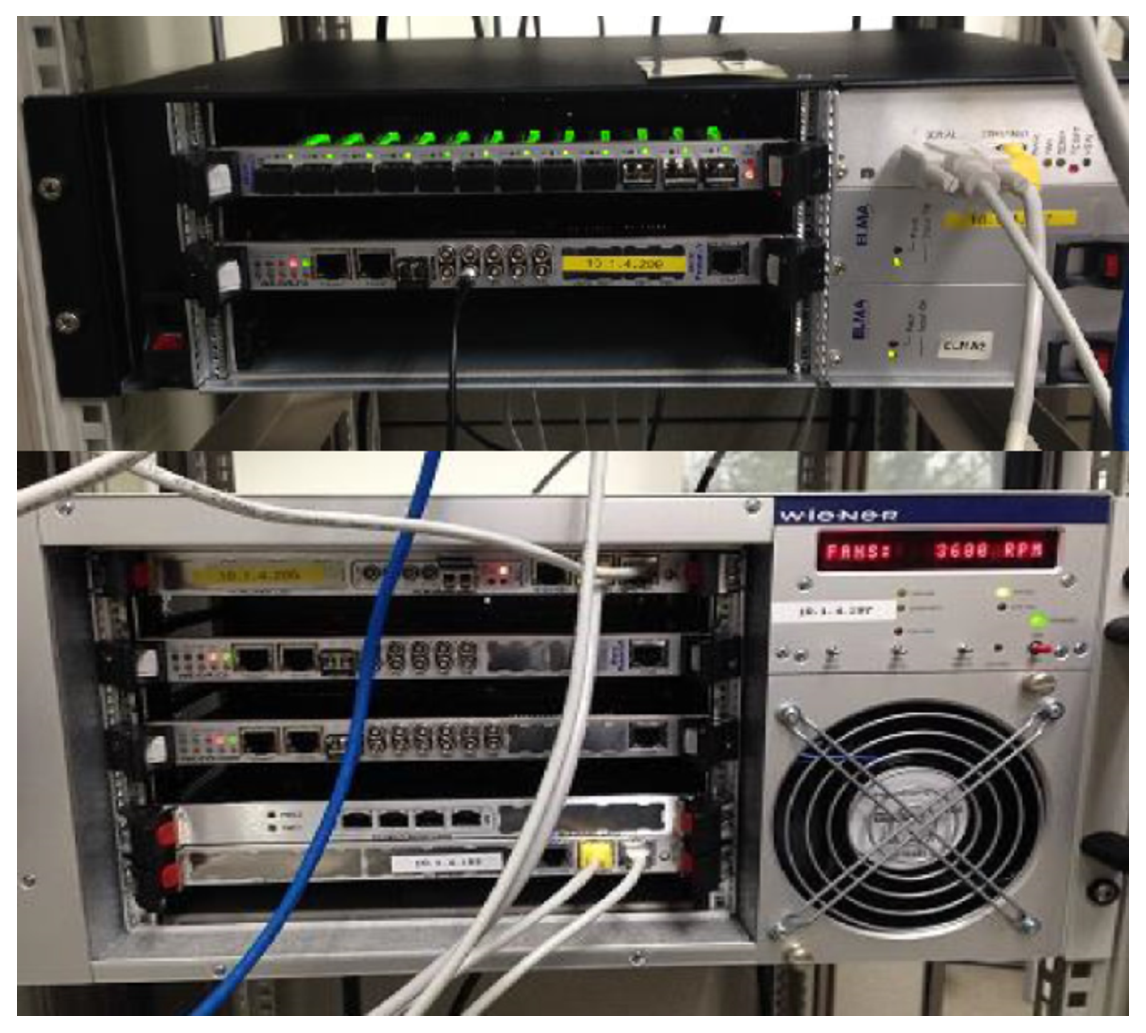
\includegraphics[width=0.7\textwidth]{./images/elmawiener.eps}
  \caption{Elma, Wiener Crate (위 : Elma, 아래: Wiener)}
  \label{fig:elmawiener}   
\end{figure}

\vspace{2mm}

본 문서에서 SNMPv3의 Read만 지원하는 Elma사의 Crate는 온도, 팬 스피드 등의 Crate 상태 모니터링 CLI를 구현하였고, SNMPv2c의 Read/Write를 모두 지원한 Wiener사의 Crate는 상태 모니터링뿐만 아니라 스위치의 전원과 팬 스피드를 제어할 수 있도록 구현되었다. 

\clearpage

- Elma Crate
\begin{lstlisting}[style=termstyle, caption=ELMA Crate 모니터링 결과]]
mijoy0909@mjpark:~/users/mijoy0909$ ./elma_test1.sh

- Voltage
==================================================
   #         Name          Value          State
==================================================
   1     "+3.3V"          3.290 V          OK
   2       "+5V"          4.980 V          OK
   3      "+12V"         11.960 V          OK
   4      "-12V"         12.090 V          OK
==================================================

- Temp
==================================================
   #         Name          Value          State
==================================================
   1       "Temp 1"       37 deg C         OK
   2       "Temp 2"       27 deg C         OK
   3       "Temp 3"       24 deg C         OK
==================================================

- Fan
==================================================
   #         Name          Value          State
==================================================
   1        "Fan 1"       3400 RPM         OK
   2        "Fan 2"       3400 RPM         OK
   3        "Fan 3"       3400 RPM         OK
   4        "Fan 4"       3400 RPM         OK
   5        "Fan 5"       3500 RPM         OK
   6        "Fan 6"       3400 RPM         OK
==================================================
\end{lstlisting}

\clearpage
- Wiener Crate
\begin{lstlisting}[style=termstyle, caption=Wiener Crate 모니터링 및 제어결과]]
***************************************
*               OPTIONS               *
***************************************
  [s] Status                           
  [1] Main Switch ON/OFF               
  [2] Change Fan Speed (1200~3600 RPM) 
  [q] Exit                             
  [0] Help                             
***************************************
-> Please enter your choice : 2

- Main Switch : ON
- Fan Speed : 3500 RPM
- Temperature Sensors1 : 25 deg C
- Temperature Sensors2 : 22 deg C

- Voltage
========================================
 Name        Value          State
========================================
  U0         3.33 V           On
  U1         5.01 V           On
  U2        12.06 V           On
  U3       -12.24 V           On
========================================

Enter Fan Speed (0~3600 RPM) : 
3600
INTEGER: 3600 RPM

- Main Switch : ON
- Fan Speed : 3600 RPM
- Temperature Sensors1 : 25 deg C
- Temperature Sensors2 : 22 deg C
\end{lstlisting}

\clearpage
\subsubsection{2.3.3.3 Power Distribution Unit}
VMEbus Crate와 마찬가지로 Power supply 또한 장비의 전원관리를 위해 모니터링과 제어를 할 수 있어야 한다. SNMPv3 Read/Write를 지원하는 APC사의 PDU (Power Distribution Unit) 7921(그림 \ref{fig:apc_pdu})을 이용하여 장비의 사용전력, 부하된 전류량 등의 상태를 모니터링 하고, 장비가 지원하는 다양한 옵션으로 Power Outlet을 제어할 수 있도록 하였다.
\begin{figure}[h]
  \centering
  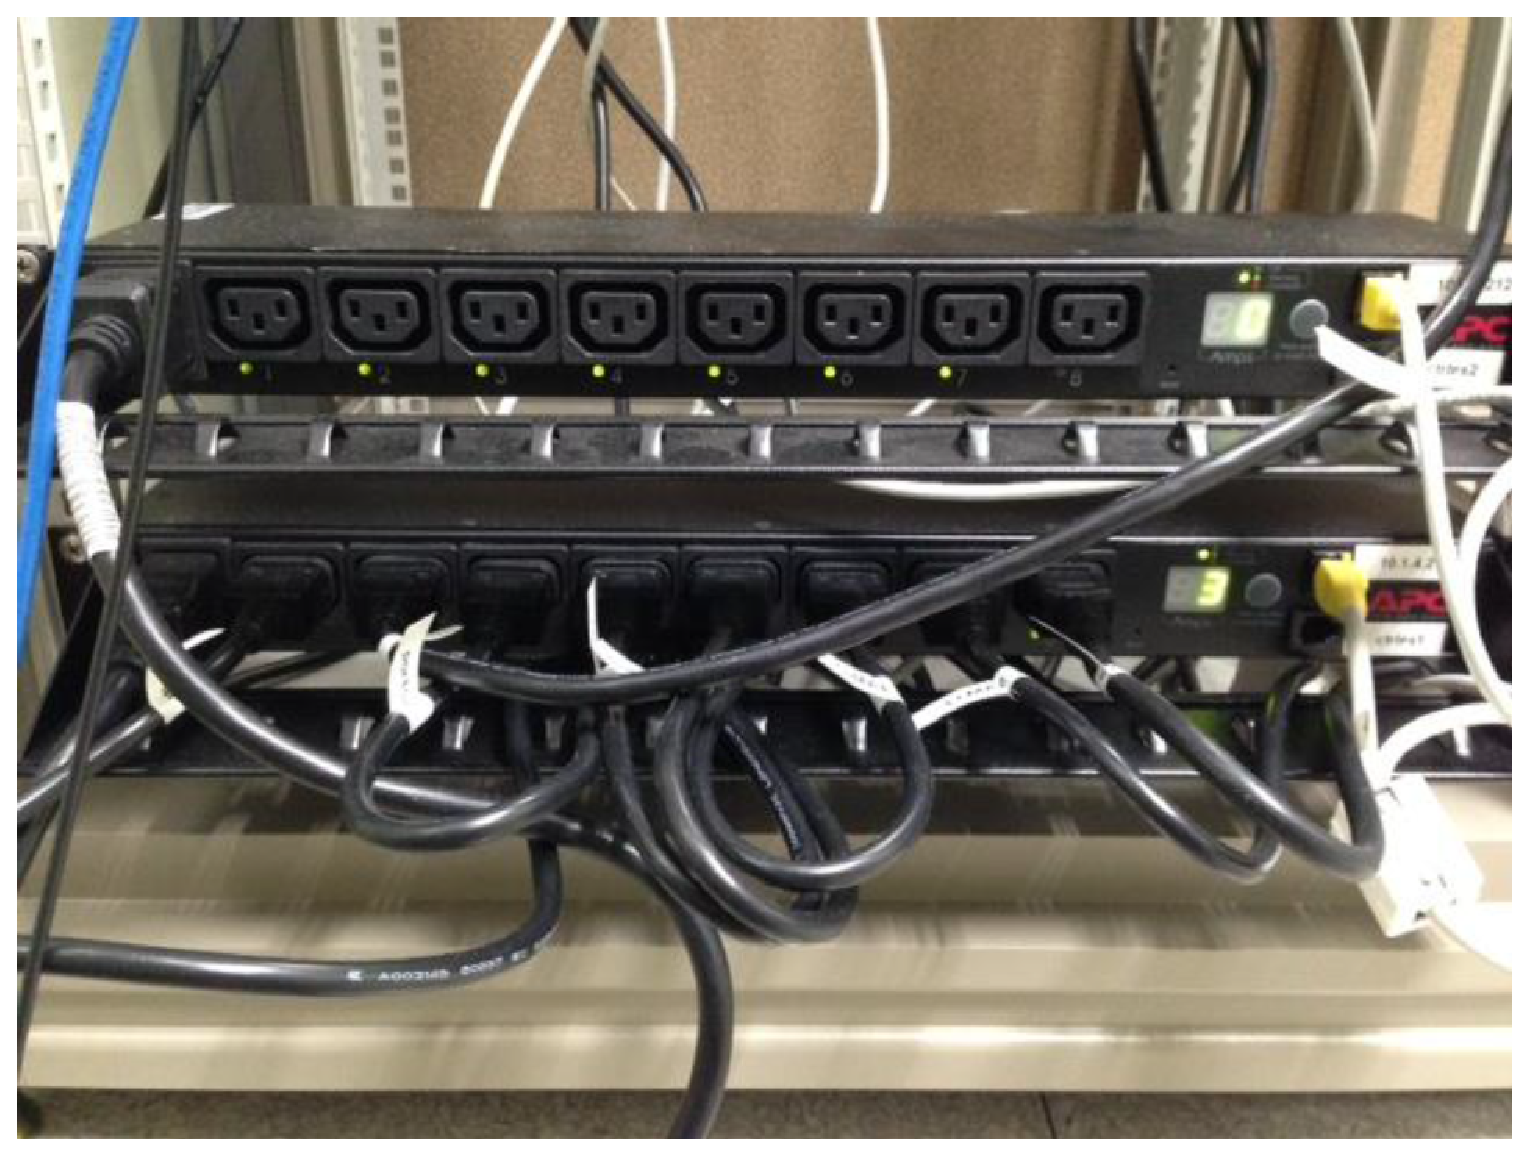
\includegraphics[width=0.6\textwidth]{./images/apc_pdu.eps}
  \caption{APC PDU}
  \label{fig:apc_pdu}   
\end{figure}

\begin{lstlisting}[style=termstyle, caption=APC PDU 모니터링 및 제어결과]]
mijoy0909@mjpark:~/users/mijoy0909$ ./powernet_test8.sh

*****************************
*          OPTIONS          *
*****************************
  [s] Status                 
  [1] ON                     
  [2] OFF                    
  [3] Reboot                 
  [4] On with delay          
  [5] Off with delay         
  [6] Reboot with delay      
  [q] Exit                   
  [0] Help                   
*****************************
-> Please enter your choice : 2

------------------------------------------------------------
 PowerWatts                      , 220
 Load Status                     , 1.0 Amps

   #       Name       Status      Control Outlet Command
============================================================
   1     "Outlet 1"      On              immediateOn
   2     "Outlet 2"      On              immediateOn
   3     "Outlet 3"      On              immediateOn
   4     "Outlet 4"      On              immediateOn
   5     "Outlet 5"      On              immediateOn
   6     "Outlet 6"      On              immediateOn
   7     "Outlet 7"      On              immediateOn
   8     "Outlet 8"      On              immediateOn
============================================================
------------------------------------------------------------
  [s] Status                 
  [1] Outlet1                
  [2] Outlet2                
  [3] Outlet3                
  [4] Outlet4                
  [5] Outlet5                
  [6] Outlet6                
  [7] Outlet7                
  [8] Outlet8                
  [b] Back                   
  [q] Exit                   
  [0] Help                   
-> Select outlet: 8
-> Are you sure? [y/n]y
outletOff

------------------------------------------------------------
 PowerWatts                      , 220
 Load Status                     , 1.0 Amps

   #       Name       Status      Control Outlet Command
============================================================
   1     "Outlet 1"      On              immediateOn
   2     "Outlet 2"      On              immediateOn
   3     "Outlet 3"      On              immediateOn
   4     "Outlet 4"      On              immediateOn
   5     "Outlet 5"      On              immediateOn
   6     "Outlet 6"      On              immediateOn
   7     "Outlet 7"      On              immediateOn
   8     "Outlet 8"     Off             immediateOff
============================================================
------------------------------------------------------------
\end{lstlisting}


\clearpage

\chapter{SNMP 응답시간 실험}
앞서 수행한 기본적인 연구와 다양한 Bash Shell Scripts 작성을 통해 SNMP는 버전별 응답시간의 차이가 있음을 알 수 있었다. 따라서 네트워크 토폴로지에서 장비가 놓이게 될 위치 선정과 원하는 장비의 응답시간 예측을 위해 스위치 개수와 케이블 길이에 따라 모니터링과 제어에 걸리는 SNMP 버전별 응답시간을 측정, 분석, 그리고 예측하고자 한다.

\section{실험 목적}
가속기 시설의 복잡성, 장비의 다양성, 그리고 안전한 접근성을 만족하며, 동시에 안정된 응답시간을 보장하는 장비의 설치 위치를 선정하는 것은 어려운 일이다. 따라서 사용자와 관리자, 혹은 시스템이 요구하는 응답시간과 보안 조건, 그리고 안정성 등을 고려한 제어 네트워크 토폴로지 설계 및 최적화가 필요하다. 이러한 설계와 최적화에 있어 필요한 물리적인 구성요소는 사용된 Layer2 스위치의 개수와 이를 연결하는 Ethernet 케이블의 길이이다. 그러므로 케이블 길이와 사용된 Layer2 스위치의 개수에 따른 장비의 응답시간 측정이 요구된다. 따라서 실험을 통해 얻게 되는 결과들은 네트워크 토폴로지 설계 및 장비의 최적화된 설치위치 선정에 도움이 될 것이다.

\section{선행실험}
선행실험은 암호화 및 복호화에 걸리는 시간, 케이블 딜레이, 하드웨어 자체의 속도, 사용한 Linux OS에 대한 응답시간의 차이가 같다는 가정에 따라 같은 케이블의 길이에서 snmpwalk 명령어를 이용해 장비의 특정 정보를 1,000번 요청하는 방식으로 수행되었다. 그림 \ref{fig:prestest}는 SNMP 버전 별 요청에 따른 응답시간의 평균과 편차를 나타낸 그래프로 SNMPv1/v2c는 서로 비교할 수 없는 오차 범위에 있으며, v3는 타 버전보다 1.5배 정도의 시간이 더 소모됨을 알 수 있다. 

\begin{figure}[!h]
  \centering
  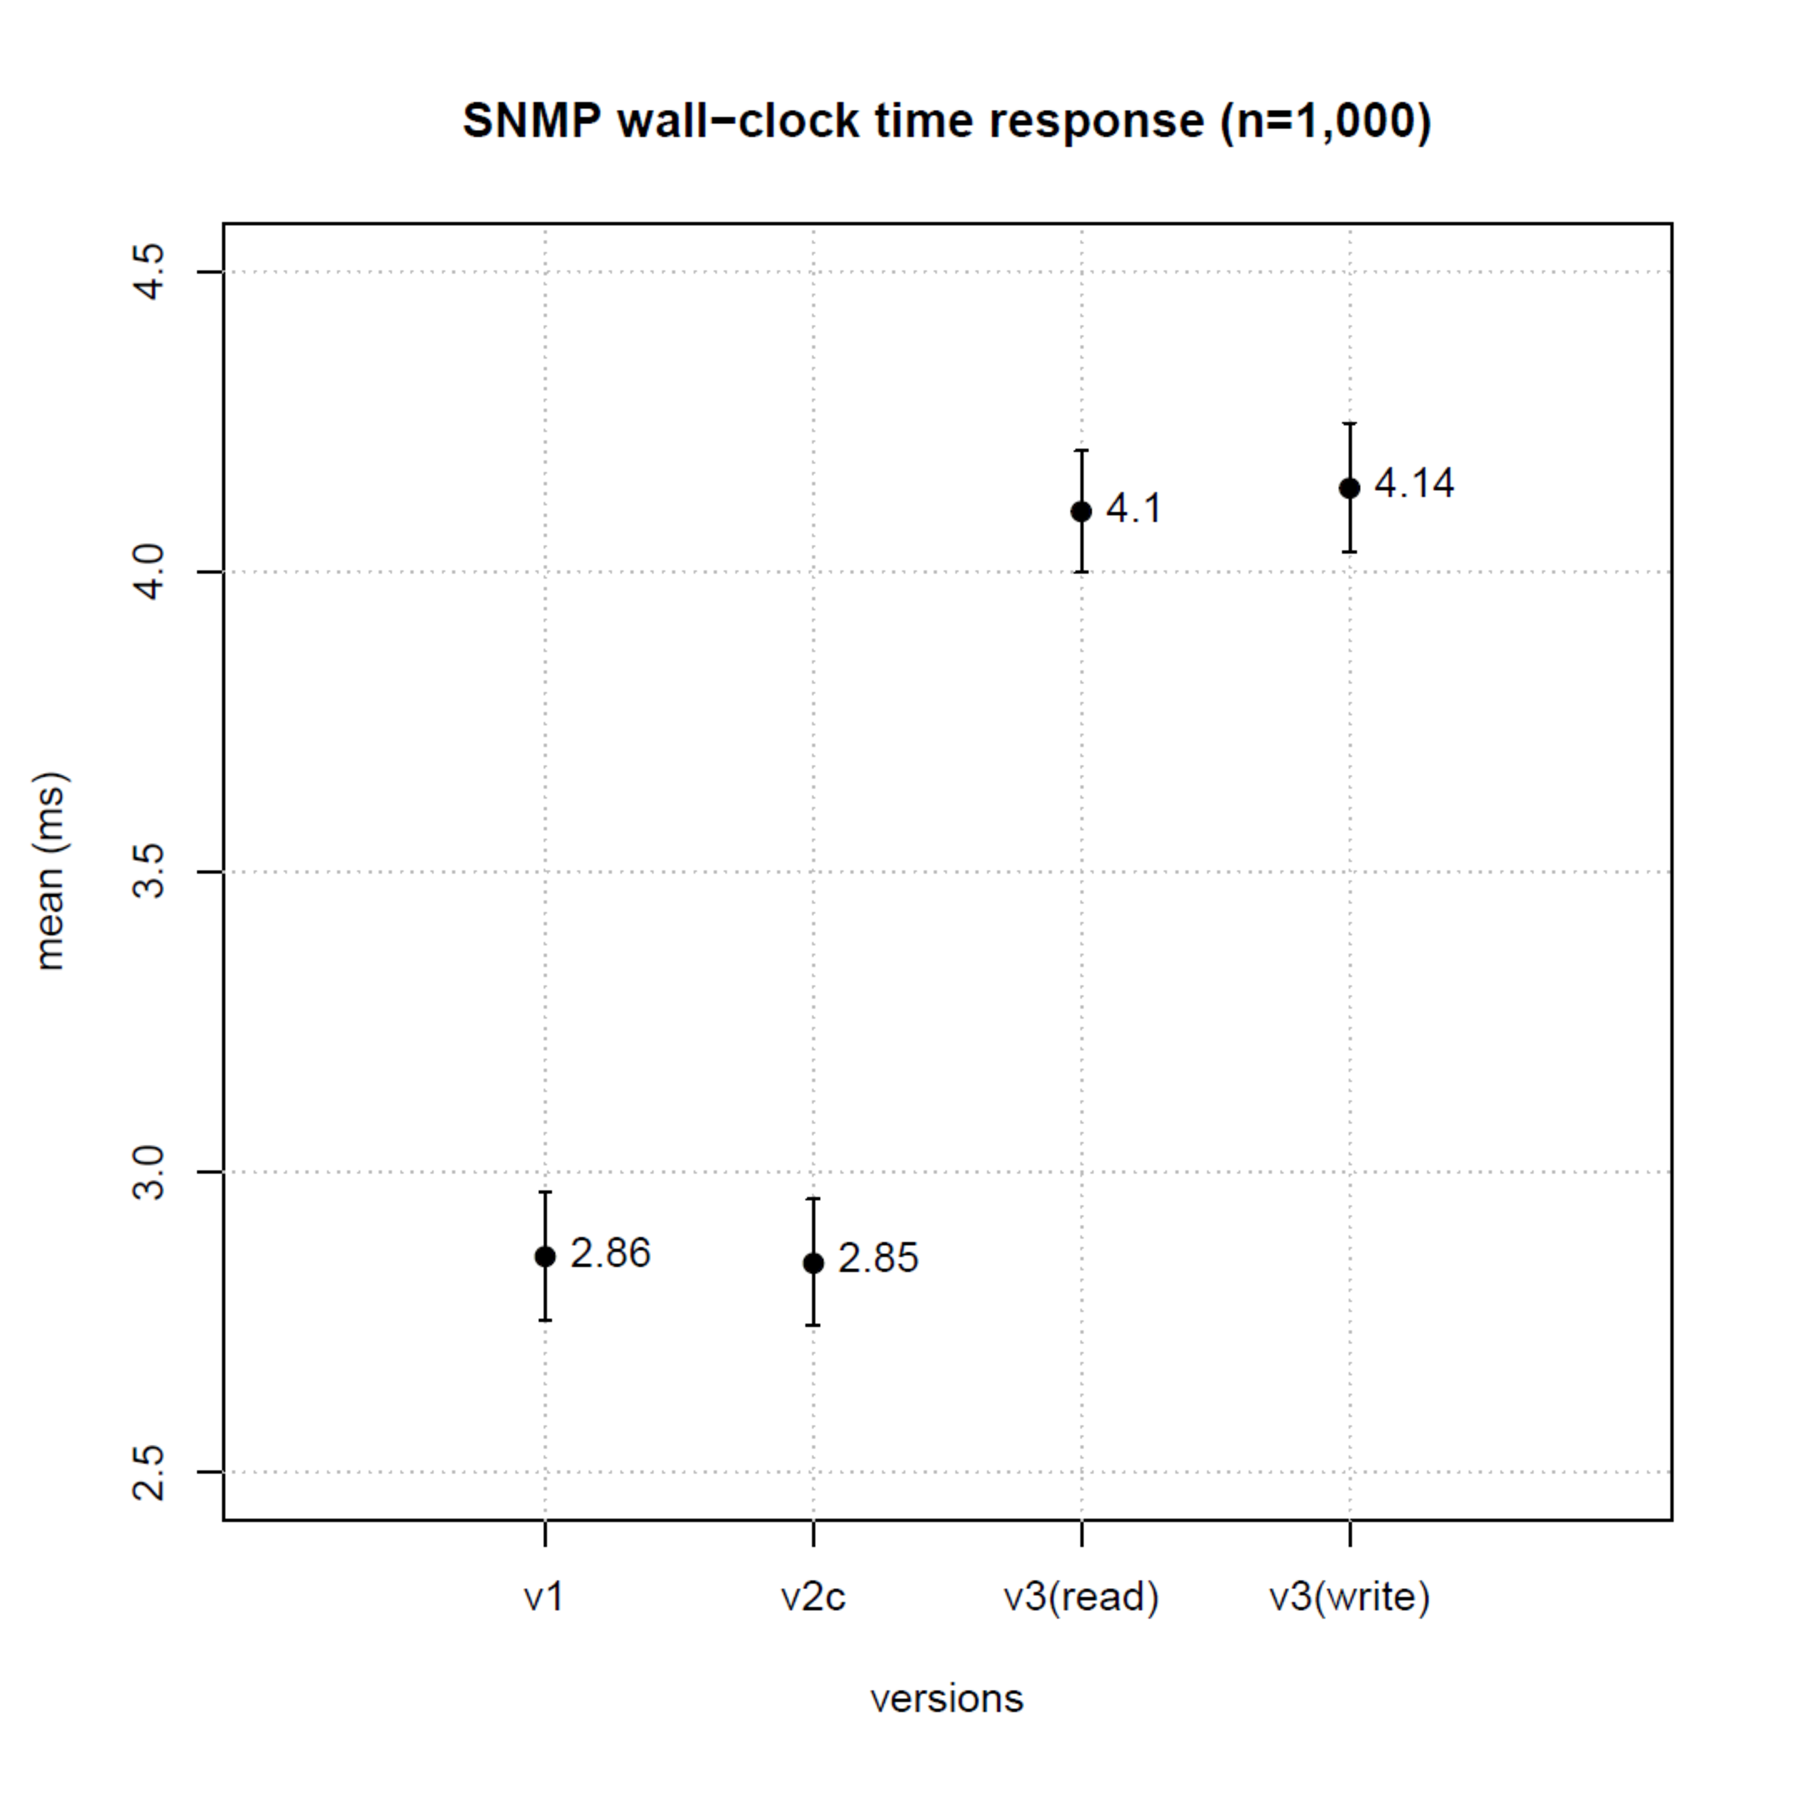
\includegraphics[width=0.9\textwidth]{./images/pretest.eps}
  \caption{SNMP 버전에 따른 응답시간의 차이}
  \label{fig:prestest}   
\end{figure}


\section{실험 방법}
본 실험에서는 프로그램이 수행되는 시간을 측정하는 리눅스의 time 명령어\citep{time_command}를 이용하여 Bash Shell Script 수행에 걸리는 시간을 응답시간으로 측정하였다. time 명령어는 아래와 같이 세 가지 형태의 시간 측정 결과를 나타낸다. 
\begin{itemize}
\item real : 실제로 걸린 시간
\item user : 커널이 사용한 시간을 제외한 CPU에서 소비된 시간
\item sys : 실제로 할애한 커널 시간
\end{itemize}
이를 참조하면 user+sys 시간은 실제로 작업에 할애된 시간이며, real-(user+sys) 시간은 다른 프로세서 처리에 할당된 시간이다. 따라서 본 실험에서는 Layer 2 스위치 간의 내부 시간 차이와 Ethernet 케이블 제작 시 발생하는 길이의 오차 등에서 발생하는 시간이 포함된 실제 작업 시간인 user+sys 시간을 사용한다. 일반적으로 가장 많이 사용하는 Ethernet UTP 케이블이 물리적 신호를 안정적으로 전달할 수 있는 최대 길이가 100m인 점을 고려하여 본 실험에는 1, 10, 20, 30, 40, 50, 100m 길이의 Category6 케이블을 사용한다. 또한, 실험에 사용된 소프트웨어 및 하드웨어는 아래와 같다.

\begin{itemize}
\item Debian Linux 7 Wheezy
\item NET-SNMP v5.4.3
\item R v2.15.1
\item GNU Bash Script-CLI(Command-line Interface) 
\item Switch(BROCADE ICX6430)
\item Power Distribution Unit(APC PDU 7921)
\end{itemize}

\subsection{3.2.1 Bash Script 구성}
본 문서의 SNMPv1/v2c/v3의 응답시간 측정에는 GNU Bash Shell을 이용하여 만든 Script를 사용한다. 이는 APPENDIX A를 참고 바란다. Script는 그림 \ref{fig:shellscript}과 같이 v1/2c일 경우 snmpget 명령어로 PDU Outlet 8번의 상태 정보를 1,000번 요청하고, v3의 경우 상태 정보 요청뿐만 아니라 snmpset 명령어로 Outlet 8번의 전원을 켜는 명령어 1,000번 수행하도록 구성되었다. 구성된 Script는 리눅스 Sleep 명령어를 사용해 1초 멈추는 조건과 그렇지 않은 조건으로 나뉘어 수행되고 time 명령어를 사용해 이 과정에 걸린 시간을 측정한다. 측정결과는 계산되어 CLI에 total count, mean, sample deviation, standard deviation으로 표현된다. 

\begin{figure}[!htb]
  \centering
  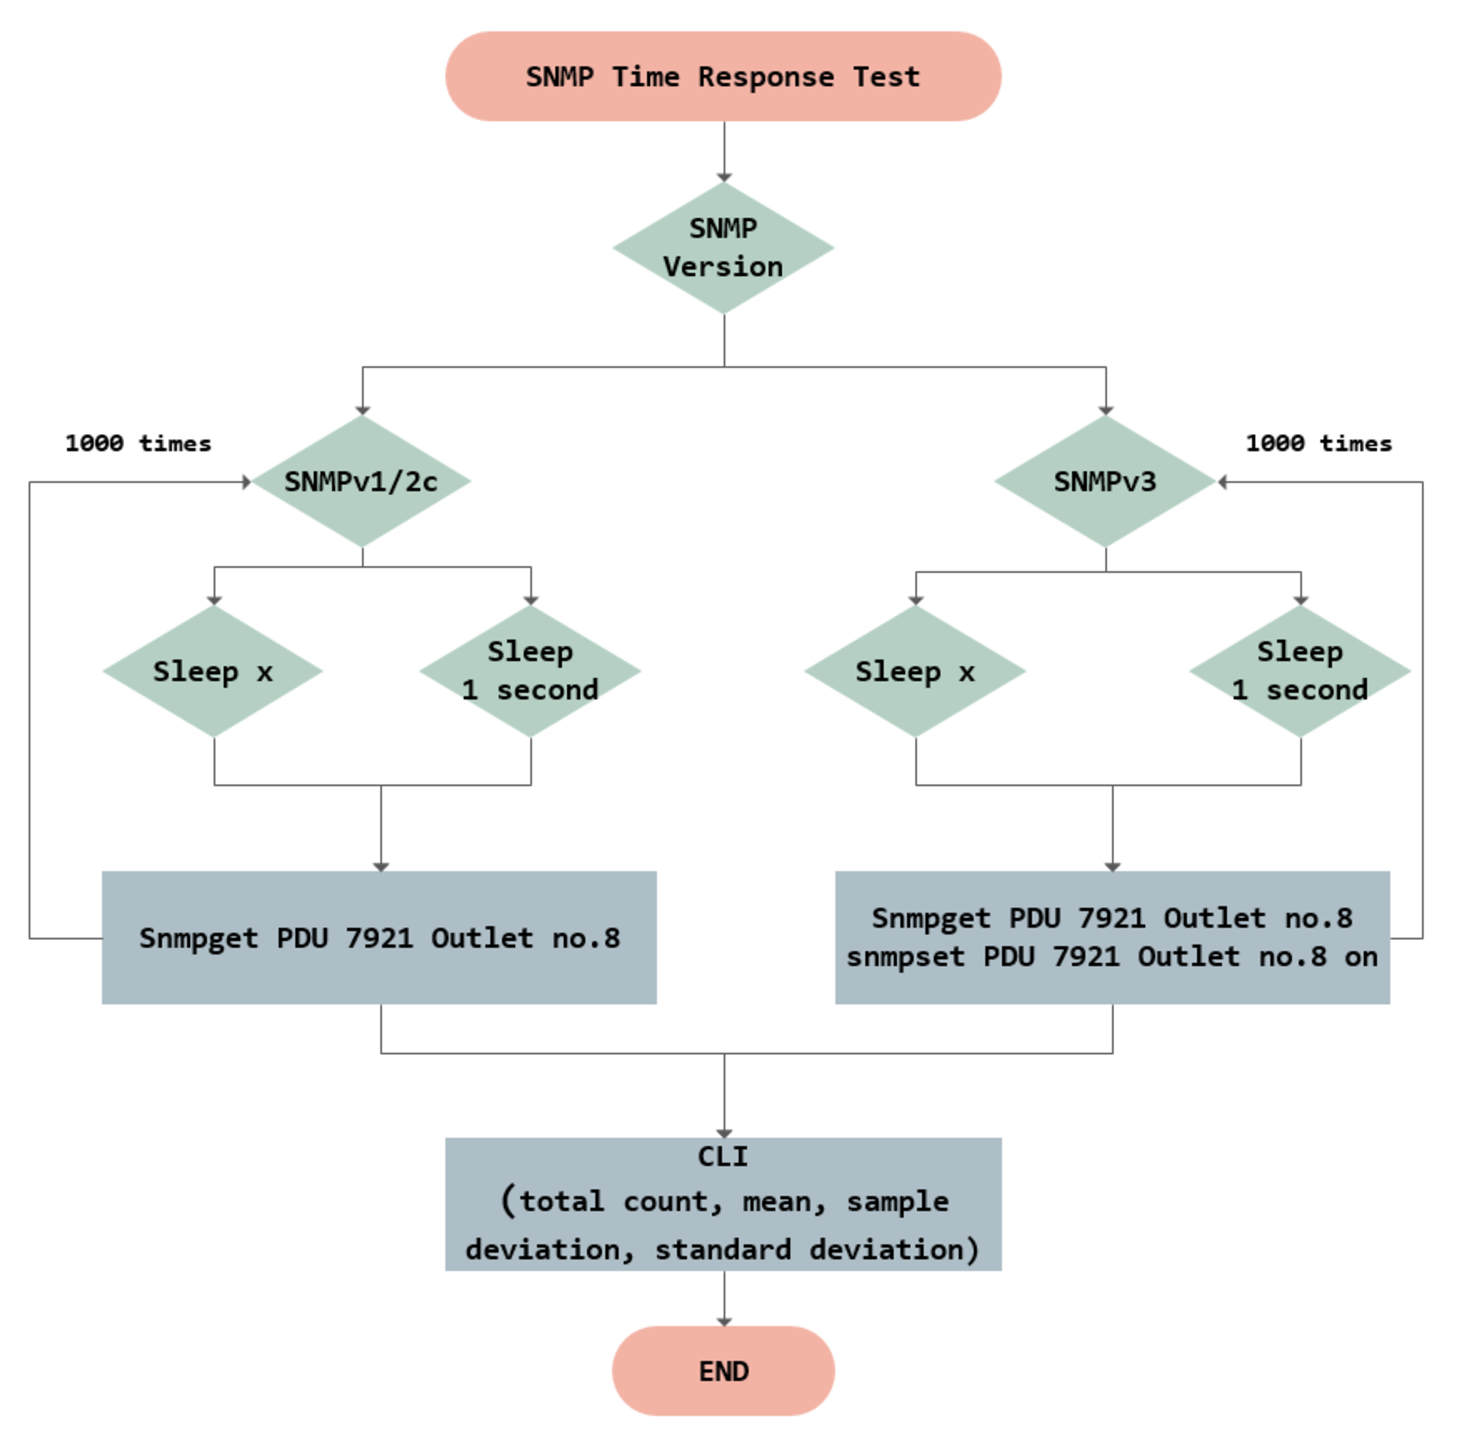
\includegraphics[width=0.9\textwidth]{./images/bashshelscript.eps}
  \caption{Bash Shell Script 순서도 }
  \label{fig:shellscript}   
\end{figure}

\subsection{3.2.2 실험 환경 및 방법}
실험은 그림 \ref{fig:switch5}의 배치도와 같이 구성하여 케이블 길이와 스위치 개수를 변경하면서 Bash Script의 실행으로 진행된다.

\begin{figure}[!htb]
  \centering
  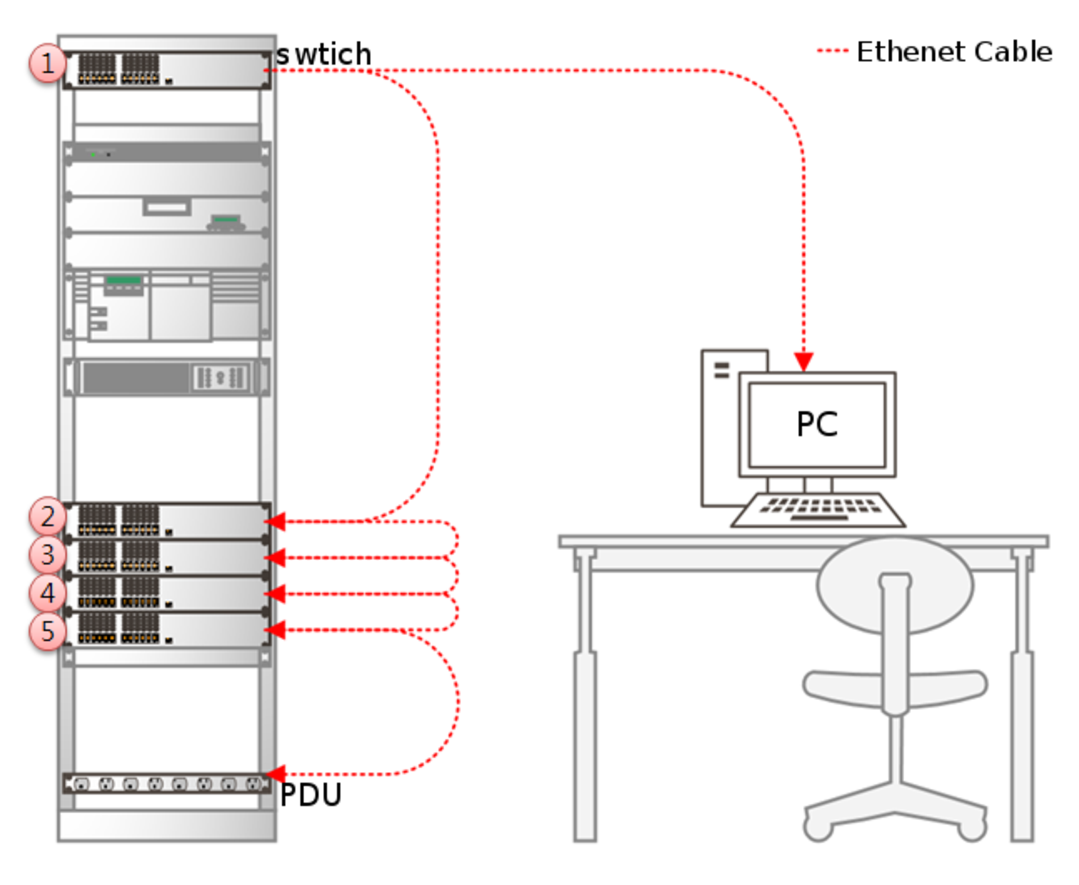
\includegraphics[width=0.9\textwidth]{./images/switch5.eps}
  \caption{실험 배치도 (스위치 5개 일 때)}
  \label{fig:switch5}   
\end{figure}

\clearpage

- 실험방법 \par

1. 컴퓨터와 스위치를 측정하고자 하는 길이의 케이블로 연결한다.\par
2. Bash Script에서 응답시간 측정 옵션을 선택한다.\par
3. 실험환경에 따라 옵션을 선택한 후 log 파일의 이름을 정의한다.\par
4. 1~3의 과정을 1, 50, 100m의 케이블과 스위치 개수를 변경하면서 반복 수행한다. 이때 그림 \ref{fig:devcon}와 같이 컴퓨터는 첫 번째 스위치에 계속 연결되어있고, PDU는 추가되는 스위치에 연결한다. \par

\begin{figure}[!htb]
  \centering
  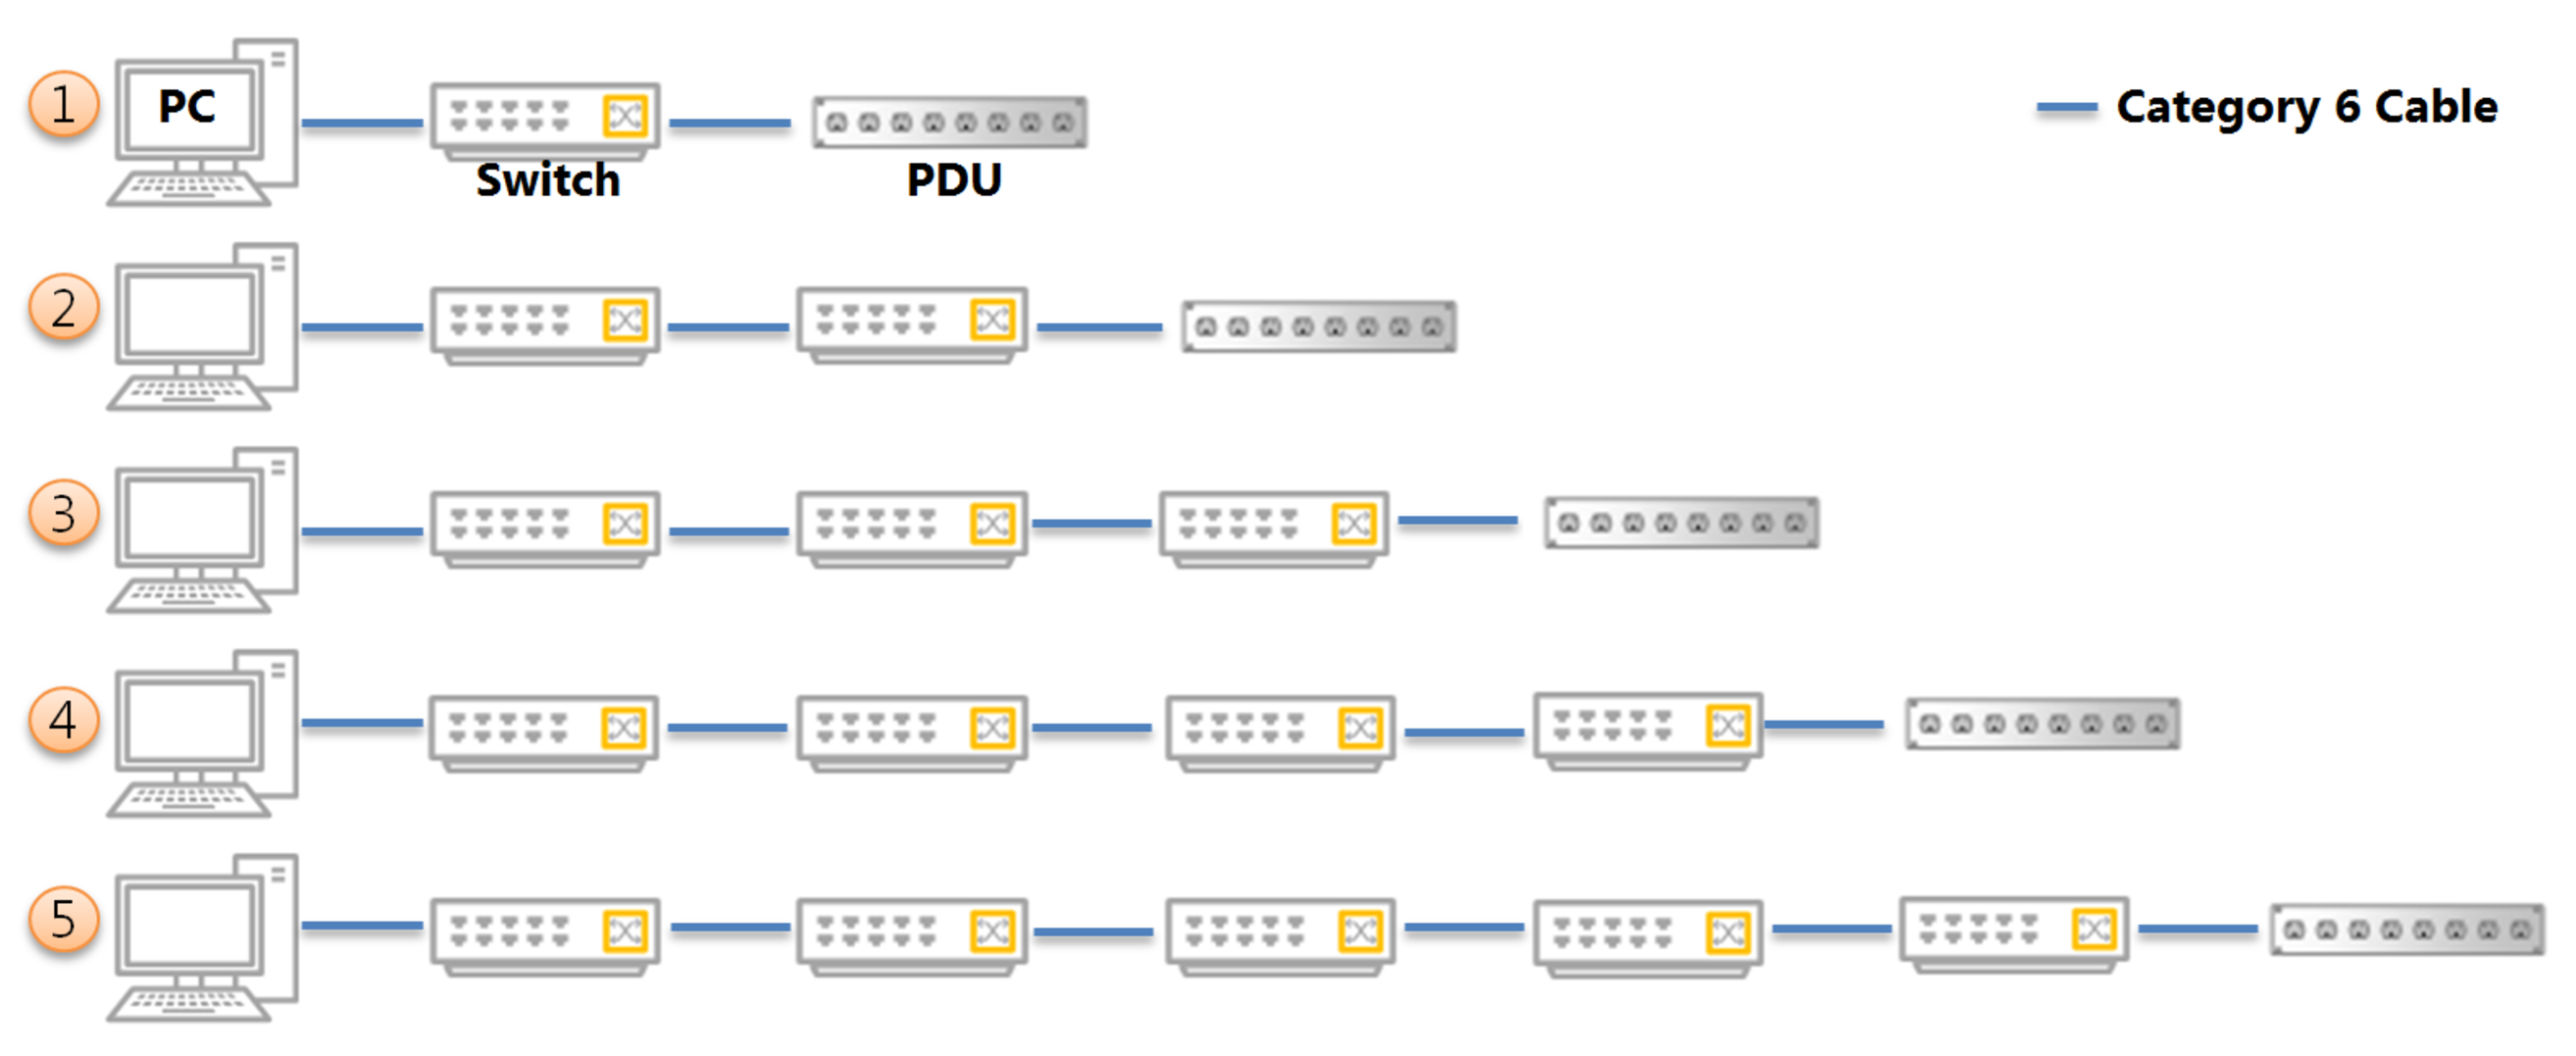
\includegraphics[width=0.9\textwidth]{./images/deviceconnet.eps}
  \caption{장비 연결 구성도}
  \label{fig:devcon}   
\end{figure}

5. Script의 File Merge 옵션으로 ASCII 파일로 저장된 응답시간의 mean 값 데이터를 그림 \ref{fig:time_table}과 같은 테이블로 재구성한다. \par
6. R로 1, 50, 100m의 응답시간 데이터를 사용해 10, 20, 30, 40m 케이블 길이에서의 응답시간을 예측한다.\par
7. 1~5 과정으로 10, 20, 30, 40m 케이블에서의 응답시간을 측정한다.\par
8. 측정값과 예측된 값을 비교하고 회귀분석을 통해 가설을 검증한다.\par

\begin{figure}[!htb]
  \centering
  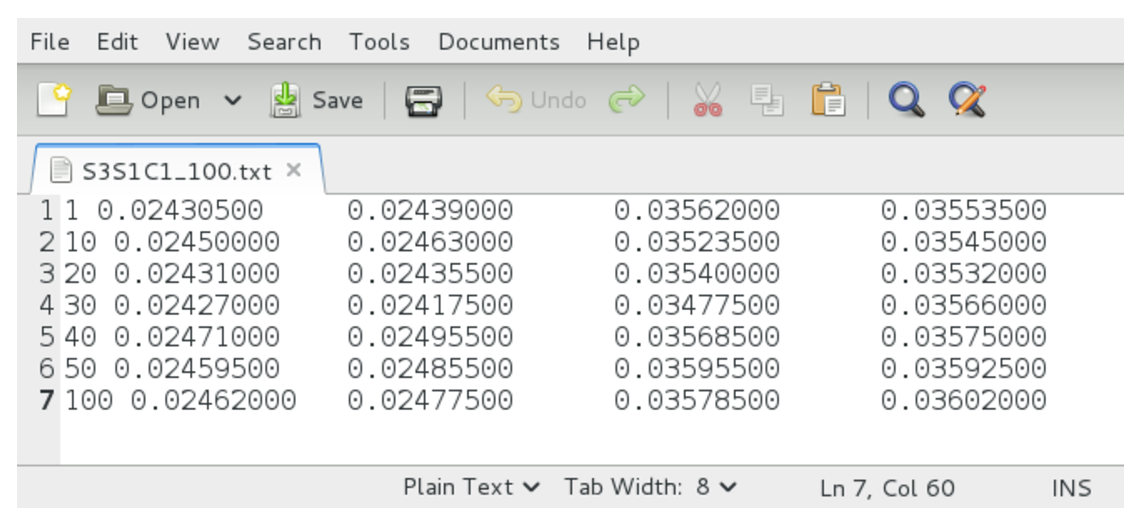
\includegraphics[width=0.8\textwidth]{./images/timetable.eps}
  \caption{데이터 테이블}
  \label{fig:time_table}   
\end{figure}

\clearpage
\section{실험 결과}
\subsection{3.4.1 스위치 개수, 케이블 길이와 응답시간의 관계}
본 장에서는 실험에 앞서 스위치 개수와 케이블 길이가 응답시간에 영향을 미칠 것으로 생각했다. 따라서 스위치 개수, 케이블 길이와 응답시간 간의 관련성이 연구할 만한 자료인지 판단하기 위해 표 \ref{table:s1}의 Sleep을 1초한 응답시간의 평균값을 사용하였다. 

\begin{table}[!htb]
\begin{center}
\begin{tabular}{c|c|c|c|c|c|c}\hline
 & Version & Switch1 & Switch2 & Switch3 & Switch4 & Switch5\\ \hline
1m & v1 & 24.35 & 24.45 & 24.30 & 24.41& 24.50 \\ 
& v2c & 24.37 & 24.42 & 24.39 & 24.37 & 24.46 \\ 
& v3r & 35.78 & 35.56 & 35.62 & 35.70 & 35.60 \\ 
& v3w & 35.54 & 35.53 & 35.53 & 35.47& 35.37 \\\hline
50m & v1 & 24.73 & 24.66 & 24.59 & 24.89& 24.93 \\ 
& v2c & 24.83 & 24.73 & 24.85 & 24.73 & 24.75 \\ 
& v3r & 35.77 & 35.72 & 35.95 & 35.85 & 35.73 \\ 
& v3w & 35.54 & 35.53 & 35.53 & 35.47& 35.37 \\\hline
100m & v1 & 24.90 & 24.62 & 24.62 & 24.50& 24.37 \\ 
& v2c & 24.87 & 24.69 & 24.77 & 24.80 & 24.52 \\ 
& v3r & 35.85 & 35.86 & 35.78 & 35.92 & 35.52 \\ 
& v3w & 35.73 & 35.86 & 36.02 & 35.73& 35.59 \\\hline \hline
\end{tabular}
\caption{SNMP 버전별 응답시간의 평균값 (Sleep 1s) (단위 : ms)}
  \label{table:s1}  
\end{center}
\end{table} 

이를 통계 계산과 그래픽을 위한 프로그래밍 언어이자 소프트웨어 환경인 R로 linear fitting을 하고 linear그래프와 산점도를 그려 변수들의 상관관계를 확인하였다. 그림 \ref{fig:3ps1}의 그래프는 그 결과로 스위치의 개수 증가에 따른 SNMP 버전별 응답시간의 변화는 미미하고, 스위치의 개수가 5개까지 연결되었을 때 몇몇의 응답시간은 오히려 감소함을 알 수 있다. 그러나 케이블 길이 변화에 대한 응답시간은 대부분 증가함을 알 수 있다. non-sleep 환경에서의 실험 결과는 APPENDIX A를 참고 바란다.


\begin{figure}[!htb]
  \centering
  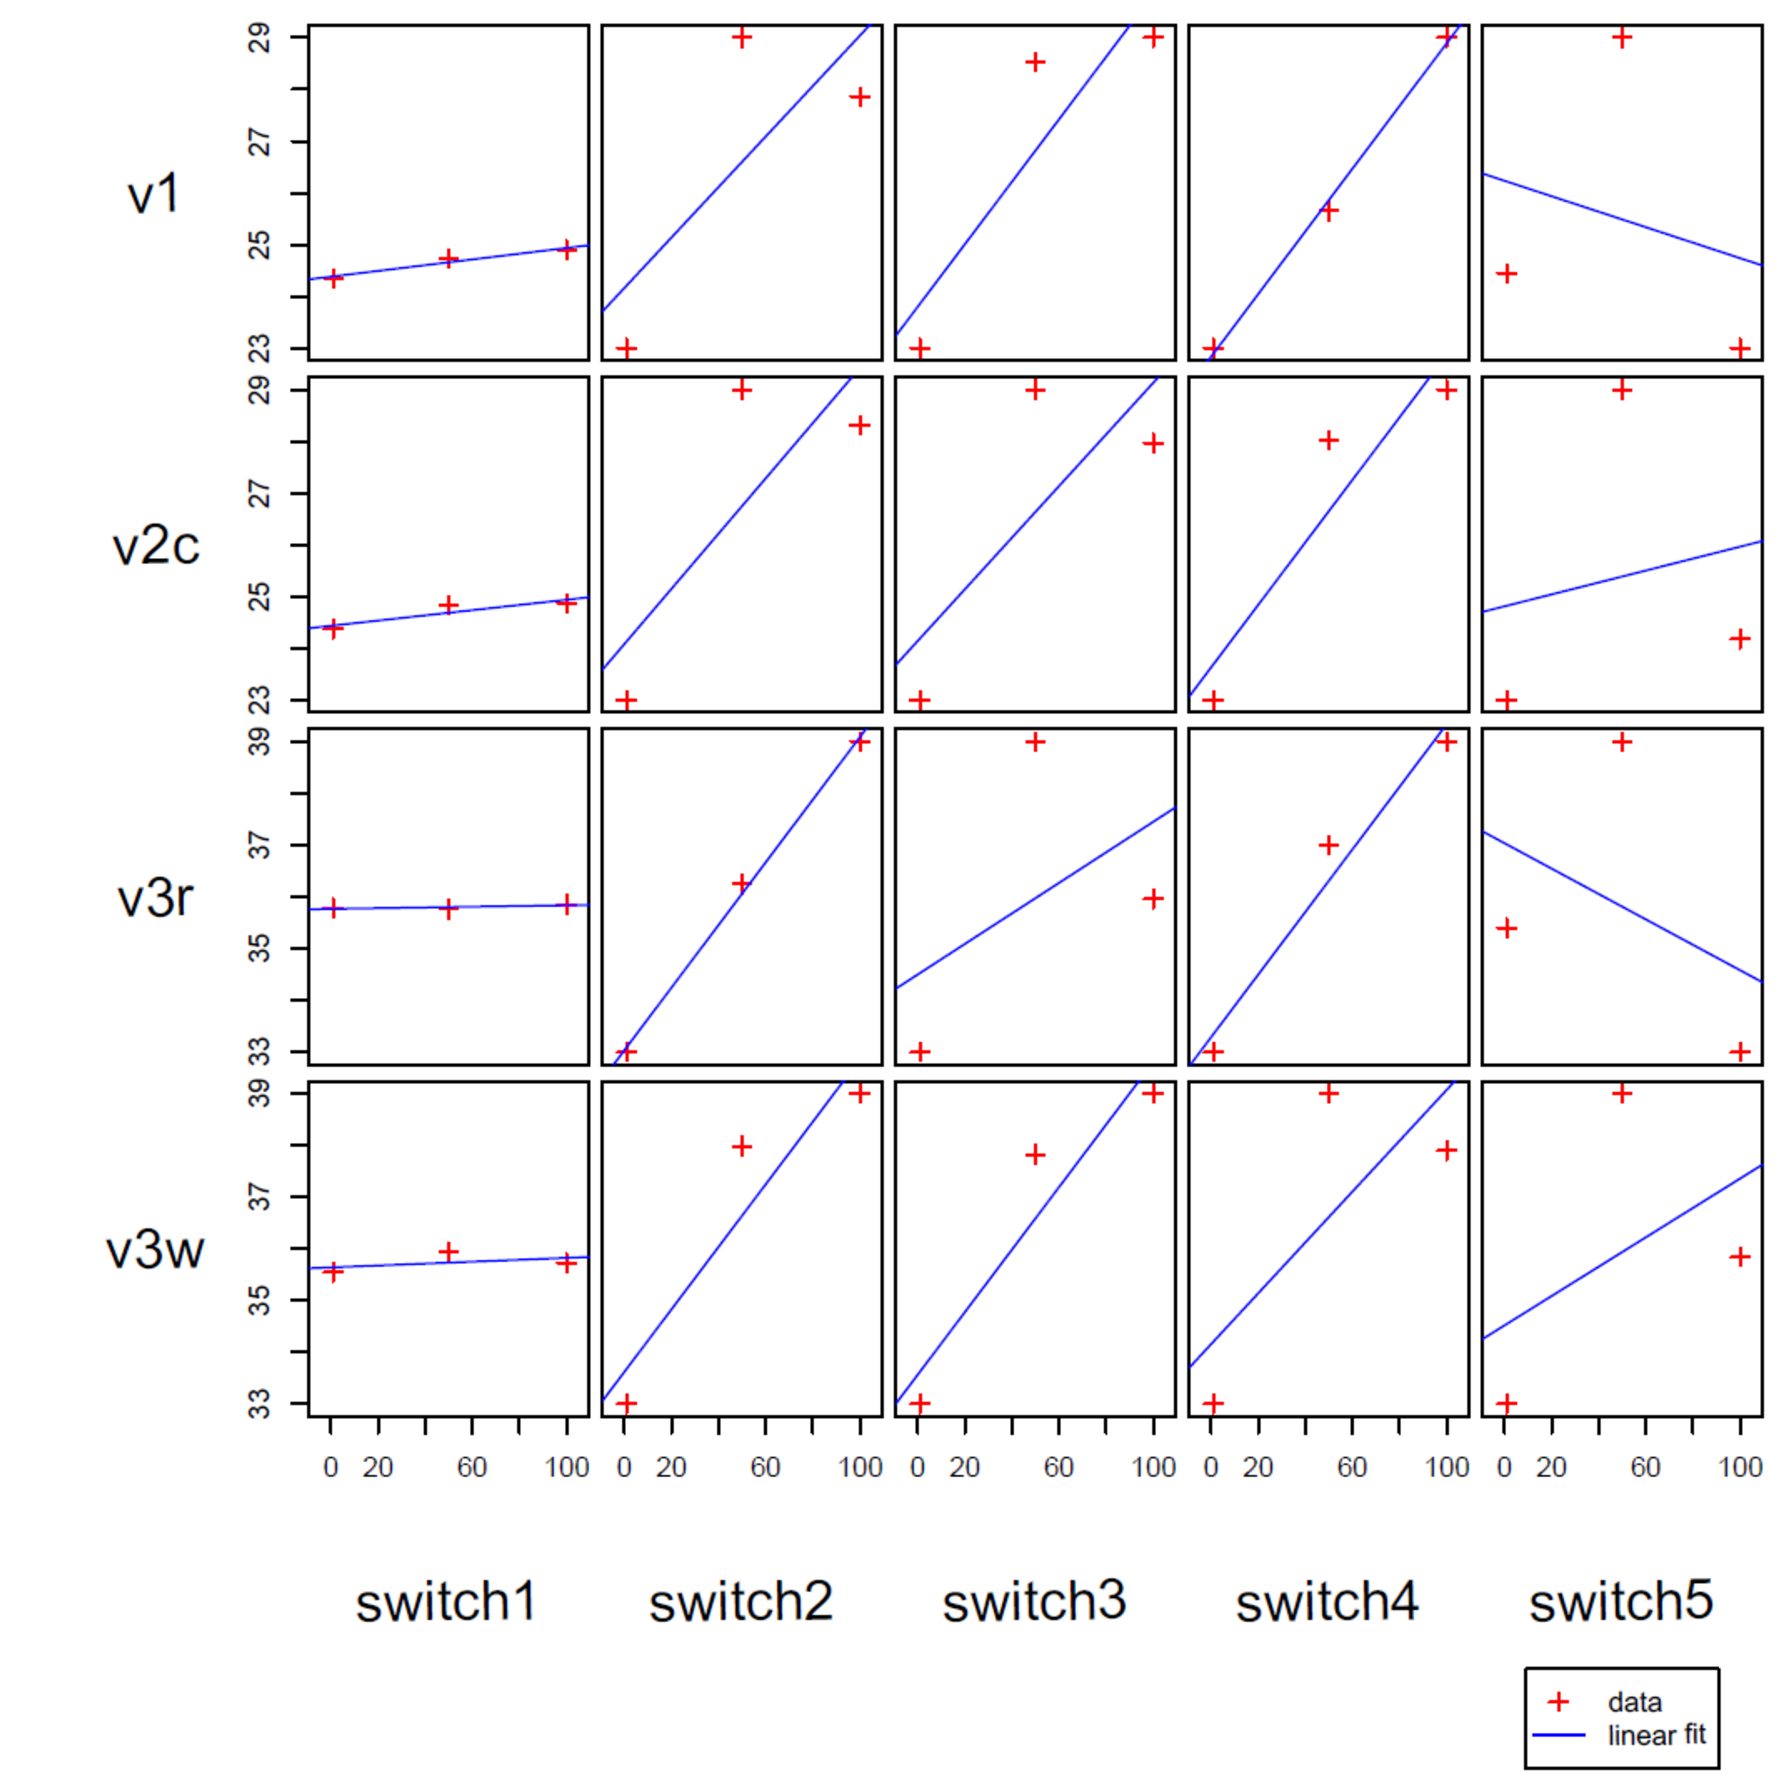
\includegraphics[width=0.9\textwidth]{./images/3point_sleep1s.eps}
  \caption{3-point 산점도와 linear그래프 (Sleep 1s)}
  \label{fig:3ps1}   
\end{figure}

\clearpage

\subsection{3.4.2 R을 통한 데이터 분석 및 예측}
데이터 분석에는 하나 또는 그 이상의 독립변수(a)의 종속변수(b)에 대한 영향의 추정을 할 수 있는 통계기법인 회귀분석을 사용한다\citep{analysis}. 회귀분석은 최소 하나 이상의 독립변수 값에 근거하여 종속변수 값을 예측하거나 독립변수가 종속변수에 미치는 영향력의 크기를 설명하는 데 유용하다. 회귀분석에서 독립변수는 다른 변수에 영향을 미치는 변수이고, 종속변수는 독립변수에 의해 영향을 받는 변수이다. 회귀분석에는 통계프로그래밍 언어인 R을 사용하며, 변수의 개수에 따라 단순회귀분석과 다중회귀분석을 수행한다.
\subsubsection{3.3.2.1 단순회귀분석}
먼저 독립변수를 케이블 길이(l)로 정하고, 종속변수인 응답시간(t)과의 관계를 단순회귀분석을 통해 확인하였다. 이를 나타내는 방정식은 회귀모델이며, 단순회귀모델은 식 \ref{eq:eps}과 같다. 

\begin{equation} \label{eq:eps}
  t=\alpha l + \beta  
\end{equation}

아래의 식 \ref{eq:eps2}는 회귀분석을 통해 구한 회귀식이다. 

\begin{equation} \label{eq:eps2}
  t=0.006537\alpha + 35.429898  
\end{equation}
\\
그림 \ref{fig:s3s1}는 스위치를 세 개 연결된 상태에서 Sleep 1초 실험환경에서 SNMPv2c와 v3w의 단순회귀분석그래프이다. 이 그래프에서 ●는 1, 50, 100m의 케이블 길이에서 측정한 응답시간, ×는 1, 50, 100m 길이에서의 측정한 응답시간을 R의 linear fitting 피팅을 통해 10, 20, 30, 40m의 길이에서 응답시간을 예측한 값이며, ▲는 10, 20, 30, 40m의 길이에서 실제 응답시간을 측정한 값이다. Confidence limit(녹색 점선)은 추가적인 실험 진행 시 1, 10, 20, 30, 40, 50, 100m의 케이블 길이에서 나올 수 있는 응답시간의 범위를 나타낸다. Prediction limit(청색 점선)은 실험에 사용된 케이블 길이가 아닌 길이의 케이블을 사용하여 응답시간 측정 시에 나올 수 있는 응답시간의 범위이다. 따라서 중요한 장비, 즉 정해진 응답시간이 필요한 장비들은 이를 고려한 네트워크 설계가 이루어져야 한다. 

\begin{figure}[!h]
  \centering
  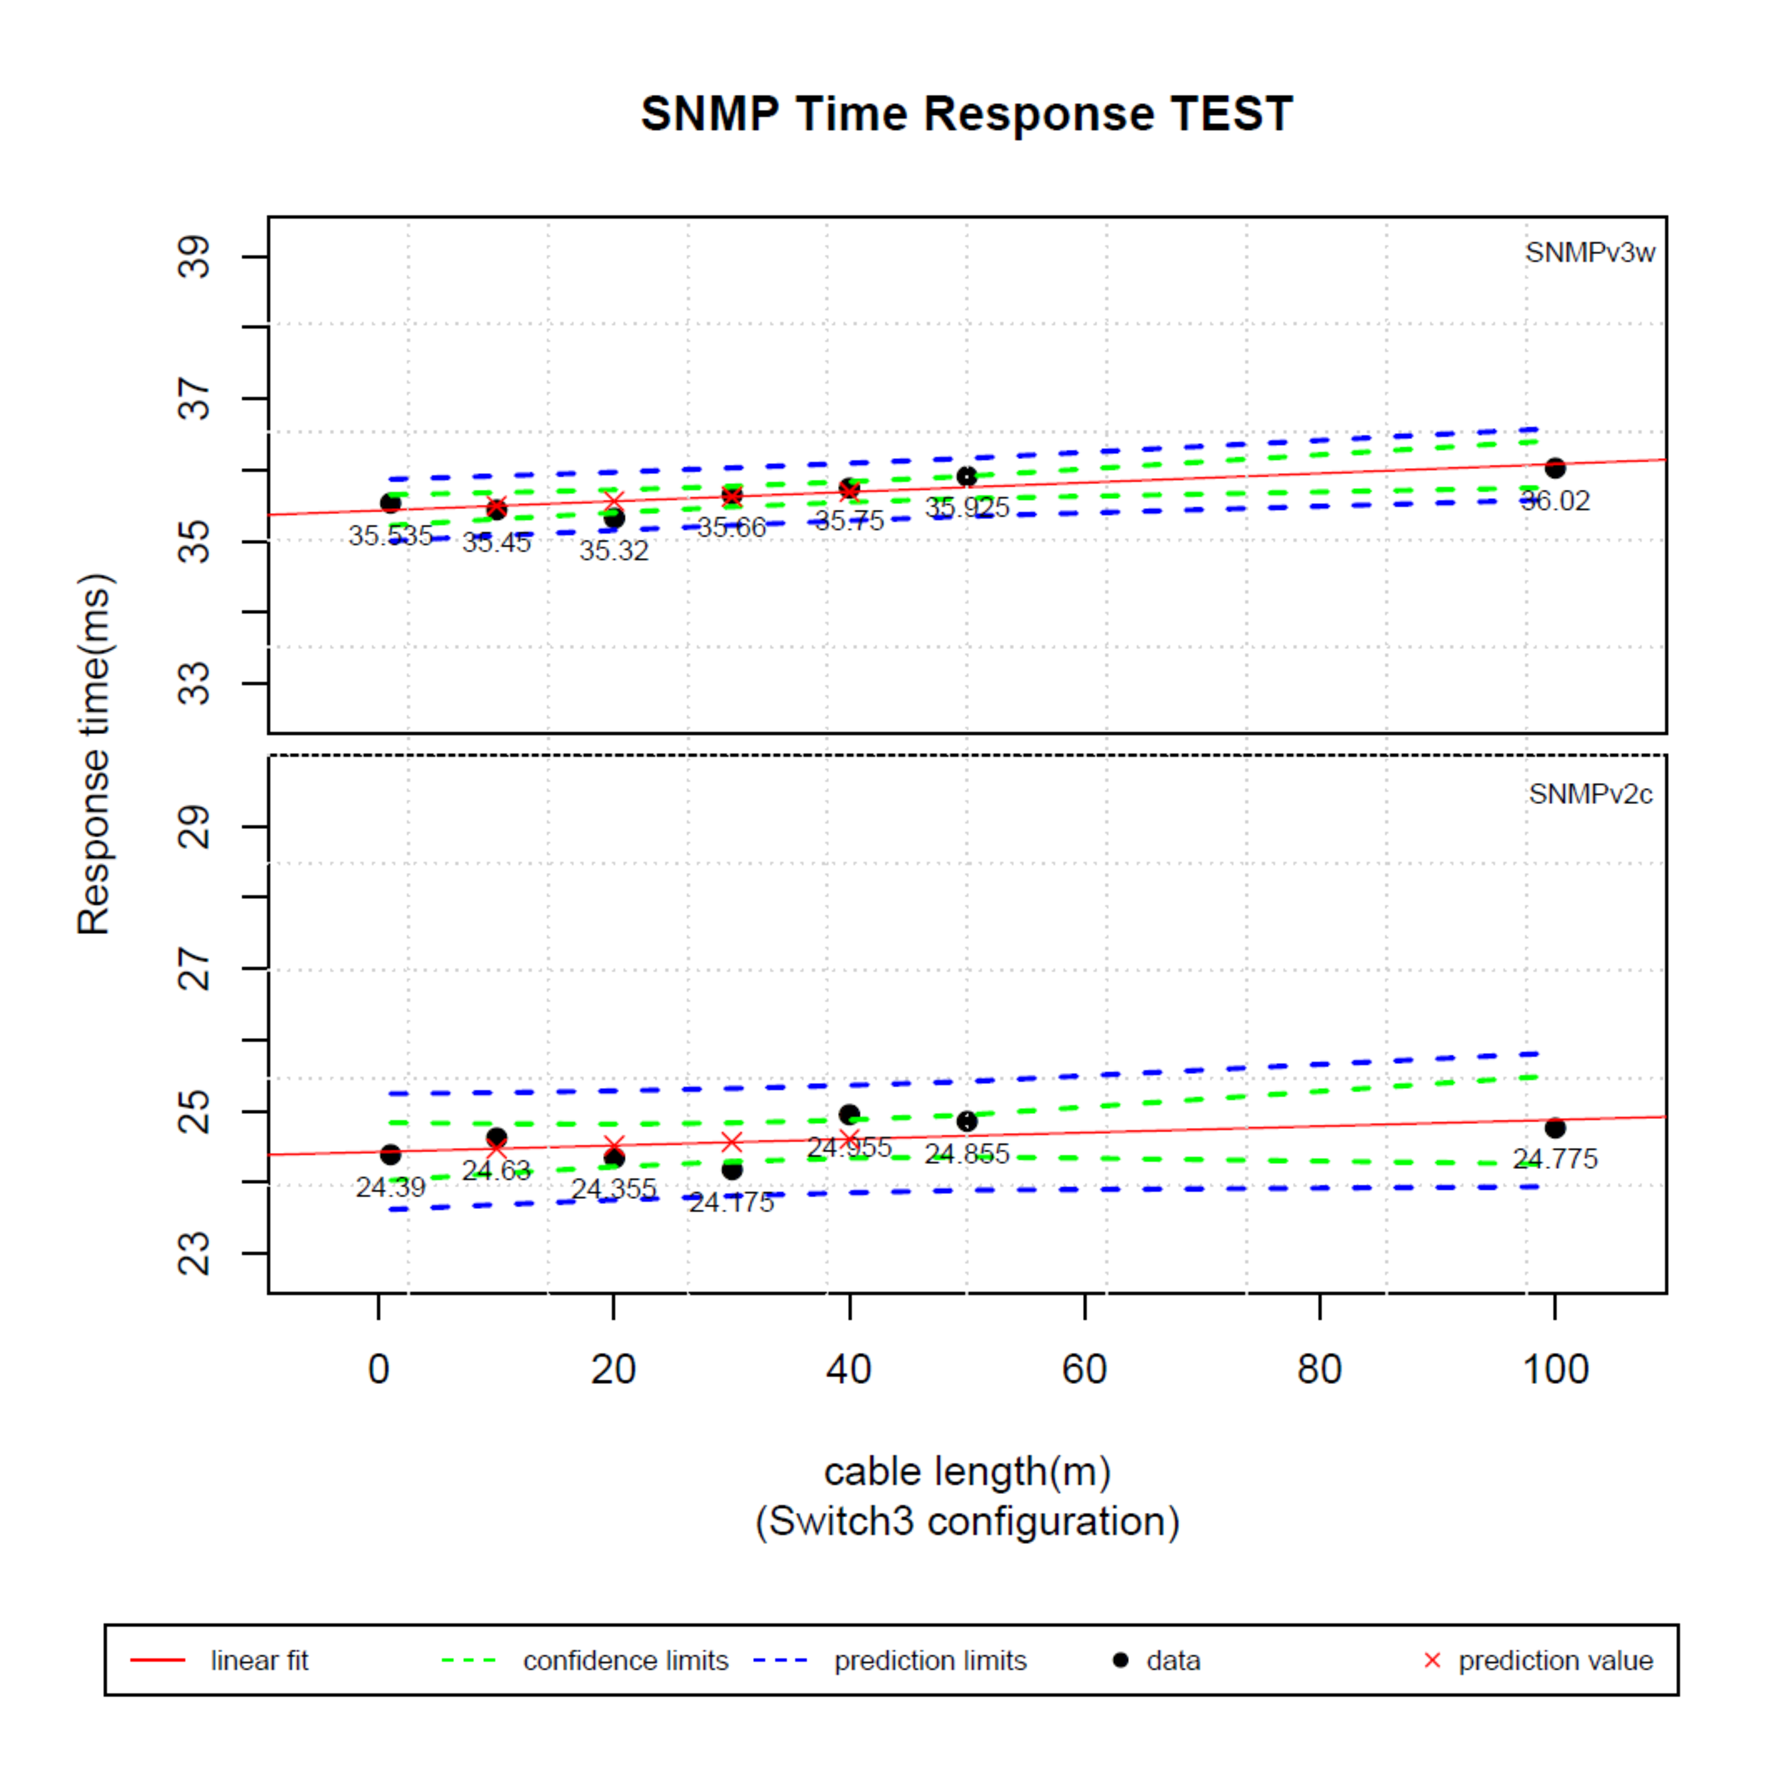
\includegraphics[width=0.88\textwidth]{./images/s3s1.eps}
  \caption{회귀분석 그래프(스위치 3개/Sleep1)}
  \label{fig:s3s1}   
\end{figure}


\begin{table}[!b]
\begin{center}
\begin{tabular}{c|c|c|c|c}\hline
길이(m) & 10 & 20 & 30 & 40 \\ \hline
예측응답시간(ms)& 35.50 & 35.56 & 35.63 & 35.69 \\ \hline
실제응답시간(ms)& 35.45 & 35.32 & 35.75 & 36.02 \\ \hline
\end{tabular}
\caption{케이블 길이에 따른 응답시간의 예측과 측정(v3w)}
  \label{table:predict_time}  
\end{center}
\end{table} 

표 \ref{table:predict_time}는 그림 \ref{fig:s3s1}에서  v3w 부분을 표식 화한 것으로, 실험 결과 예측된 응답시간과 실제 측정한 응답시간이 ±1ms의 오차범위 내에 있는 것을 확인할 수 있다. 이를 바탕으로 그림 \ref{fig:7ps1}과 같이  스위치의 개수와 측정한 모든 케이블 길이에서의 응답시간에 관한 산점도와 linear그래프를 그려 변수들의 상관관계를 재확인하였다. 이는 그림 \ref{fig:3ps1}의 결과와 마찬가지로 스위치 개수의 증가에 비해 케이블 길이의 변화가 응답시간에 더 영향을 미치는 것을 알 수 있다. 다른 환경에서의 실험 결과는 APPENDIX A를 참고 바란다.

\begin{figure}[!h]
  \centering
  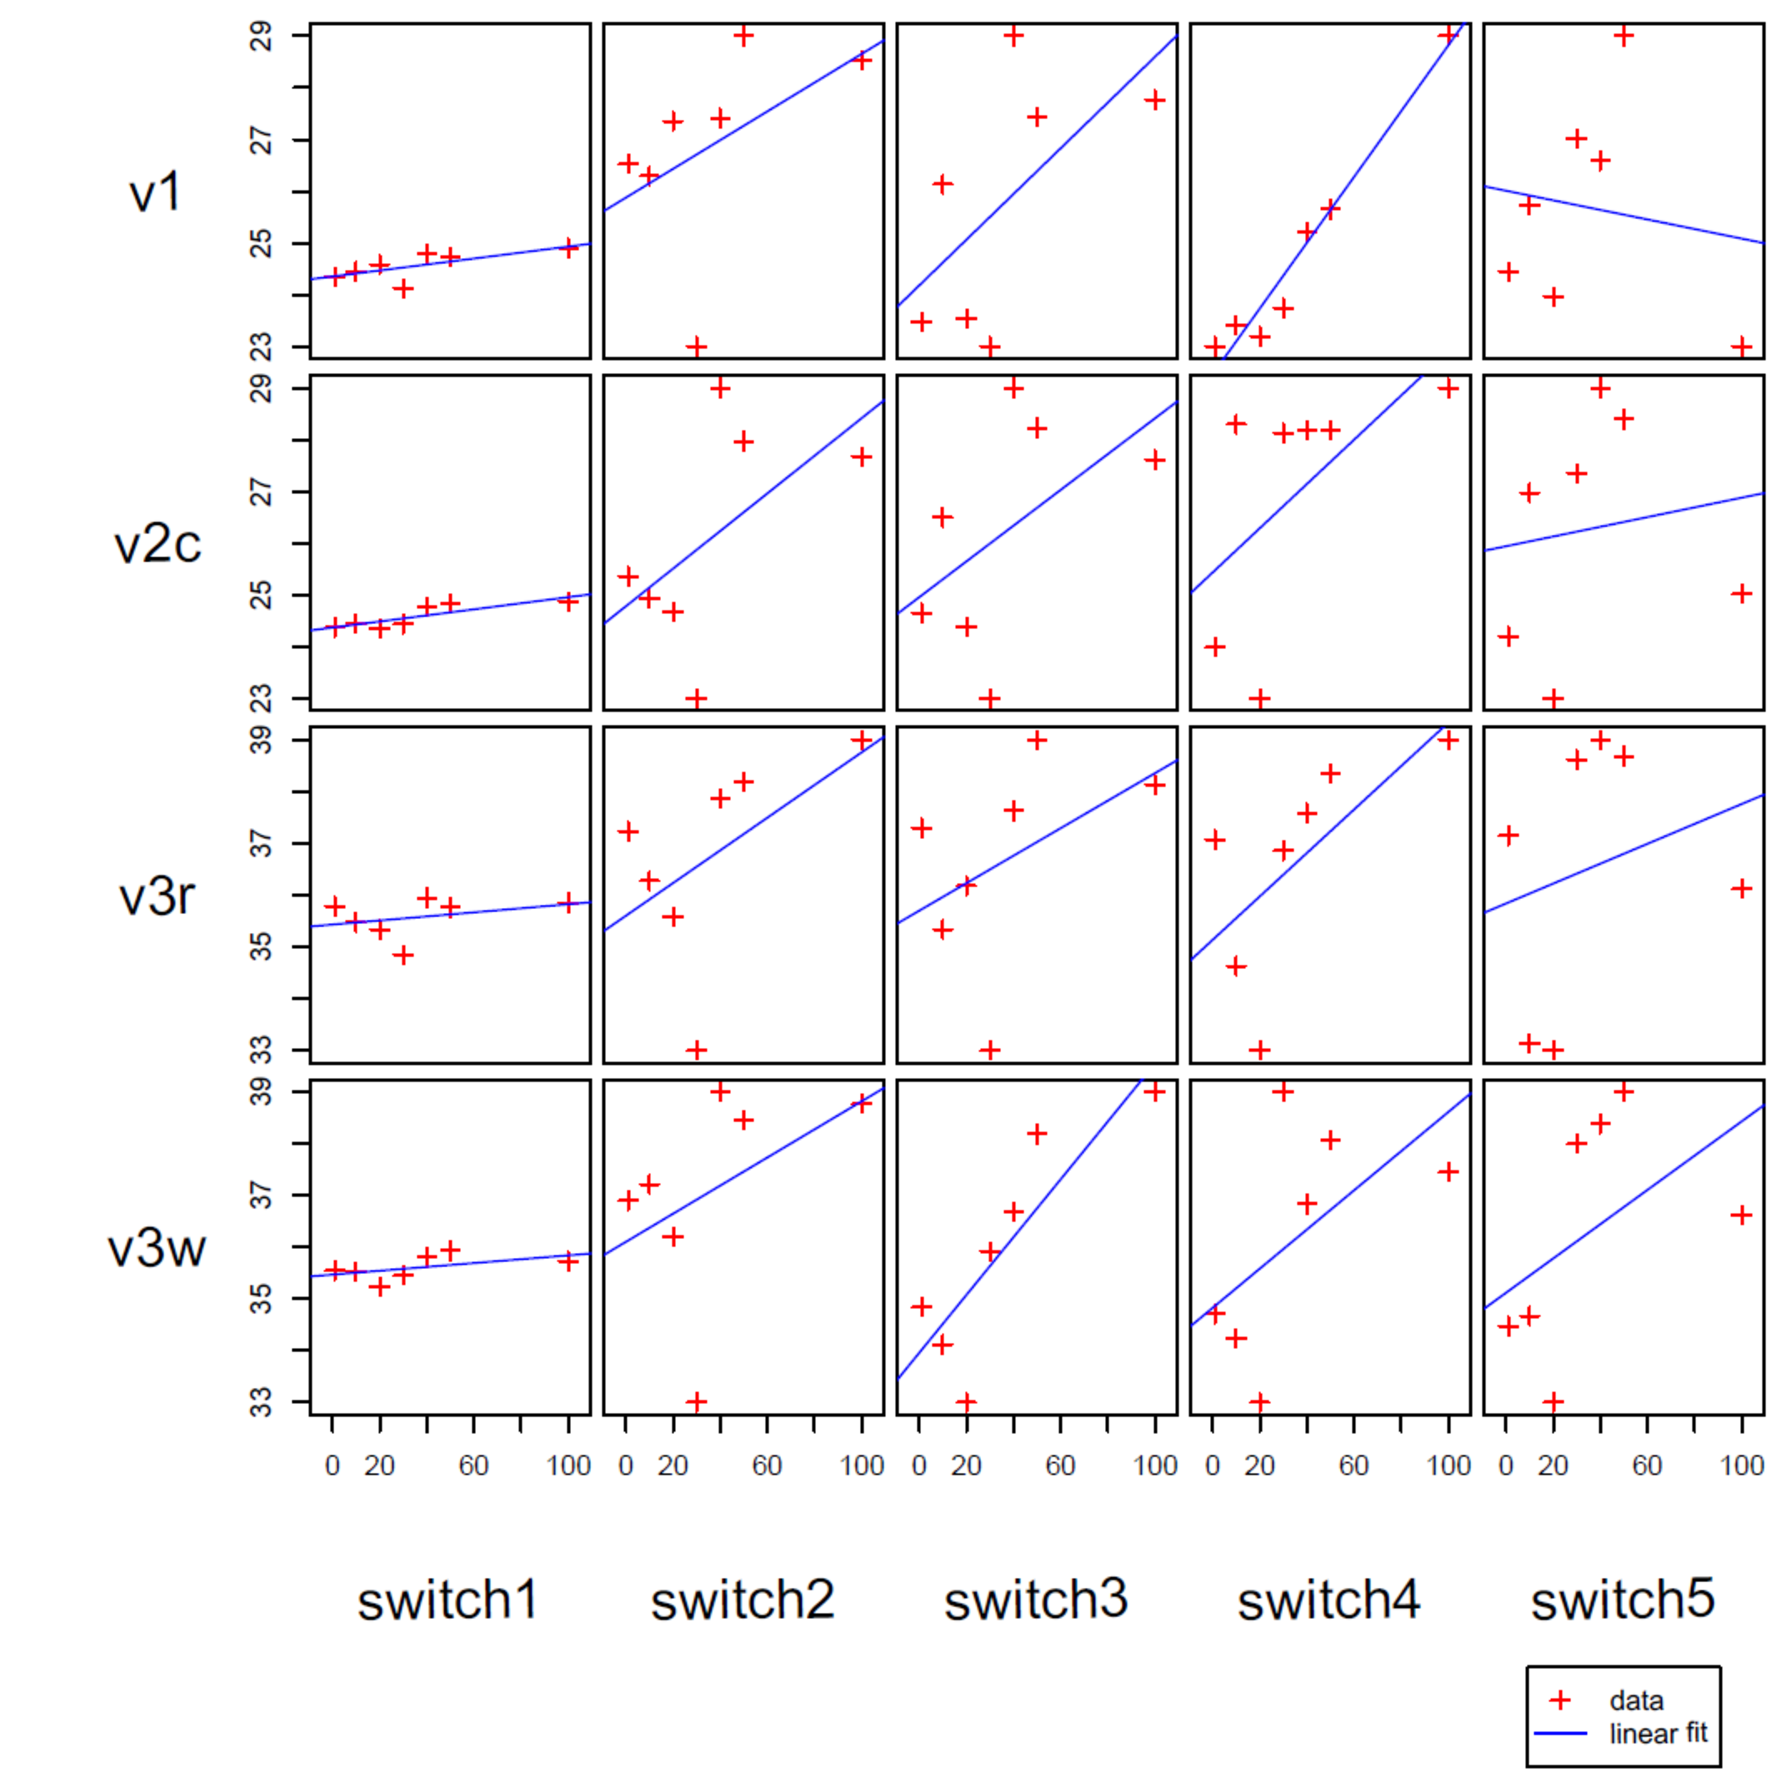
\includegraphics[width=0.88\textwidth]{./images/7point_sleep1s.eps}
  \caption{7-point 산점도와 linear그래프 (Sleep 1s)}
  \label{fig:7ps1}   
\end{figure}

\clearpage

\subsubsection{3.3.2.2 다중회귀분석}
 케이블 길이를 독립변수로 응답시간과의 관계를 회귀분석한 후 케이블 길이, 스위치 개수와 응답시간의 관계 확인을 위해 다중회귀분석을 수행하였다. 여기서 독립변수는 케이블 길이(l)와 스위치 개수(s)이며, 종속변수는 응답시간(t)이다. 이를 나타내는 방정식은 회귀모델이며, 실험의 회귀모델은 식 \ref{eq:eps3}과 같다. 
 
 \begin{equation} \label{eq:eps3}
   t=\alpha_1 l + \alpha_2 s +\beta  
 \end{equation}
 
 다중회귀분석을 통해 얻은 회귀식은 식 \ref{eq:eps4}와 같으며, 그림 \ref{fig:multilinear_v3w}은 다중회귀분석 그래프이다. 다른 버전에서의 결과는 APPENDIX A를 참조 바란다. 
 
 \begin{equation} \label{eq:eps4}
   t=4.416e^-06\alpha_1 - 4.214e^-06\alpha_2 + 3.546e^-02 
 \end{equation}
 
 \begin{figure}[!h]
   \centering
   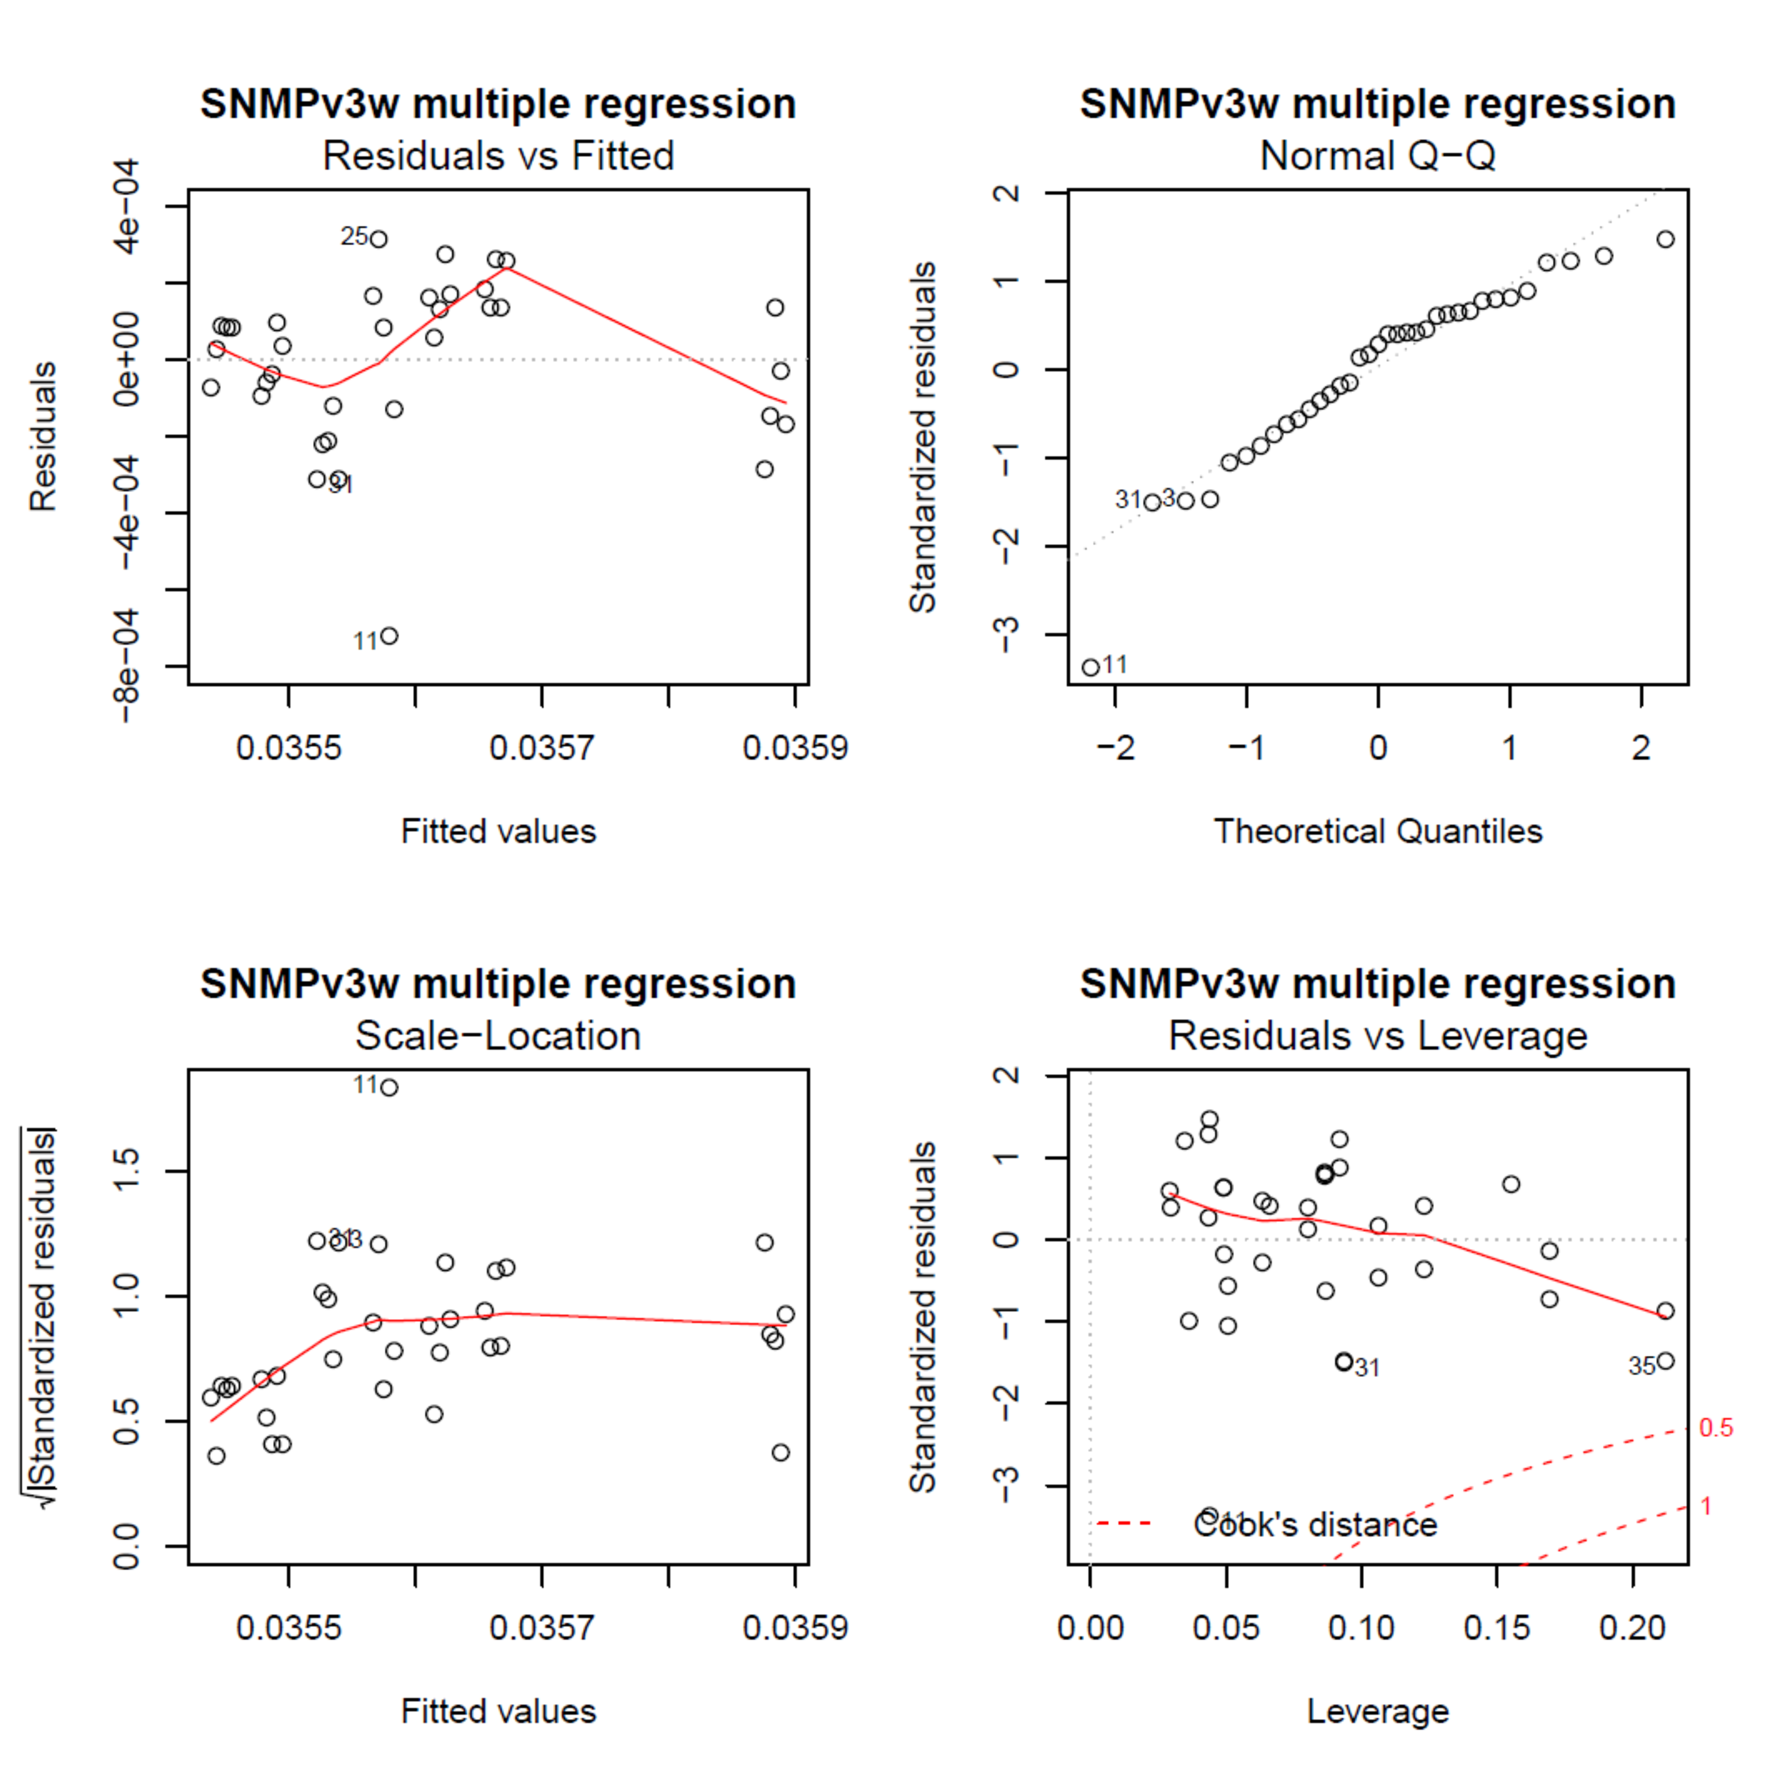
\includegraphics[width=0.88\textwidth]{./images/v3w.eps}
   \caption{다중회귀 그래프 (SNMPv3w)}
   \label{fig:multilinear_v3w}   
 \end{figure}
 
 
 
 \subsection{3.4.3 회귀분석 결과와 가설 검증}
\subsubsection{3.4.3.1 단순회귀분석}
단순회귀분석은 케이블 길이가 길어질수록 응답시간이 커질 것이란 가설의 타당성 입증을 위해 수행되었다. 표 \ref{table:regression}는 그림 \ref{fig:s3s1}에서 v3w의 회귀분석 결과이다. 
 
\begin{table}[!htb]
\begin{center}
\begin{tabular}{c|c}\hline
Independent variable & Value  \\ \hline\hline
p-value &  0.0155\\ 
F-value &  13\\ 
$  R^2  $ &  0.722\\ 
$ Adjusted R^2 $ & 0.666 \\ \hline
\multicolumn{2}{l}{*p < 0.05} \\ \hline\hline
\end{tabular}
\caption{v3w의 단순회귀분석 결과}
  \label{table:regression}  
\end{center}
\end{table} 

회귀분석에서 $  R^2  $은 종속변수(a)의 총 변동에서 독립변수(b)의 변동으로 설명되는 부분이 차지하는 비중을 의미한다. 스위치가 3개 연결되었을 때, v3w의 경우 응답시간 변동의 약 72.2 \%를 케이블 길이 변동으로 설명할 수 있다. 또한, p-value가 0.0155로 α인 0.05보다 작으므로 앞서 세운 가설이 통계적으로 유의하다고 할 수 있다. 다른 조건에서의 결과는 APPENDIX A를 참고하기 바란다.

\subsubsection{3.4.3.2 다중회귀분석}
다중회귀분석은 케이블 길이가 길어질수록 스위치의 개수가 증가할수록 응답시간이 커질 것이란 가설의 타당성 입증을 위해 수행되었으며, v3w에서의 결과는 표 \ref{table:multiregression}과 같다. 

\begin{table}[!htb]
\begin{center}
\begin{tabular}{c|c}\hline
Independent variable & Value  \\ \hline\hline
p-value &  0.003894\\ 
F-value &  6.632\\ 
$  R^2  $ &  0.293\\ 
$ Adjusted R^2 $ & 0.2488 \\ \hline
\multicolumn{2}{l}{*p < 0.05} \\ \hline\hline
\end{tabular}
\caption{v3w의 단순회귀분석 결과}
  \label{table:multiregression}  
\end{center}
\end{table} 

단순회귀분석과 마찬가지로 p-value가 0.003894로 α인 0.05보다 작으므로 앞서 세운 가설이 통계적으로 유의하다고 할 수 있다. 그러나 Adjusted $  R^2  $값이 0.2488로 SNMP 응답시간은 케이블 길이와 스위치 개수 두 변수에 의해 약 24\%가 설명된다.

 \subsection{3.4.4 문제점 및 해결방안}
여러 가지 실험 환경에서 특정 케이블 길이에서 예측된 응답시간과 실제 측정된 응답시간은 오차범위 내에 속했지만, 스위치 개수와 케이블 길이와 응답시간의 변수 간 회귀관계를 설명하기는 어렵다. 이는 분석에 사용된 샘플링의 수의 부족, 사용된 케이블 길이 간 오차, 하드웨어 자체의 속도 등의 테스트 환경이 완벽하게 같지 않아 정밀한 실험이 불가능했다는 점을 이유로 꼽을 수 있다.  따라서 샘플링의 수를 증가시키고 실험 환경을 보완한 후, APC사의 PDU와 현재 SNMP 세 가지 버전을 지원하는 다른 장비를 사용하여 추가적인 응답시간 실험이 필요할 것으로 보인다. 이는 EPICS 통합을 완료 후 좀 더 세밀한 조건들 하에서 진행될 예정이다.

\clearpage
\appendix
\addappheadtotoc
\renewcommand*\printchaptername{\Large\bfseries\appendixname~}
\chapter{SNMP 버전별 응답시간 실험}

본 장은 앞서 수행한 SNMP 버전별 응답시간 테스트를 위한 Bash Script와 R로 수행한 단순회귀분석 및 다중회귀분석의 결과를 보여준다.

\section{응답시간 실험 Bash Script}
SNMP 버전별 응답시간 테스트에 사용된 Bash Shell Script의 CLI를 통해 Listing \ref{list:lst1}과 같이 동작한다. 이 Script를 통해 응답시간 측정 및 데이터 테이블 생성과 R을 이용한 linear 그래프와 히스토그램 그래프를 그릴 수 있다.

\begin{lstlisting}[style=termstyle, caption=SNMP 응답시간 테스트 Script CLI, label={list:lst1}]]
mijoy0909@mjpark:~/users/mijoy0909$ ./speedtest.sh

**********************************
*               OPTIONS          *
**********************************
  [1] SNMP Speed Test             
  [2] File Merge                  
  [3] R(Linear)                   
  [4] R(Histogram)                
----------------------------------
----------------------------------
  [5] Edit R(linear)              
  [6] Edit R(histogram)           
----------------------------------
----------------------------------
  [q] Exit                        
  [0] Help                        
**********************************
-> Select sub option: 1

****************************************
*              SUB OPTIONS             *
****************************************
  [1] SNMP v1        / sleep x          
  [2] SNMP v1        / sleep 1          
  [3] SNMP v2c       / sleep x          
  [4] SNMP v2c       / sleep 1          
  [5] SNMP v3(read)  / sleep x          
  [6] SNMP v3(read)  / sleep 1          
  [7] SNMP v3(write) / sleep x          
  [8] SNMP v3(write) / sleep 1          
  [b] Back                              
  [q] Exit                              
  [0] Help                              
***************************************
-> Select sub option: 1

Enter name you wish to save [ex.S3V3RSXC100] :S2V1SXC50
/home/mijoy0909/speedtest
outletOn
outletOn
outletOn
{...}
-----------------------------------------------
<real>

Total count        :       1000
Mean               : 0.10005000
Sample Deviation   : 0.00899880
Standard Deviation : 0.00899430

-----------------------------------------------
<user>

Total count        :       1000
Mean               : 0.06449000
Sample Deviation   : 0.00647934
Standard Deviation : 0.00647610

-----------------------------------------------
<sys>

Total count        :       1000
Mean               : 0.00358000
Sample Deviation   : 0.00515851
Standard Deviation : 0.00515593

***********************************************

Mean(user+sys)             : 0.03403500
Sample Deviation(user+sys) : 0.00828203

***********************************************
-----------------------------------------------
\end{lstlisting}

\clearpage
\section{응답시간 실험 결과}
본 절은 앞서 설명했던 다양한 환경에서의 응답시간에 대한 회귀분석 결과와 그래프를 보여준다. 그래프의 범례 및 회귀분석에 대한 정보는 3장을 참고 바란다.

\subsection{A.2.1 스위치 개수, 케이블 길이와 응답시간의 관계}


본 절에서는 표 \ref{table:sx}의 Sleep을 하지 않은 환경에서 1,000번 측정한 응답시간의 평균값을 이용하여 스위치 개수, 케이블 길이와 응답시간의 관계를 확인한다.

\begin{table}[!htb]
\begin{center}
\begin{tabular}{c|c|c|c|c|c|c}\hline
 & Version & Switch1 & Switch2 & Switch3 & Switch4 & Switch5\\ \hline
1m & v1 & 25.97 & 26.26 & 26.27 & 26.40& 26.17 \\ 
& v2c & 26.11 & 26.10 & 26.20 & 25.98 & 26.01 \\ 
& v3r & 35.70 & 35.83 & 35.71 & 35.77 & 35.65 \\ 
& v3w & 35.74 & 35.62 & 35.77 & 35.61 & 35.50 \\\hline
50m & v1 & 26.20 & 26.56 & 26.25 & 26.39 & 26.22 \\ 
& v2c & 26.41 & 26.35 & 26.33 & 26.12 & 26.30 \\ 
& v3r & 36.28 & 36.22 & 36.09 & 36.12 & 36.10 \\ 
& v3w & 36.06 & 36.16 & 36.17 & 36.02 & 36.39\\\hline
100m & v1 & 26.54 & 26.72 & 26.43 & 26.41 & 26.20 \\
& v2c & 26.41 & 26.20 & 26.13 & 26.25 & 26.29 \\
& v3r & 36.26 & 36.04 & 36.16 & 35.85 & 36.03 \\
& v3w & 35.99 & 36.02 & 35.99 & 35.80 & 35.91 \\\hline \hline
\end{tabular}
\caption{SNMP 버전별 응답시간의 평균값 (non-sleep) (단위 : ms)}
  \label{table:sx}  
\end{center}
\end{table} 

변수들의 상관관계를 확인한 결과 그림 \ref{fig:3psx}, \ref{fig:7psx}와 같이 스위치 개수 증가에 따른 응답시간의 변화는 적지만, 케이블 길이 변화에 대한 응답시간은 대부분 증가함을 알 수 있다.

\begin{figure}[!htb]
  \centering
  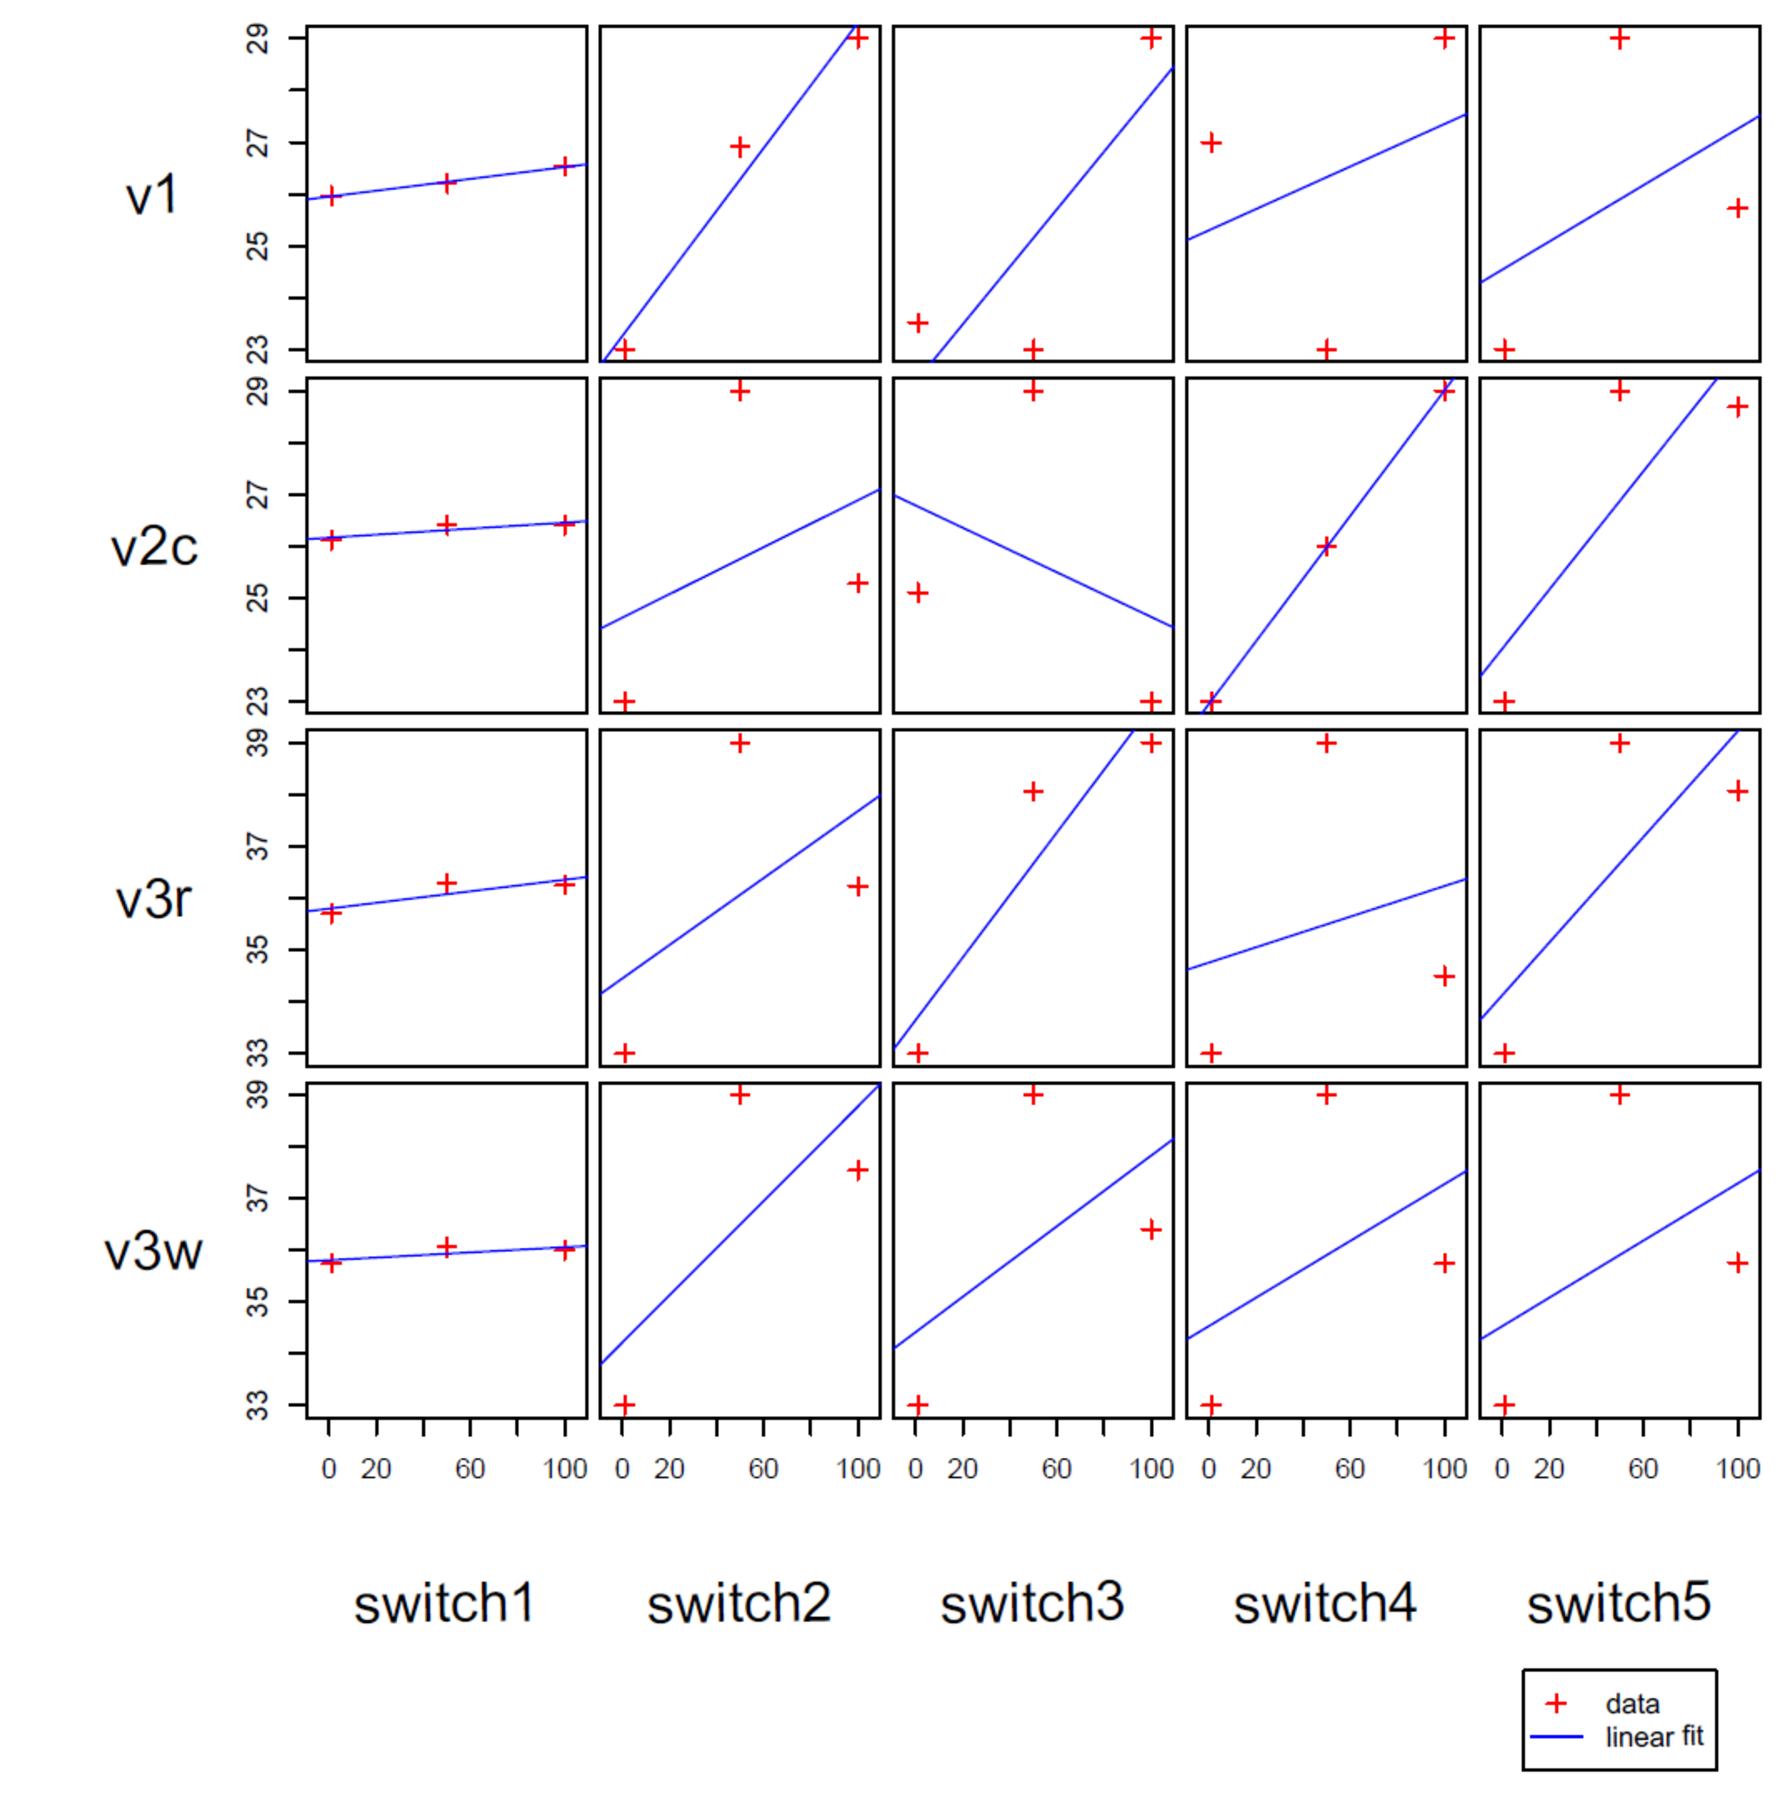
\includegraphics[width=0.9\textwidth]{./images/3point_sleepx.eps}
  \caption{3-point 산점도와 linear그래프 (Sleep 1x)}
  \label{fig:3psx}   
\end{figure}

\begin{figure}[!htb]
  \centering
  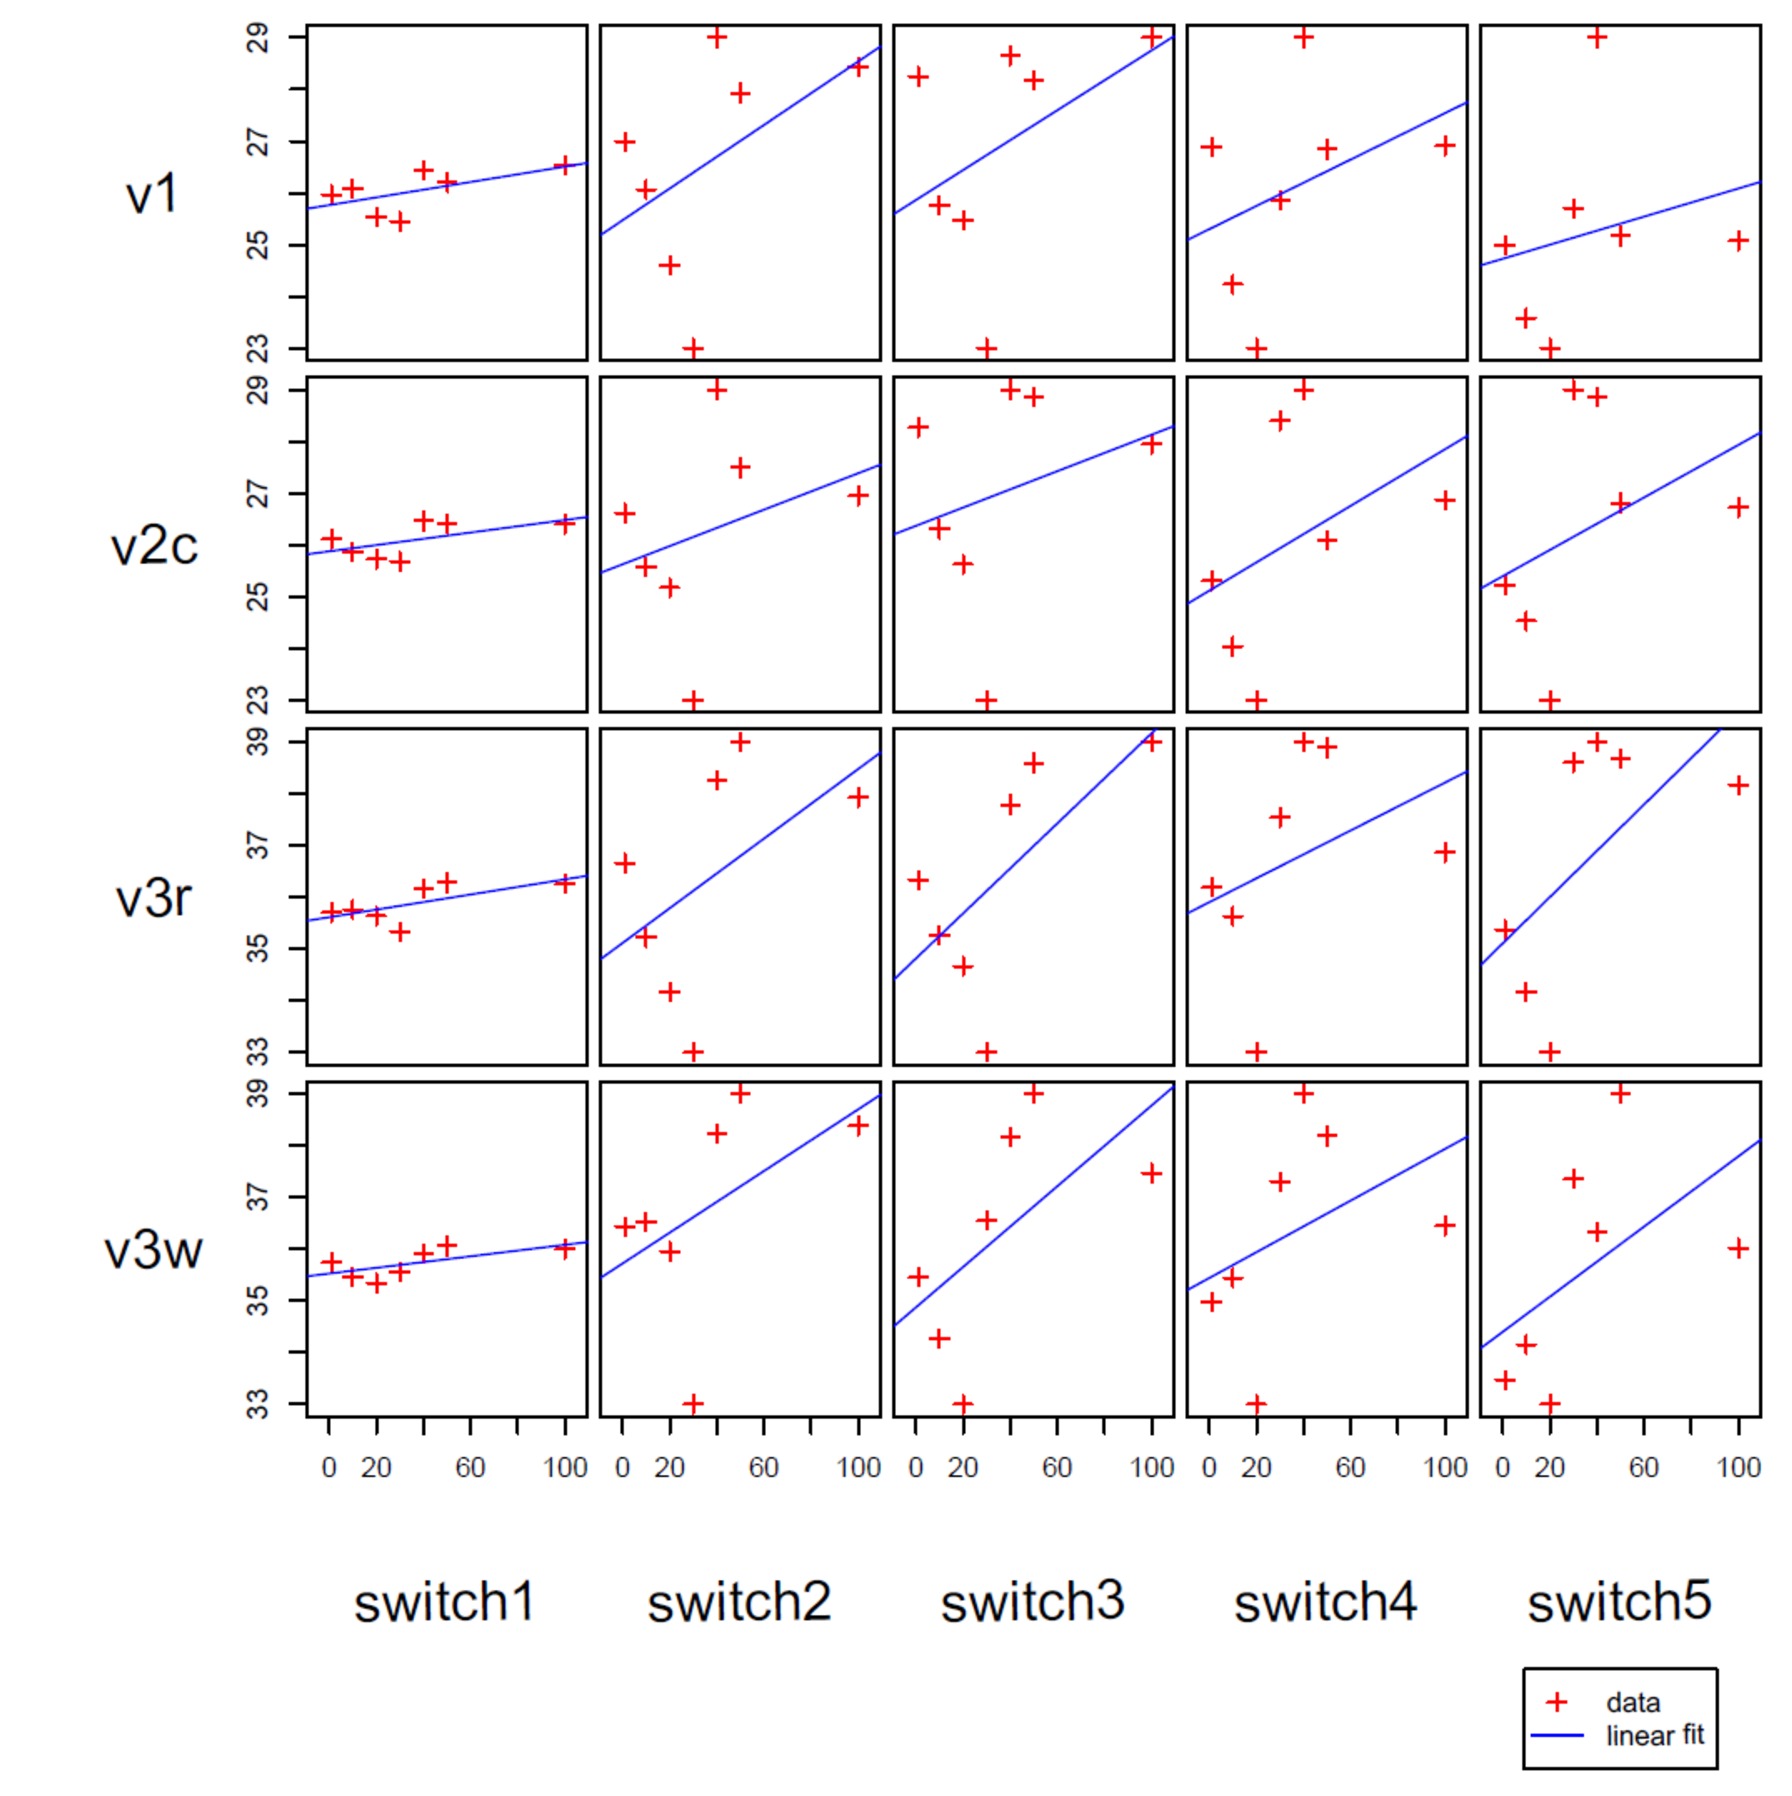
\includegraphics[width=0.9\textwidth]{./images/7point_sleepx.eps}
  \caption{7-point 산점도와 linear그래프 (Sleep 1x)}
  \label{fig:7psx}   
\end{figure}

\clearpage
\subsection{A.2.2 단순회귀분석 그래프와 결과}
\subsubsection{A.2.2.1 Switch 1}
\paragraph{1) Non-Sleep}
    
\begin{figure}[h!]
  \centering
  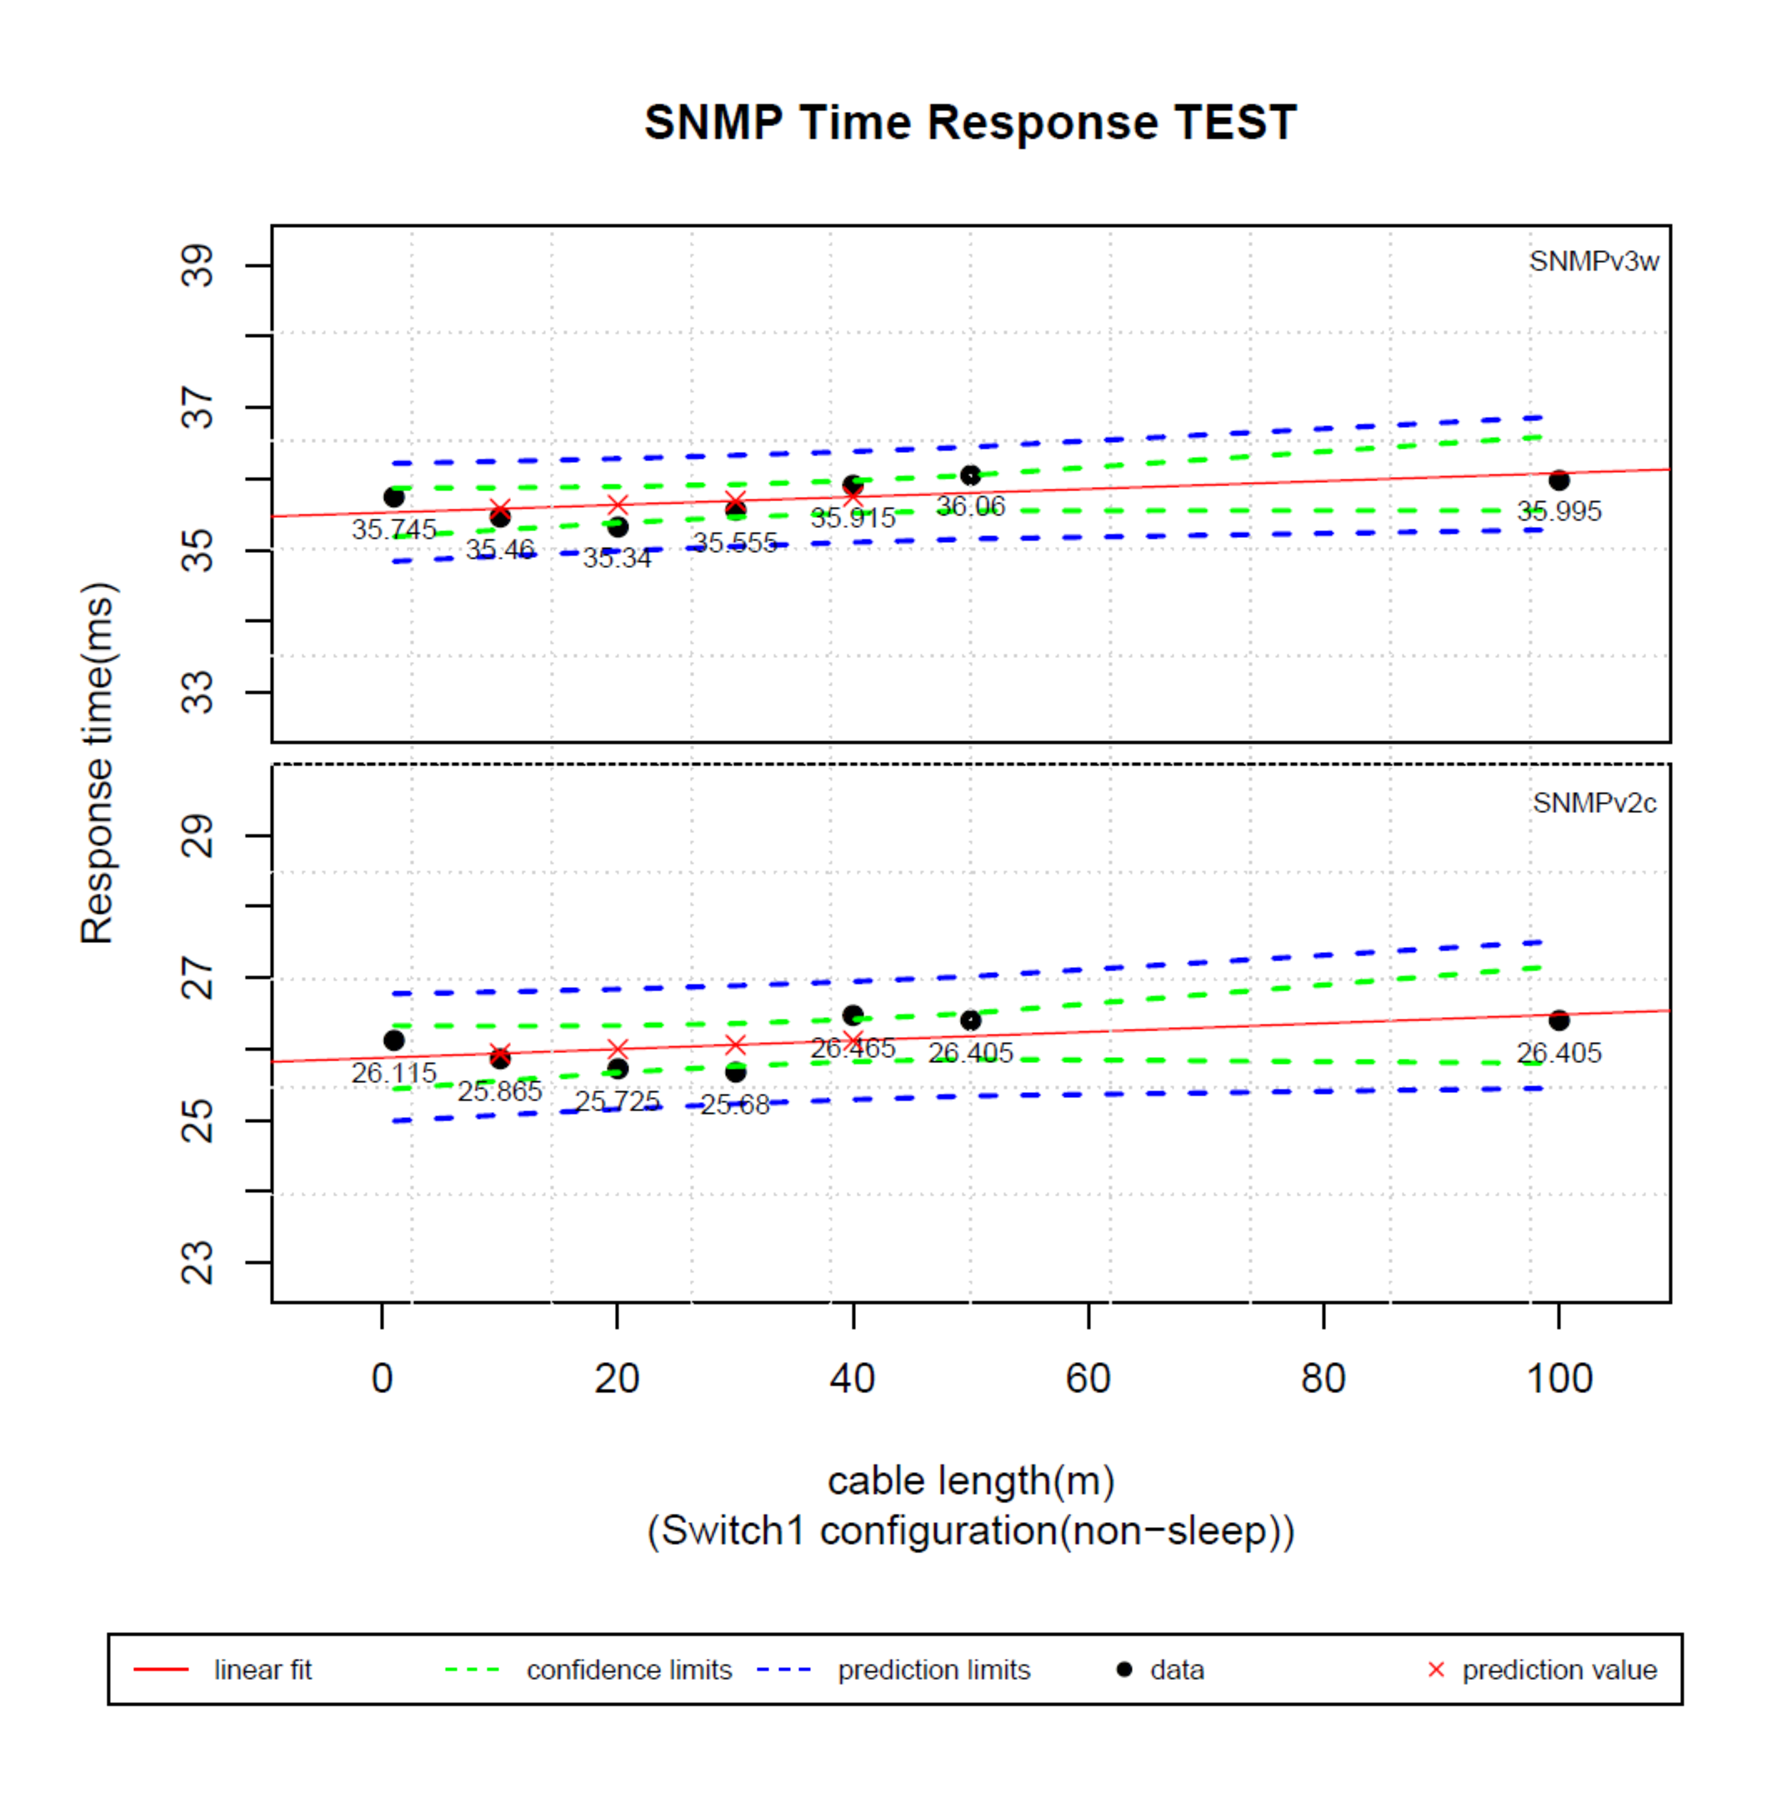
\includegraphics[width=0.5\textwidth]{./images/s1sx.eps}
  \caption{Switch1/Non-Sleep 회귀분석 그래프}
\end{figure}


\begin{table}[!htb]
\begin{center}
\begin{tabular}{c|c|c|c|c}\hline
& \multicolumn{4}{l}{Value} \\ \hline
Independent variable & v1 & v2c & v3r & v3w \\ \hline\hline
p-value& 0.16 & 0.17 & 0.11 & 0.11 \\ \hline
F-value& 2.65 & 2.63 & 3.90 & 3.73 \\ \hline
$  R^2  $ & 0.35 & 0.34 & 0.44 & 0.43 \\\hline
$ Adjusted R^2 $ & 0.02 & 0.21 & 0.33 & 0.31 \\\hline 
\multicolumn{5}{l}{*p < 0.05} \\ \hline
\end{tabular}
\caption{Switch1/Non-Sleep 회귀분석 결과}
\end{center}
\end{table} 


\begin{table}[!htb]
\begin{center}
\begin{tabular}{c|c}\hline
 & 회귀식  \\ \hline\hline
v1 &  $ t=0.007455\alpha + 25.766969 $  \\ 
v2c & $ t=0.005995\alpha + 25.876472 $ \\ 
v3r & $ t=0.007355\alpha + 35.609133 $ \\ 
v3w & $ t=0.005628\alpha + 35.523916 $  \\ \hline
\end{tabular}
\caption{Switch1/Non-Sleep 버전별 회귀식}
\end{center}
\end{table} 


\clearpage
\paragraph{2) Sleep 1s}
    
\begin{figure}[h!]
  \centering
  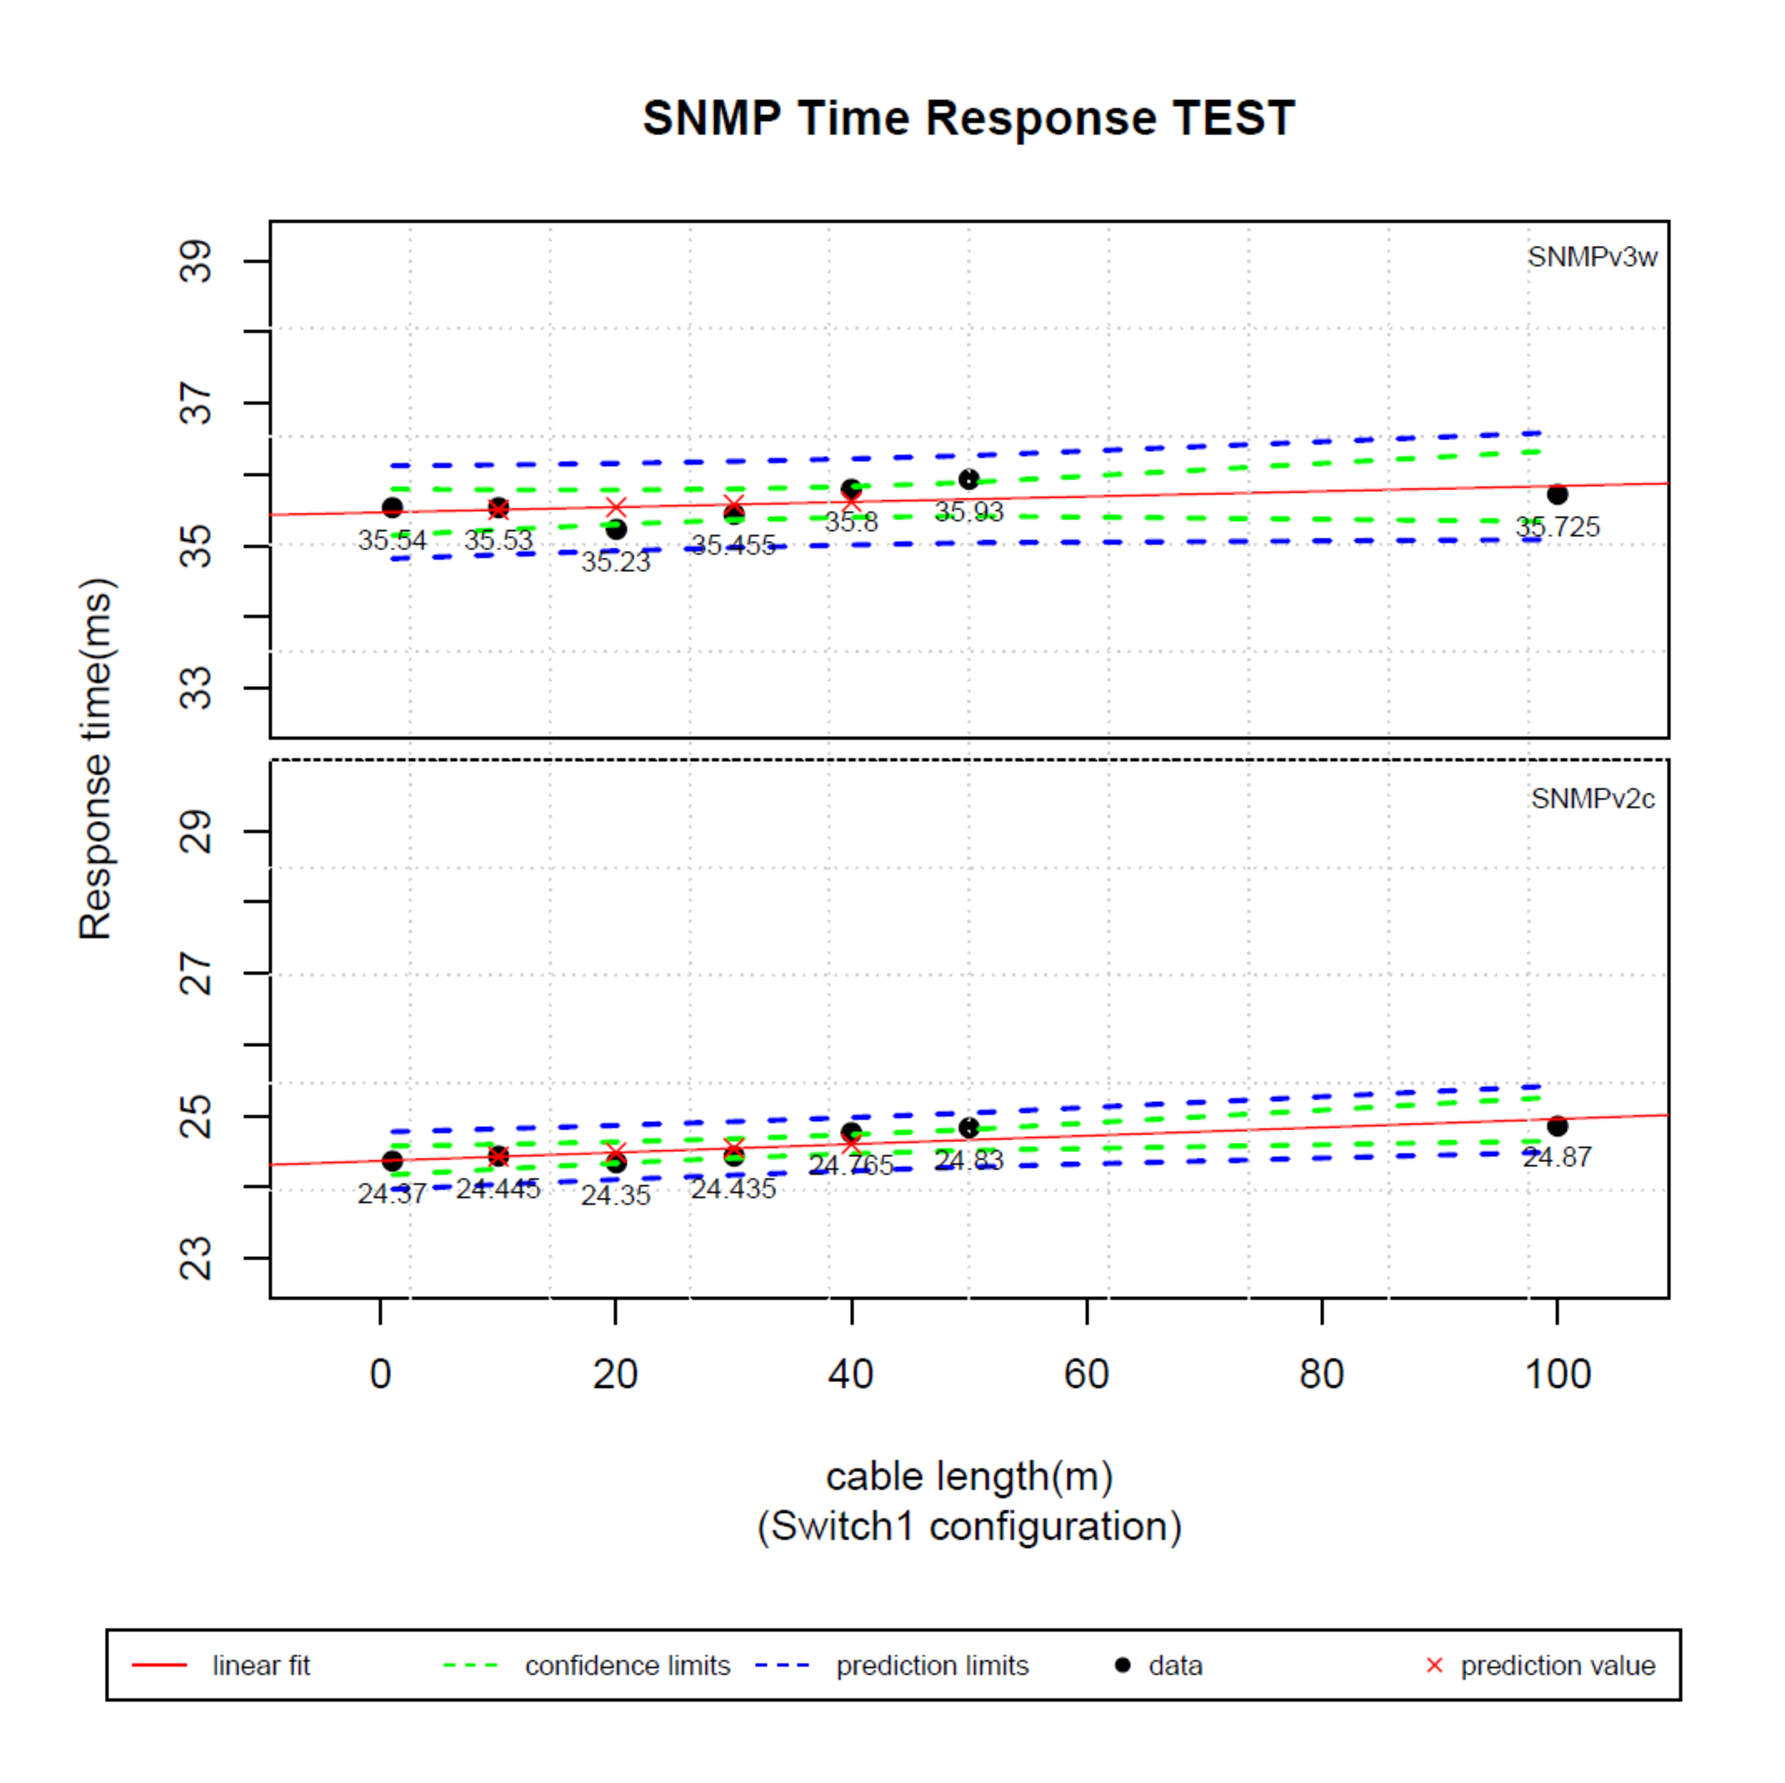
\includegraphics[width=0.5 \textwidth]{./images/s1s1.eps}
  \caption{Switch1/Sleep 1s 회귀분석 그래프}
\end{figure}


\begin{table}[!htb]
\begin{center}
\begin{tabular}{c|c|c|c|c}\hline
& \multicolumn{4}{l}{Value} \\ \hline
Independent variable & v1 & v2c & v3r & v3w \\ \hline\hline
p-value& 0.08 & 0.02 & 0.46 & 0.23 \\ \hline
F-value& 4.79 & 12.10& 0.63 & 1.86 \\ \hline
$  R^2  $ & 0.49 & 0.71 & 0.11 & 0.27 \\\hline
$ Adjusted R^2 $ & 0.39 & 0.65 & -0.07 & 0.13 \\\hline 
\multicolumn{5}{l}{*p < 0.05} \\ \hline
\end{tabular}
\caption{Switch1/Sleep 1s 회귀분석 결과}
\end{center}
\end{table} 


\begin{table}[!htb]
\begin{center}
\begin{tabular}{c|c}\hline
 & 회귀식  \\ \hline\hline
v1 &  $ t=0.005798\alpha + 24.352111 $  \\ 
v2c & $ t=0.005890\alpha + 24.368802 $ \\ 
v3r & $ t=0.003968\alpha + 35.430590 $ \\ 
v3w & $ t=0.003658\alpha + 35.470256 $  \\ \hline
\end{tabular}
\caption{Switch1/Sleep 1s 버전별 회귀식}
\end{center}
\end{table} 



\subsubsection{A.2.2.2 Switch 2}
\paragraph{1) Non-Sleep}
    
\begin{figure}[h!]
  \centering
  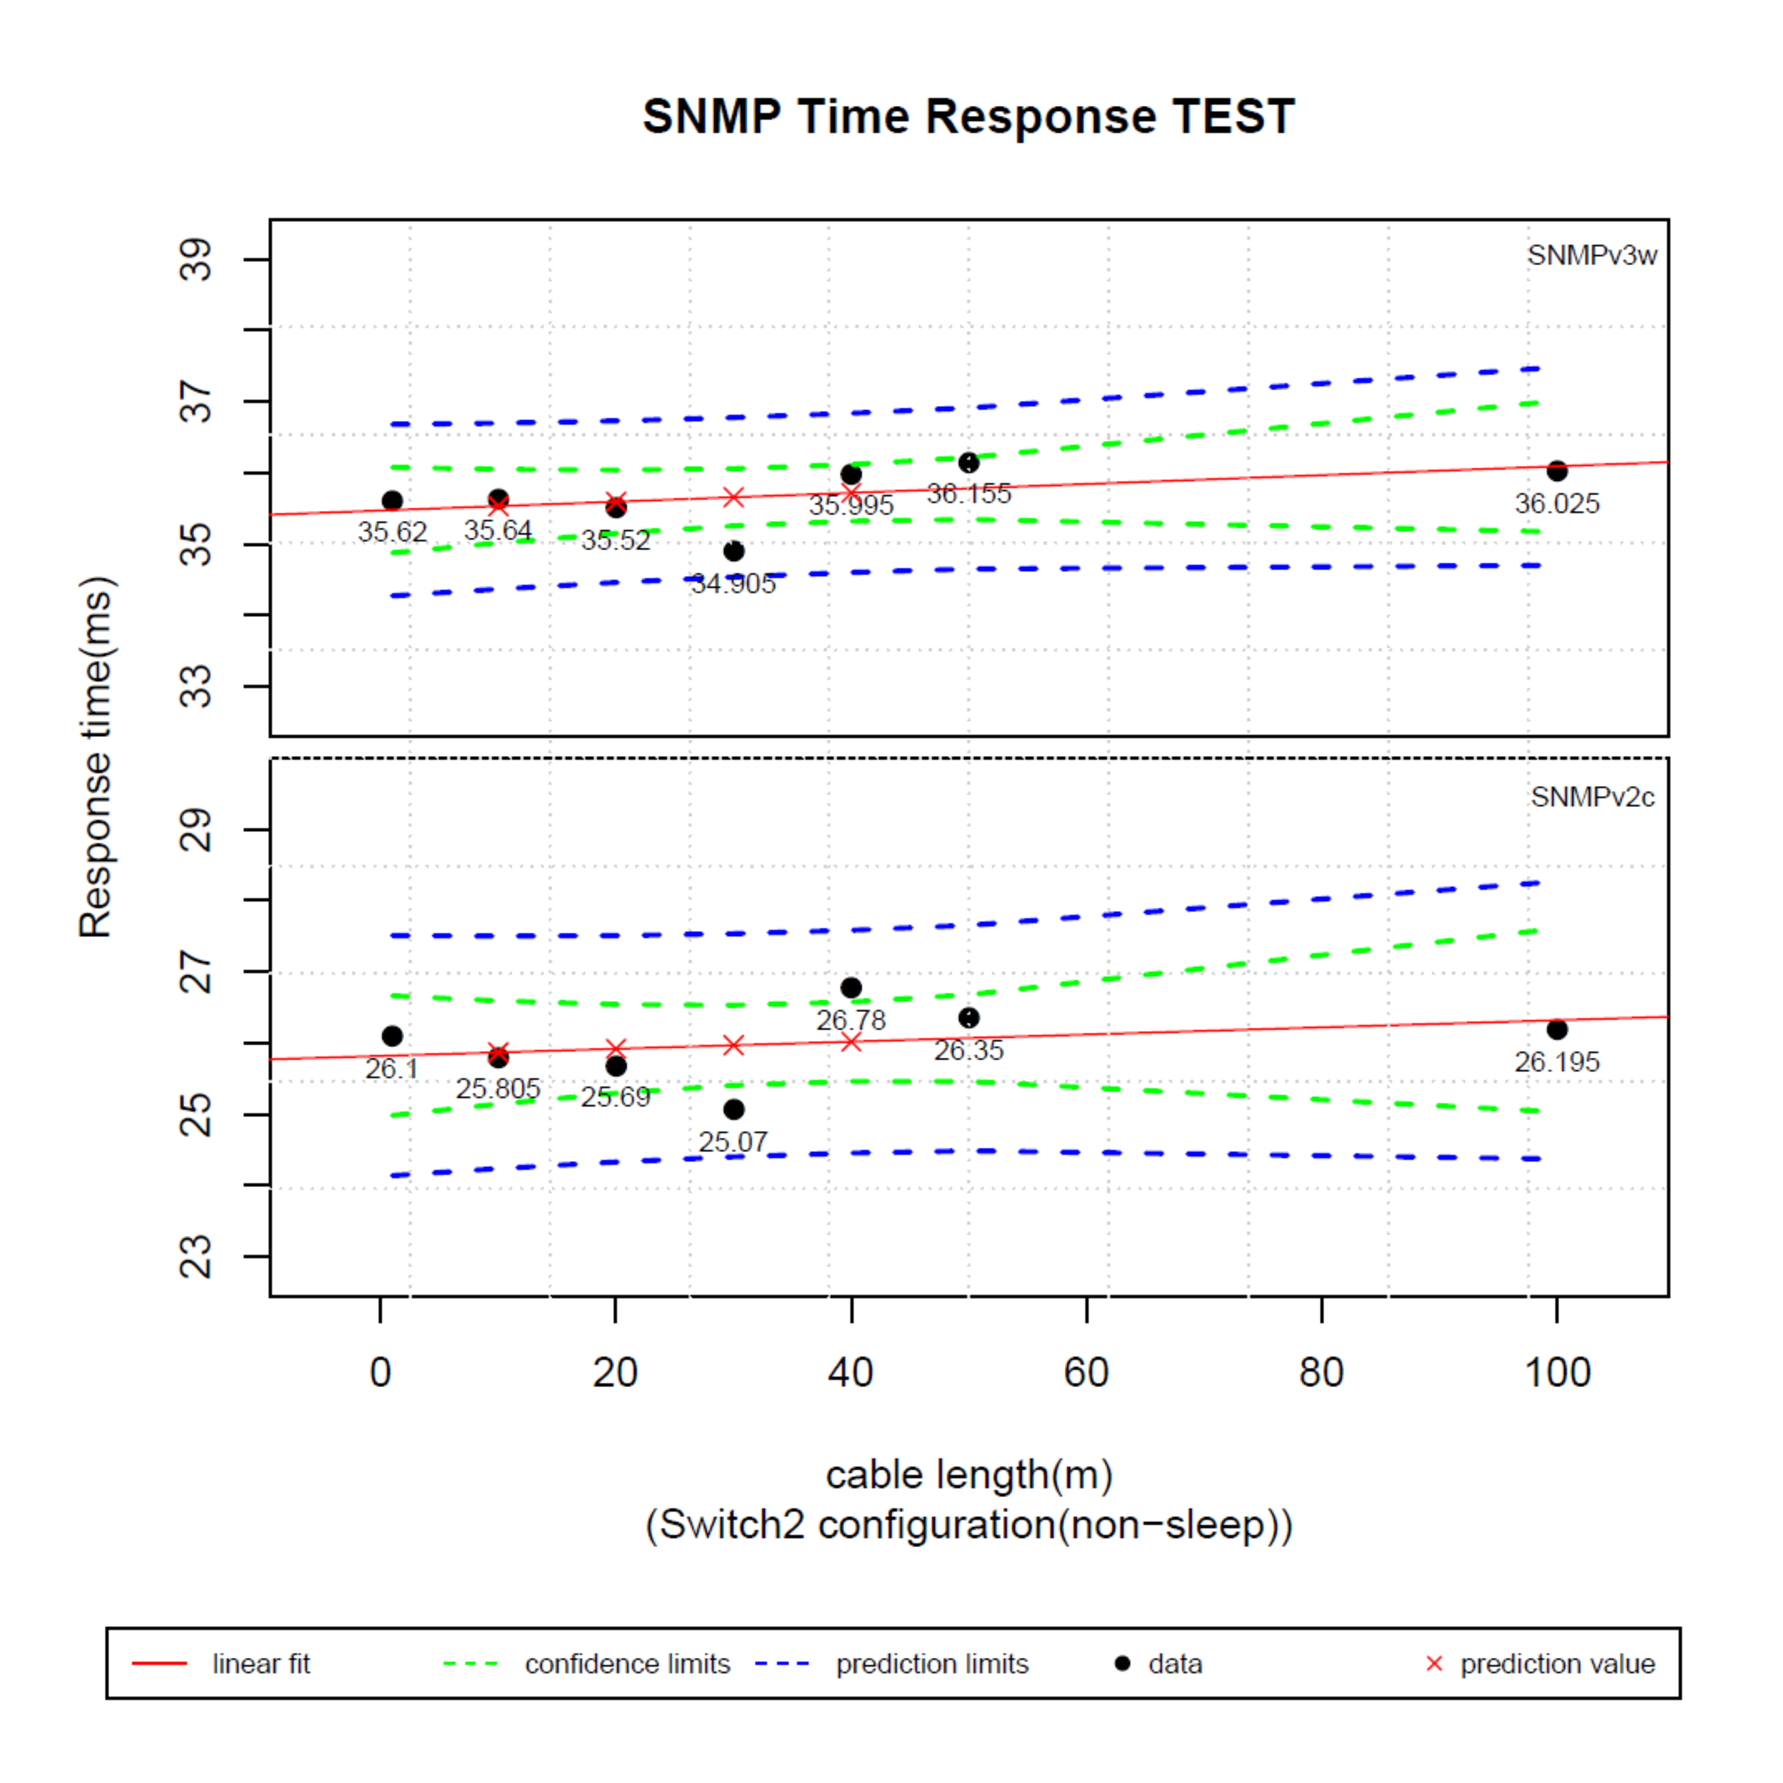
\includegraphics[width=0.5\textwidth]{./images/s2sx.eps}
  \caption{Switch2/Non-Sleep 회귀분석 그래프}
\end{figure}


\begin{table}[!htb]
\begin{center}
\begin{tabular}{c|c|c|c|c}\hline
& \multicolumn{4}{l}{Value} \\ \hline
Independent variable & v1 & v2c & v3r & v3w \\ \hline\hline
p-value& 0.29 & 0.51 & 0.26 & 0.27 \\ \hline
F-value& 1.38 & 0.51 & 1.59 & 1.52 \\ \hline
$  R^2  $ & 0.22 & 0.09 & 0.24 & 0.23 \\\hline
$ Adjusted R^2 $ & 0.06 & -0.09 & 0.09 & 0.08 \\\hline 
\multicolumn{5}{l}{*p < 0.05} \\ \hline
\end{tabular}
\caption{Switch2/Non-Sleep 회귀분석 결과}
\end{center}
\end{table} 


\begin{table}[!htb]
\begin{center}
\begin{tabular}{c|c}\hline
 & 회귀식  \\ \hline\hline
v1 &  $ t=0.009791\alpha + 25.776081 $  \\ 
v2c & $ t=0.005085\alpha + 25.816228 $ \\ 
v3r & $ t=0.005597\alpha + 35.573599 $ \\ 
v3w & $ t=0.006177\alpha + 35.472804 $  \\ \hline
\end{tabular}
\caption{Switch2/Non-Sleep 버전별 회귀식}
\end{center}
\end{table} 


\clearpage
\paragraph{2) Sleep 1s}
    
\begin{figure}[h!]
  \centering
  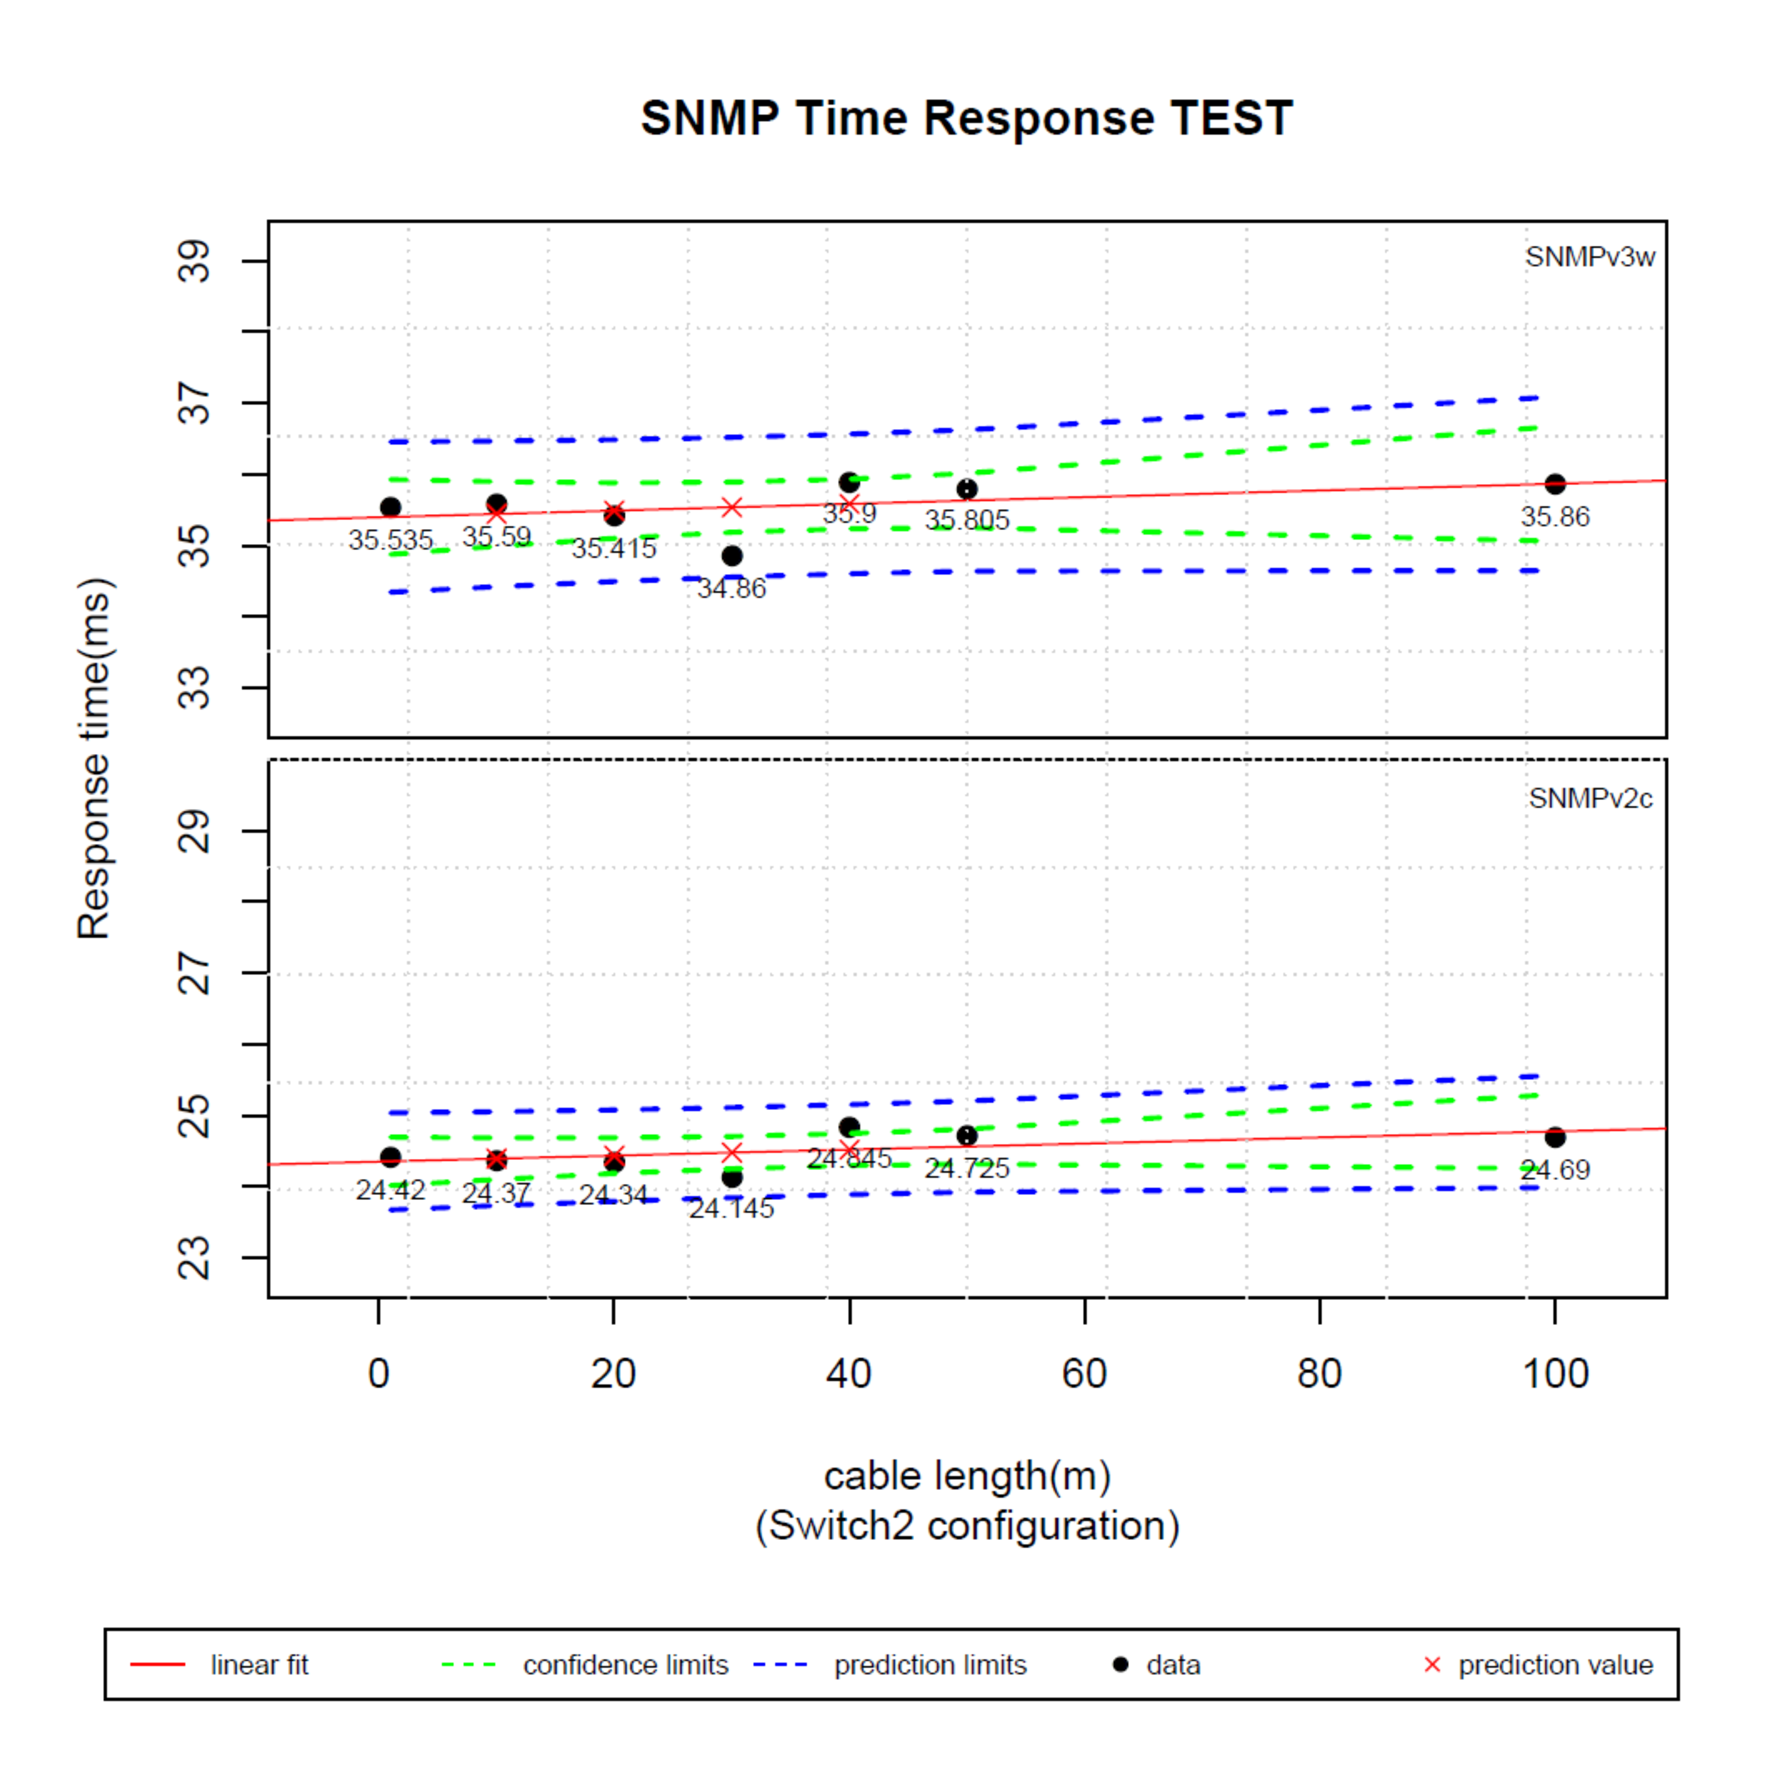
\includegraphics[width=0.5 \textwidth]{./images/s2s1.eps}
  \caption{Switch2/Sleep 1s 회귀분석 그래프}
4\end{figure}


\begin{table}[!htb]
\begin{center}
\begin{tabular}{c|c|c|c|c}\hline
& \multicolumn{4}{l}{Value} \\ \hline
Independent variable & v1 & v2c & v3r & v3w \\ \hline\hline
p-value& 0.29 & 0.18 & 0.24 & 0.34 \\ \hline
F-value& 1.38 & 2.22 & 1.82 & 1.14 \\ \hline
$  R^2  $ & 0.22 & 0.31 & 0.27 & 0.19 \\\hline
$ Adjusted R^2 $ & 0.06 & 0.17 & 0.12 & 0.02 \\\hline 
\multicolumn{5}{l}{*p < 0.05} \\ \hline
\end{tabular}
\caption{Switch2/Sleep 1s 회귀분석 결과}
\end{center}
\end{table} 


\begin{table}[!htb]
\begin{center}
\begin{tabular}{c|c}\hline
 & 회귀식  \\ \hline\hline
v1 &  $ t=0.002358\alpha + 24.394023 $  \\ 
v2c & $ t=0.004231\alpha + 24.351158 $ \\ 
v3r & $ t=0.005422\alpha + 35.274149 $ \\ 
v3w & $ t=0.004713\alpha + 35.396735 $  \\ \hline
\end{tabular}
\caption{Switch2/Sleep 1s 버전별 회귀식}
\end{center}
\end{table} 



\subsubsection{A.2.2.3 Switch 3}
\paragraph{1) Non-Sleep}
    
\begin{figure}[h!]
  \centering
  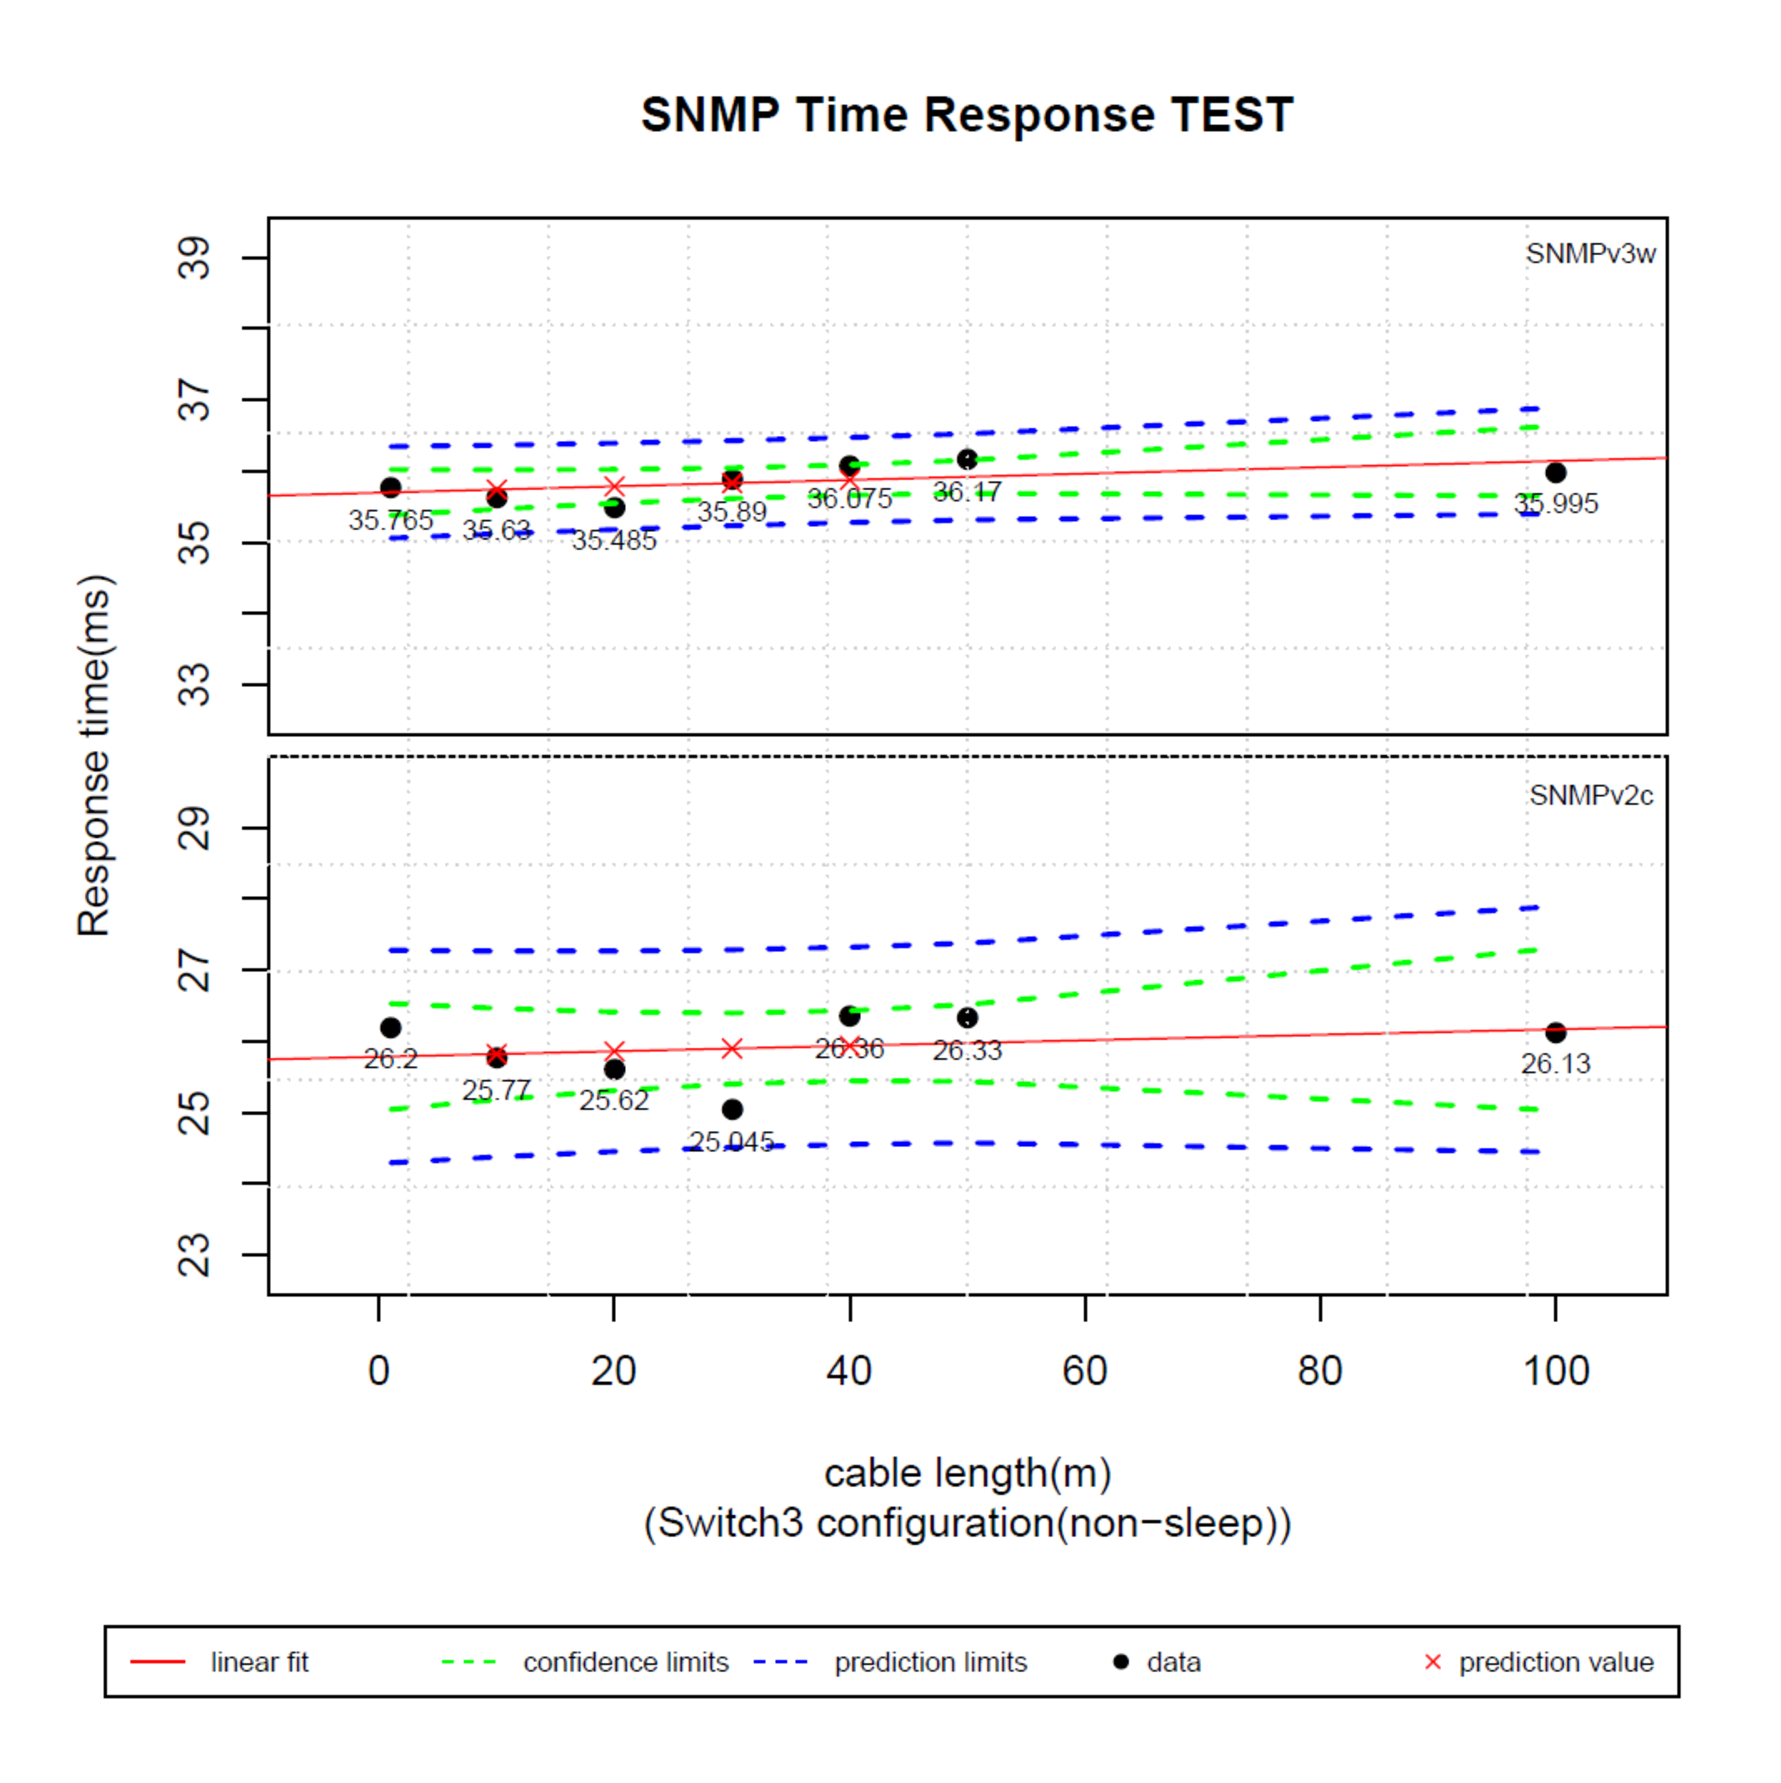
\includegraphics[width=0.5\textwidth]{./images/s3sx.eps}
  \caption{Switch3/Non-Sleep 회귀분석 그래프}
\end{figure}


\begin{table}[!htb]
\begin{center}
\begin{tabular}{c|c|c|c|c}\hline
& \multicolumn{4}{l}{Value} \\ \hline
Independent variable & v1 & v2c & v3r & v3w \\ \hline\hline
p-value& 0.34 & 0.56 & 0.12 & 0.16 \\ \hline
F-value& 1.13 & 0.38 & 3.62 & 2.75 \\ \hline
$  R^2  $ & 0.18 & 0.07 & 0.42 & 0.36 \\\hline
$ Adjusted R^2 $ & 0.02 & -0.12 & 0.30 & 0.23 \\\hline 
\multicolumn{5}{l}{*p < 0.05} \\ \hline
\end{tabular}
\caption{Switch3/Non-Sleep 회귀분석 결과}
\end{center}
\end{table} 

\begin{table}[!htb]
\begin{center}
\begin{tabular}{c|c}\hline
 & 회귀식  \\ \hline\hline
v1 &  $ t=0.006171\alpha + 25.753025 $  \\ 
v2c & $ t=0.003864\alpha + 25.782865 $ \\ 
v3r & $ t=0.007330\alpha + 35.455754 $ \\ 
v3w & $ t=0.004522\alpha + 35.697837 $  \\ \hline
\end{tabular}
\caption{Switch3/Non-Sleep 버전별 회귀식}
\end{center}
\end{table} 


\clearpage
\paragraph{2) Sleep 1s}
    
\begin{figure}[h!]
  \centering
  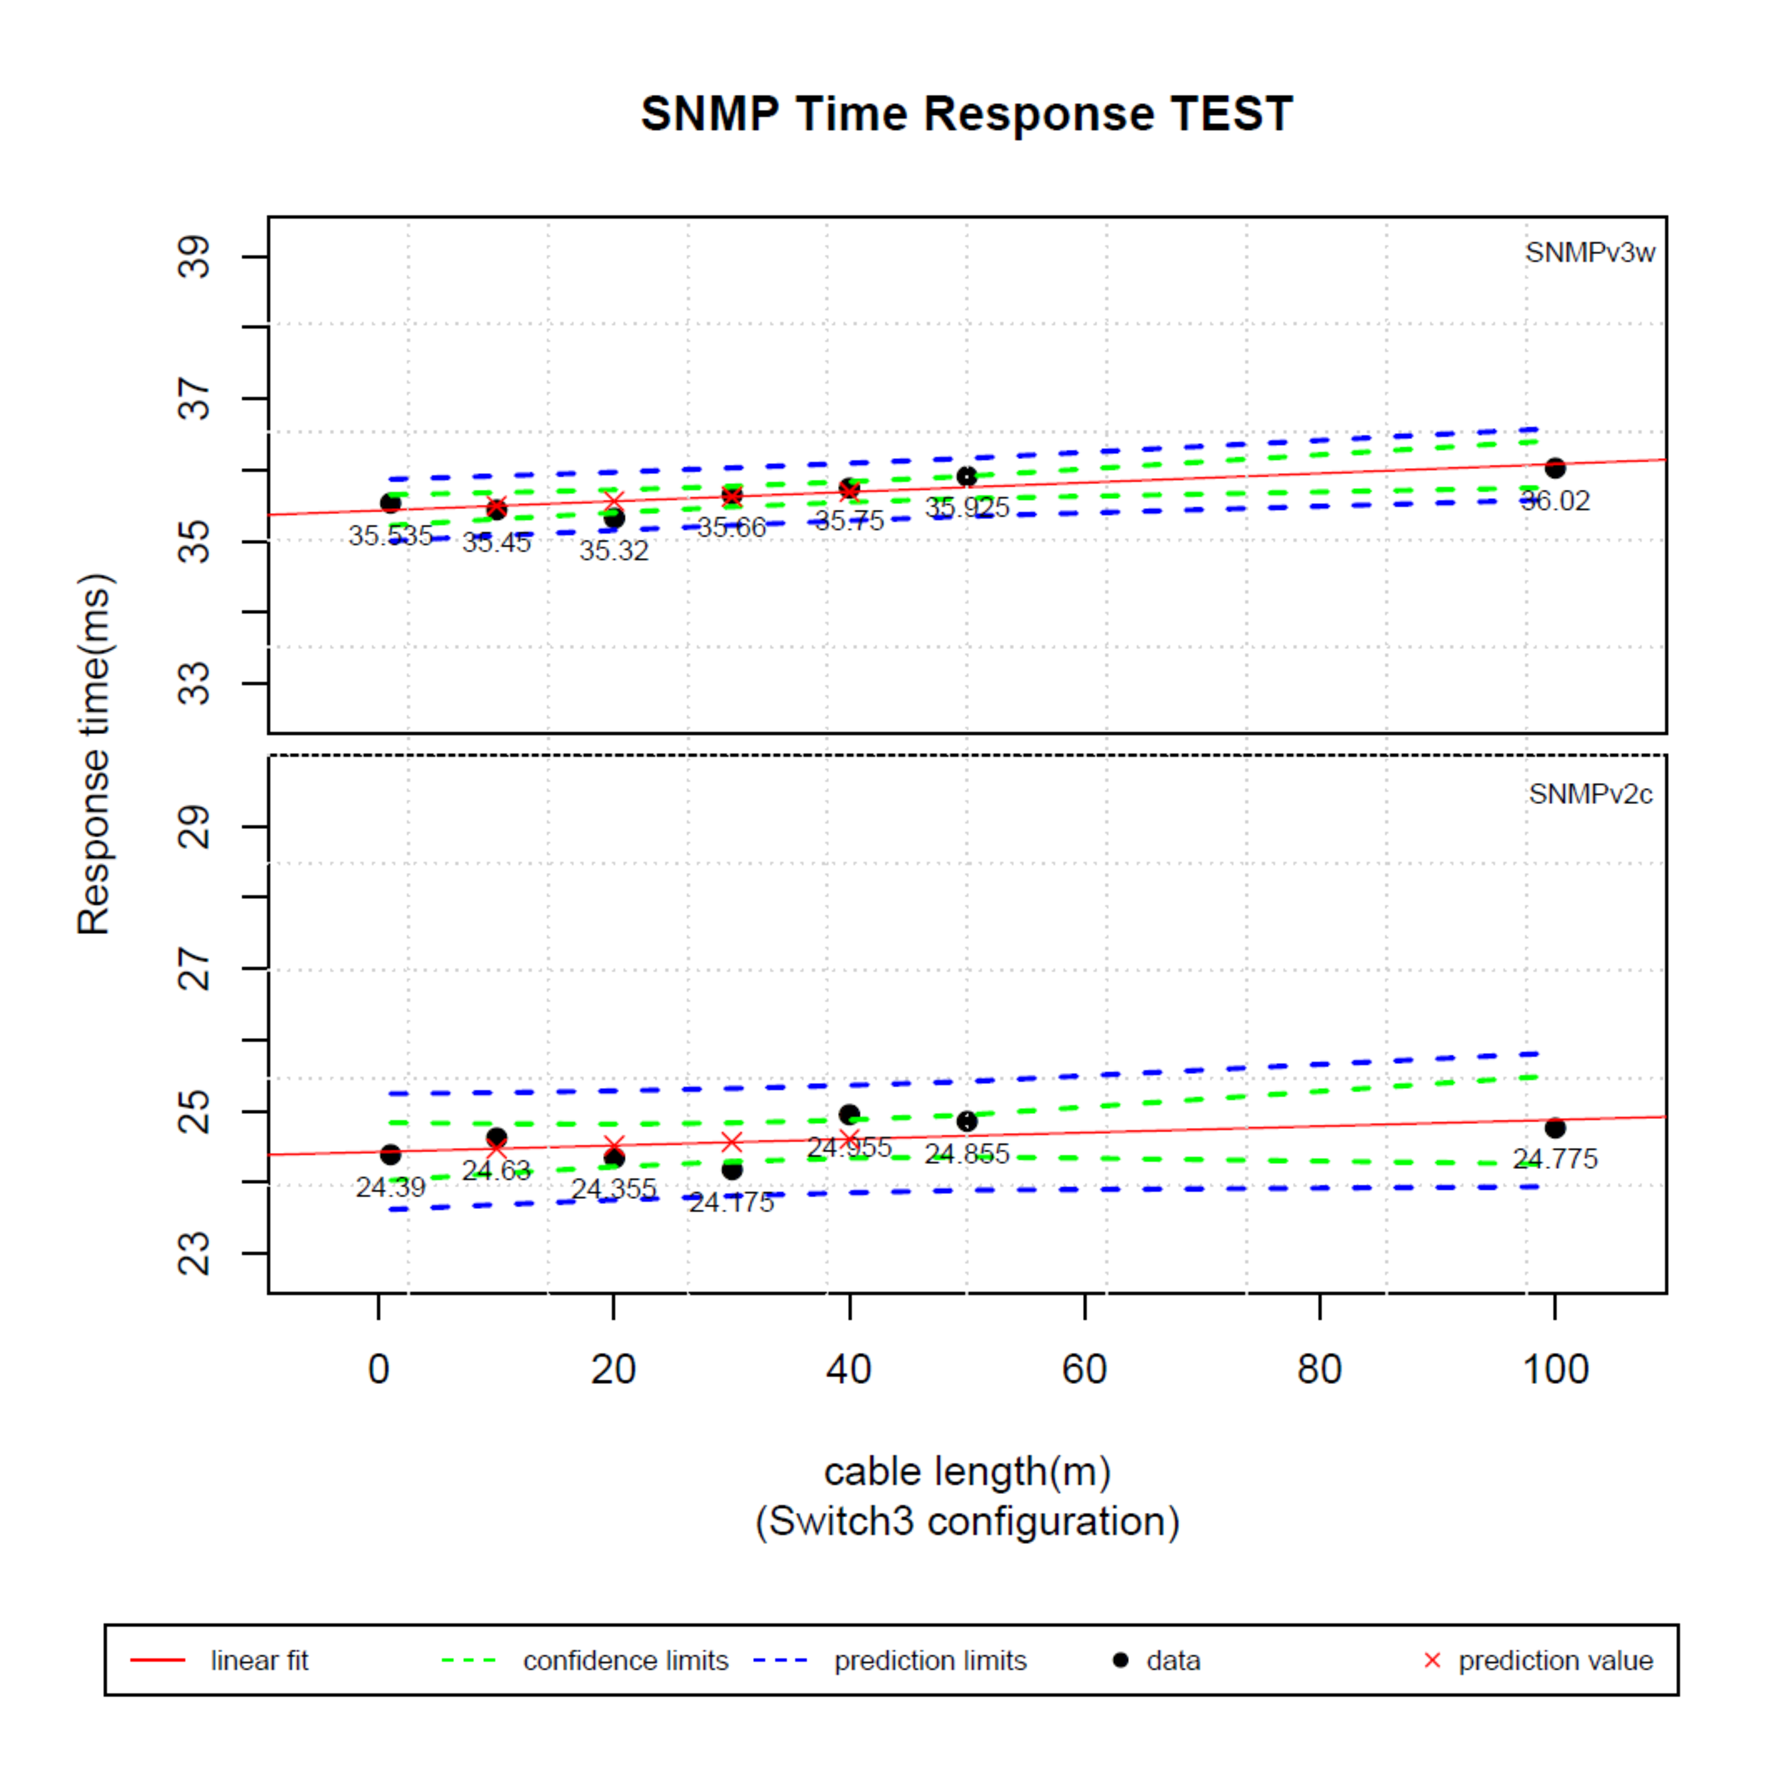
\includegraphics[width=0.5 \textwidth]{./images/s3s1.eps}
  \caption{Switch3/Sleep 1s 회귀분석 그래프}
4\end{figure}


\begin{table}[!htb]
\begin{center}
\begin{tabular}{c|c|c|c|c}\hline
& \multicolumn{4}{l}{Value} \\ \hline
Independent variable & v1 & v2c & v3r & v3w \\ \hline\hline
p-value& 0.15 & 0.24 & 0.33 & 0.02 \\ \hline
F-value& 2.82 & 1.75 & 1.16 & 13 \\ \hline
$  R^2  $ & 0.36 & 0.26 & .19 & 0.72  \\\hline
$ Adjusted R^2 $ & 0.23 & 0.11 & 0.03 & 0.67  \\\hline 
\multicolumn{5}{l}{*p < 0.05} \\ \hline
\end{tabular}
\caption{Switch3/Sleep 1s 회귀분석 결과}
\end{center}
\end{table} 

\begin{table}[!htb]
\begin{center}
\begin{tabular}{c|c}\hline
 & 회귀식  \\ \hline\hline
v1 &  $ t=0.003278\alpha + 24.355301 $  \\ 
v2c & $ t=0.004542\alpha + 24.431437 $ \\ 
v3r & $ t=0.005162\alpha + 35.309206 $ \\ 
v3w & $ t=0.006537\alpha + 35.429898 $  \\ \hline
\end{tabular}
\caption{Switch3/Sleep 1s 버전별 회귀식}
\end{center}
\end{table} 

\subsubsection{A.2.2.4 Switch 4}
\paragraph{1) Non-Sleep}
    
\begin{figure}[h!]
  \centering
  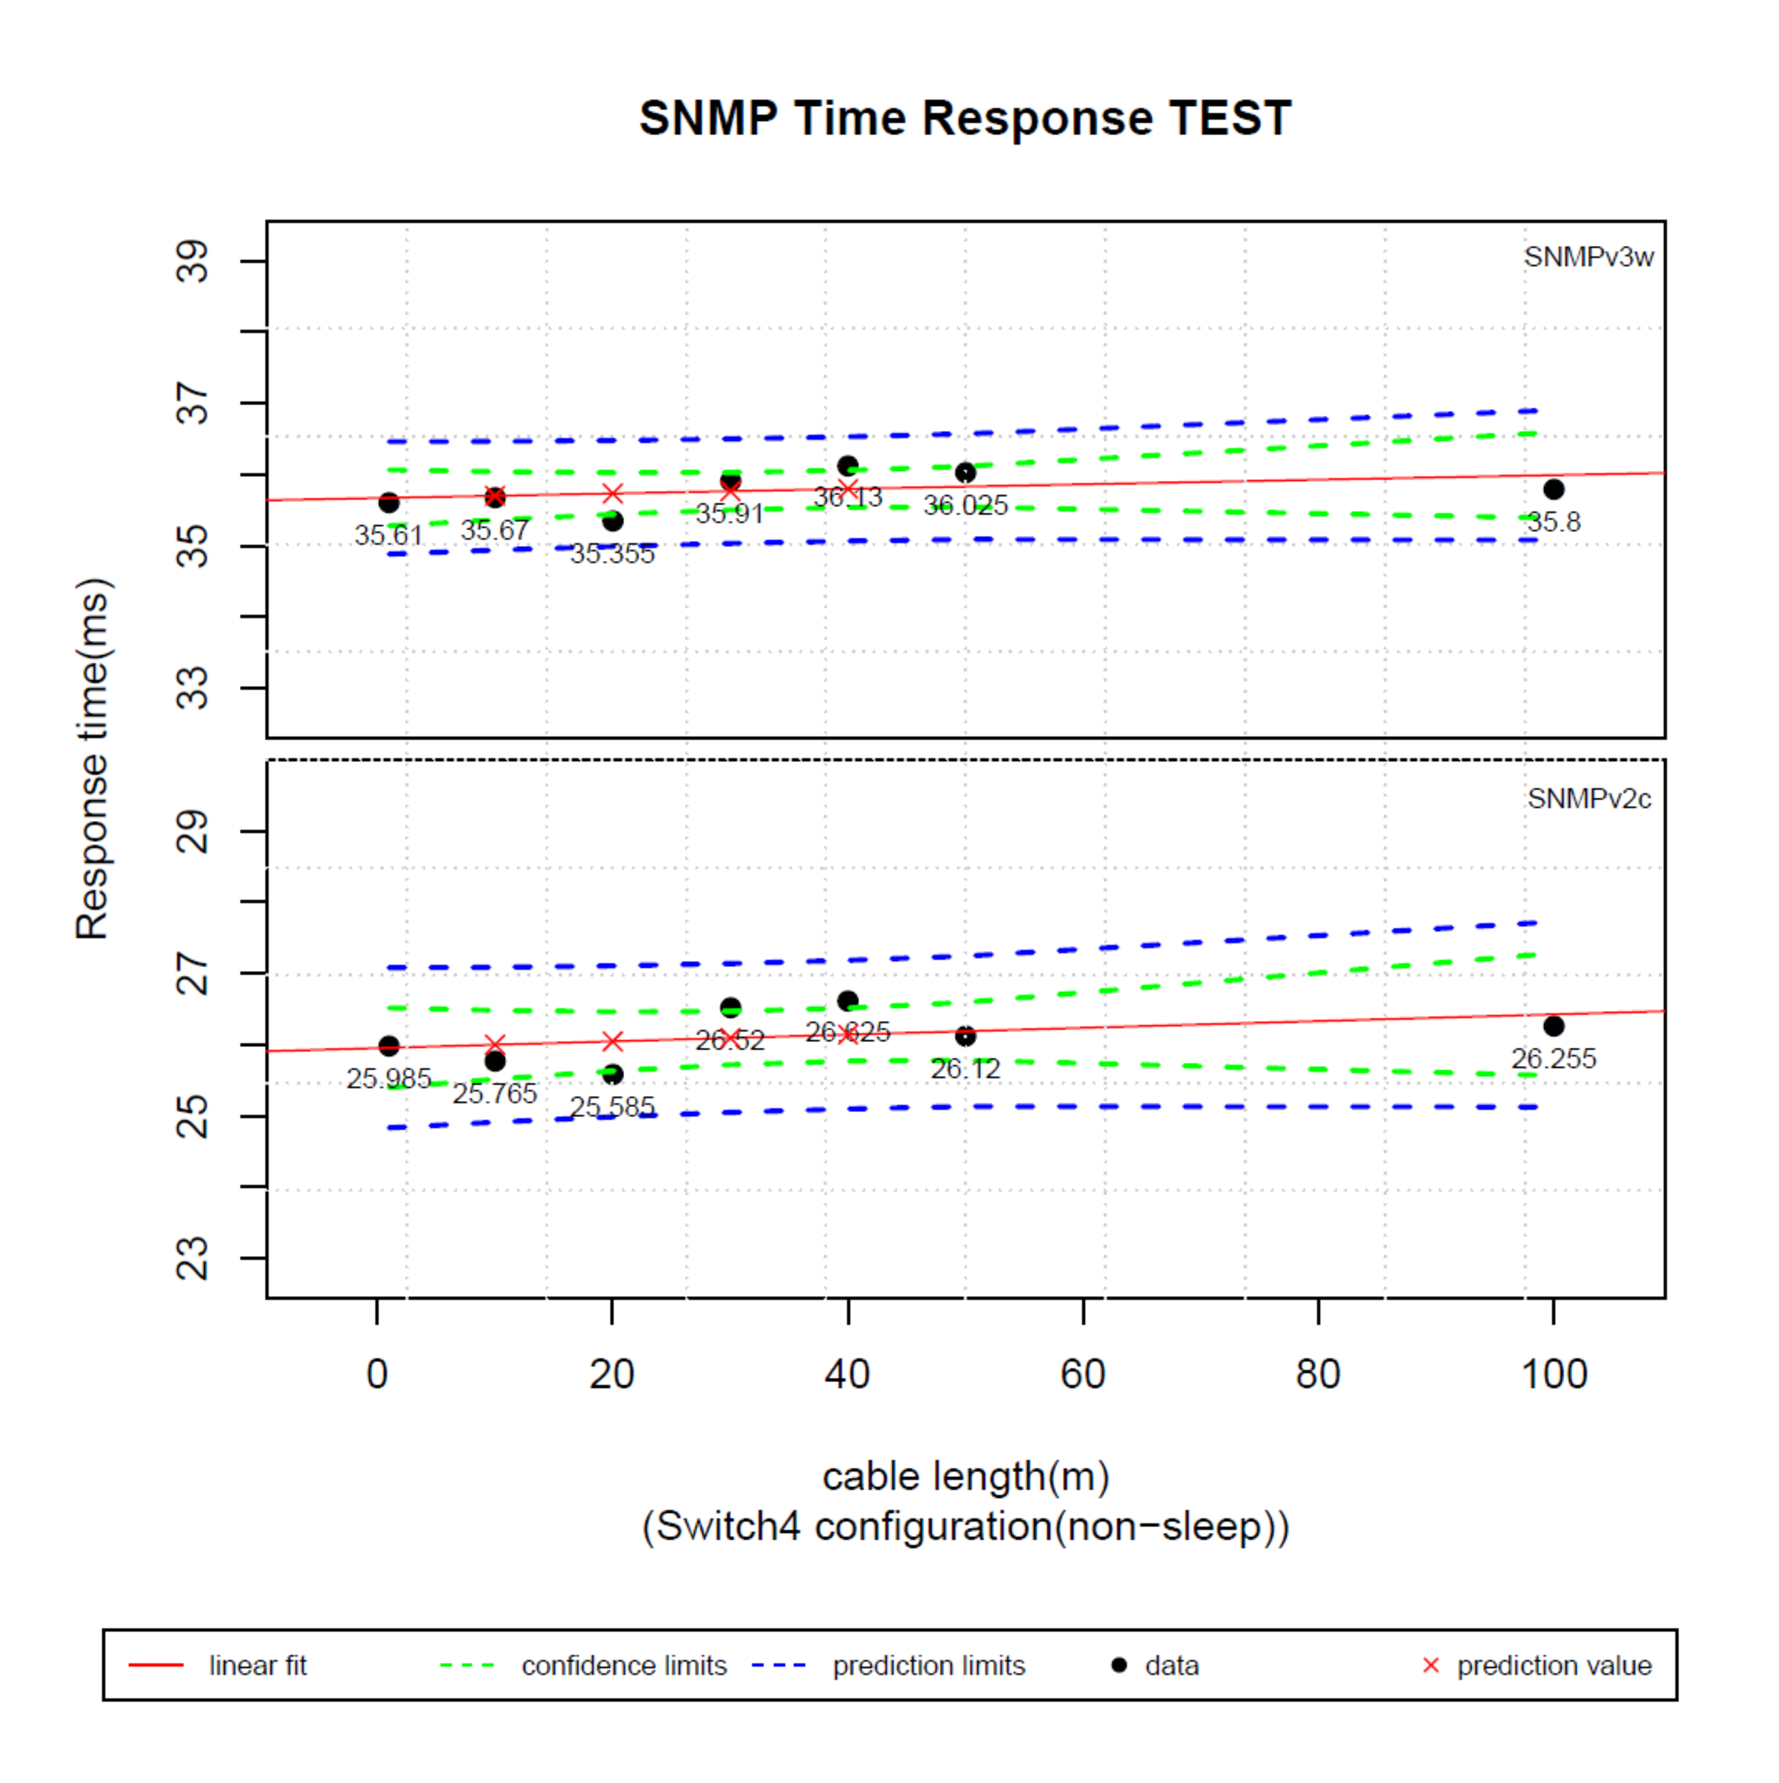
\includegraphics[width=0.5\textwidth]{./images/s4sx.eps}
  \caption{Switch4/Non-Sleep 회귀분석 그래프}
\end{figure}


\begin{table}[!htb]
\begin{center}
\begin{tabular}{c|c|c|c|c}\hline
& \multicolumn{4}{l}{Value} \\ \hline
Independent variable & v1 & v2c & v3r & v3w \\ \hline\hline
p-value& 0.41 & 0.36 & 0.42 & 0.38 \\ \hline
F-value& 0.81 & 1.01 & 0.78 & 0.95 \\ \hline
$  R^2  $ & 0.14 & 0.17 & 0.13 & 0.16 \\\hline
$ Adjusted R^2 $ & -0.03 & 0.00245 & -0.04 & -0.00774 \\\hline 
\multicolumn{5}{l}{*p < 0.05} \\ \hline
\end{tabular}
\caption{Switch4/Non-Sleep 회귀분석 결과}
\end{center}
\end{table} 

\begin{table}[!htb]
\begin{center}
\begin{tabular}{c|c}\hline
 & 회귀식  \\ \hline\hline
v1 &  $ t=0.005327\alpha + 26.020410 $  \\ 
v2c & $ t=0.004839\alpha + 25.946474 $ \\ 
v3r & $ t=0.003153\alpha + 35.722665 $ \\ 
v3w & $ t=0.003223\alpha + 35.668707 $  \\ \hline
\end{tabular}
\caption{Switch4/Non-Sleep 버전별 회귀식}
\end{center}
\end{table} 


\clearpage
\paragraph{2) Sleep 1s}
    
\begin{figure}[h!]
  \centering
  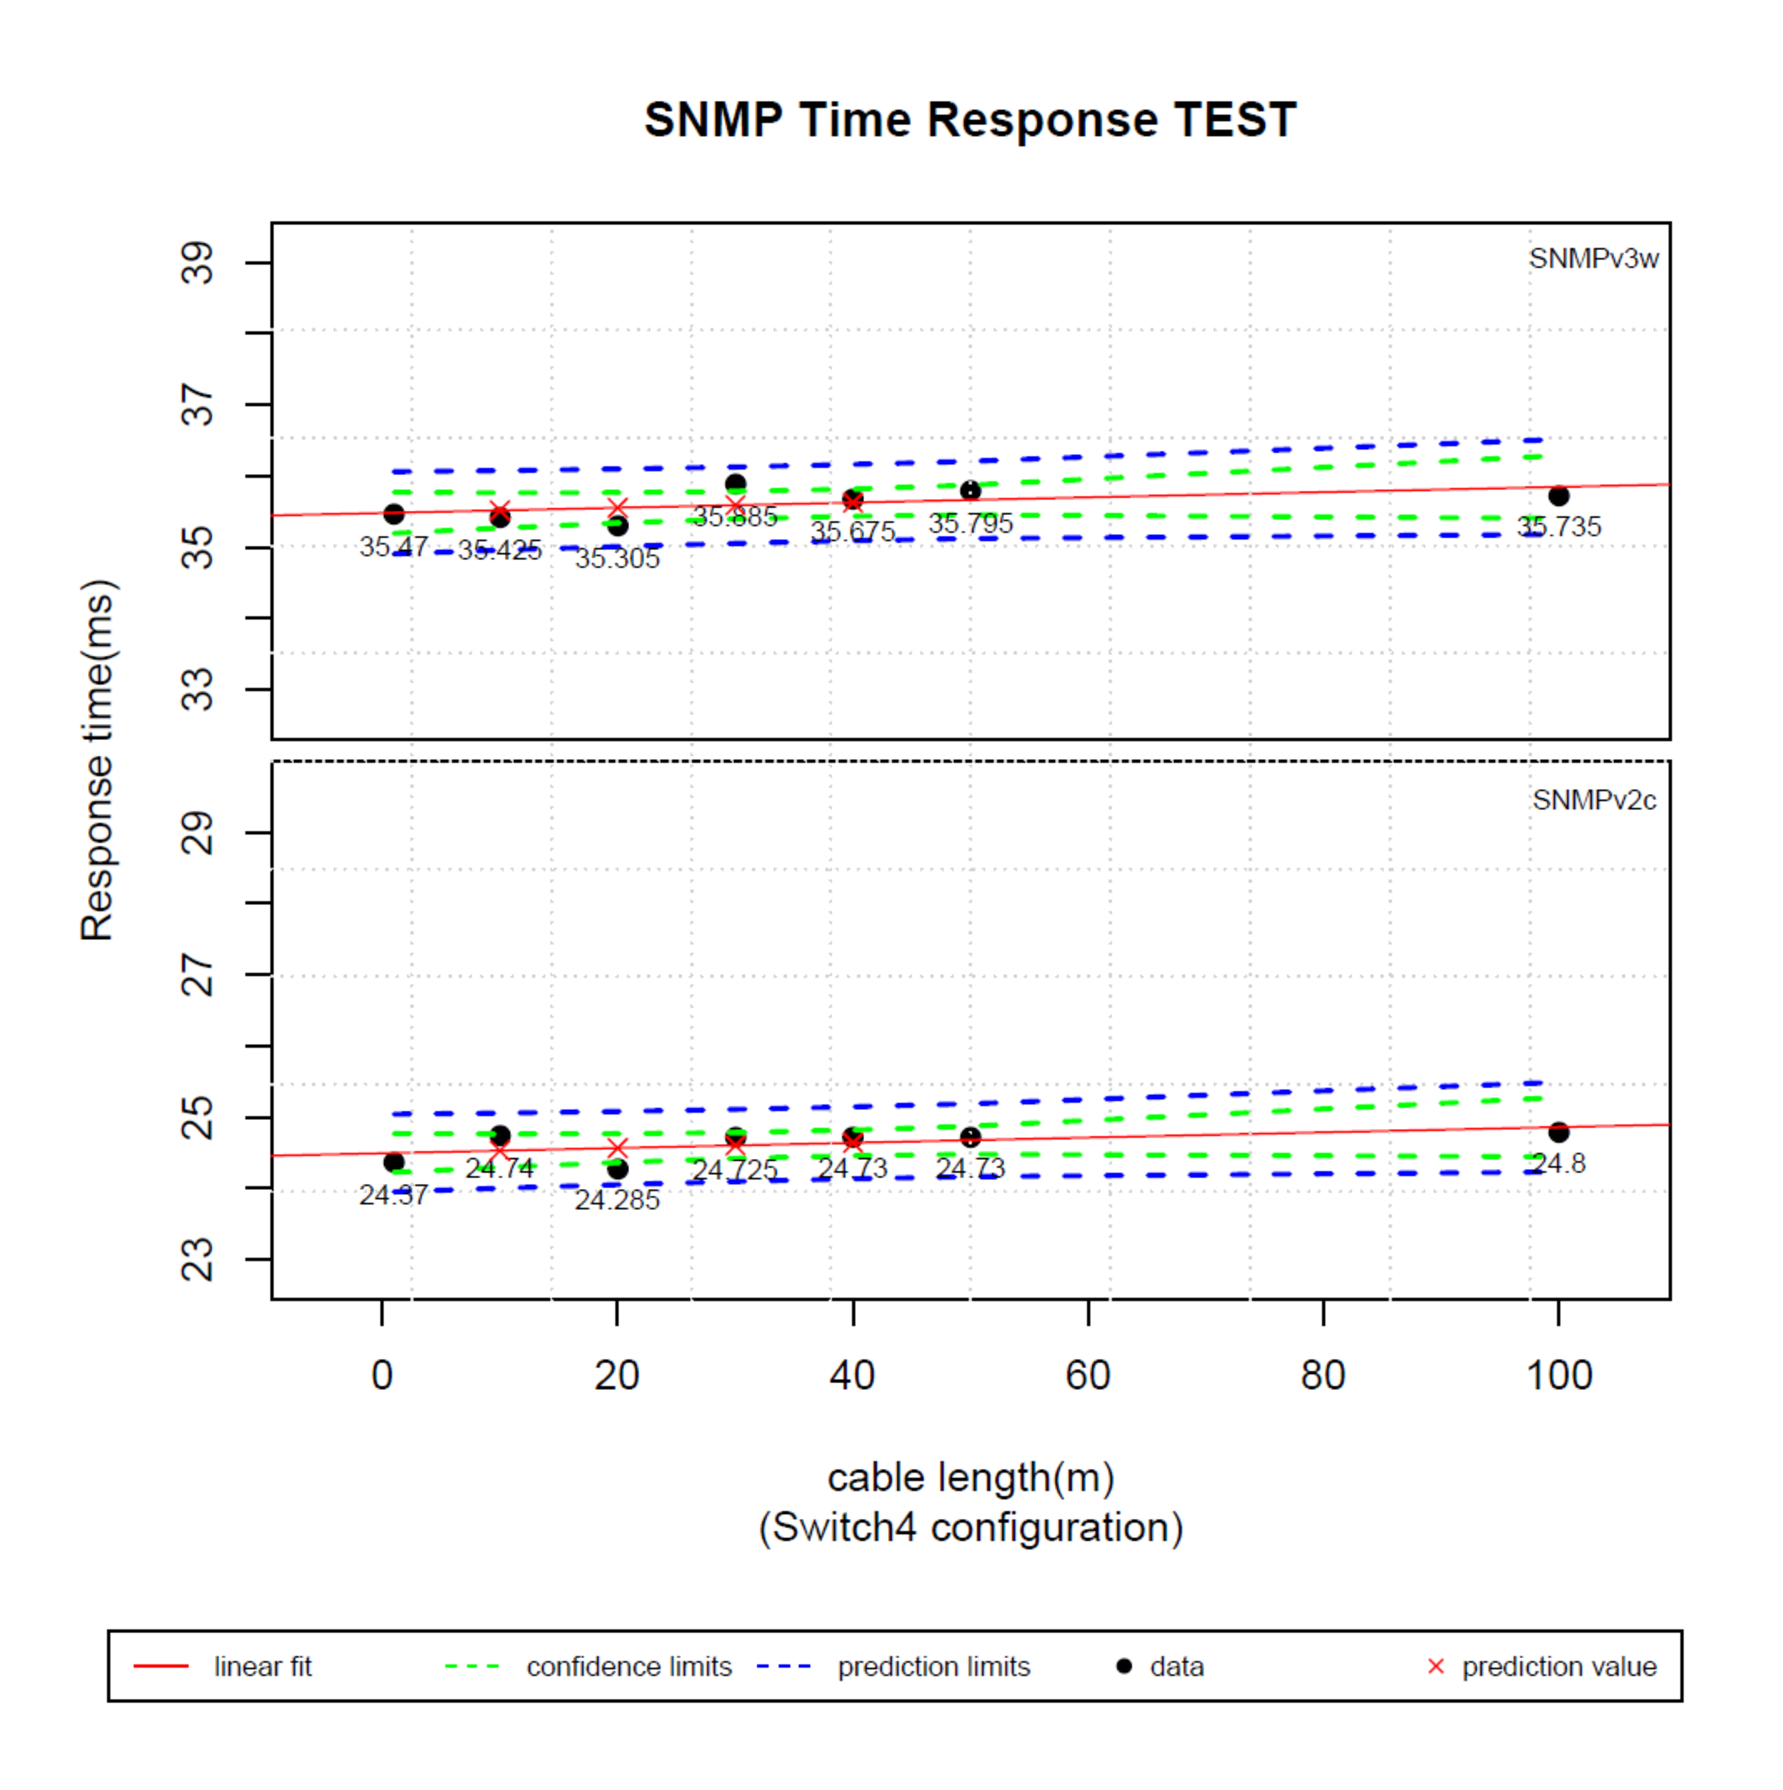
\includegraphics[width=0.5 \textwidth]{./images/s4s1.eps}
  \caption{Switch4/Sleep 1s 회귀분석 그래프}
4\end{figure}


\begin{table}[!htb]
\begin{center}
\begin{tabular}{c|c|c|c|c}\hline
& \multicolumn{4}{l}{Value} \\ \hline
Independent variable & v1 & v2c & v3r & v3w \\ \hline\hline
p-value& 0.000107 & 0.17 & 0.11 & 0.19 \\ \hline
F-value& 122 & 2.59 & 3.70 & 2.30 \\ \hline
$  R^2  $ & 0.96 & 0.34 & 0.43 & 0.32 \\\hline
$ Adjusted R^2 $ & 0.95 & 0.21 & 0.31 & 0.18  \\\hline 
\multicolumn{5}{l}{*p < 0.05} \\ \hline
\end{tabular}
\caption{Switch4/Sleep 1s 회귀분석 결과}
\end{center}
\end{table} 

\begin{table}[!htb]
\begin{center}
\begin{tabular}{c|c}\hline
 & 회귀식  \\ \hline\hline
v1 &  $ t=0.01158\alpha + 24.308871 $  \\ 
v2c & $ t=0.003688\alpha + 24.492049 $ \\ 
v3r & $ t=0.004838\alpha + 35.476529 $ \\ 
v3w & $ t=0.003736\alpha + 35.480340 $  \\ \hline
\end{tabular}
\caption{Switch4/Sleep 1s 버전별 회귀식}
\end{center}
\end{table} 

\subsubsection{A.2.2.5 Switch 5}
\paragraph{1) Non-Sleep}
    
\begin{figure}[h!]
  \centering
  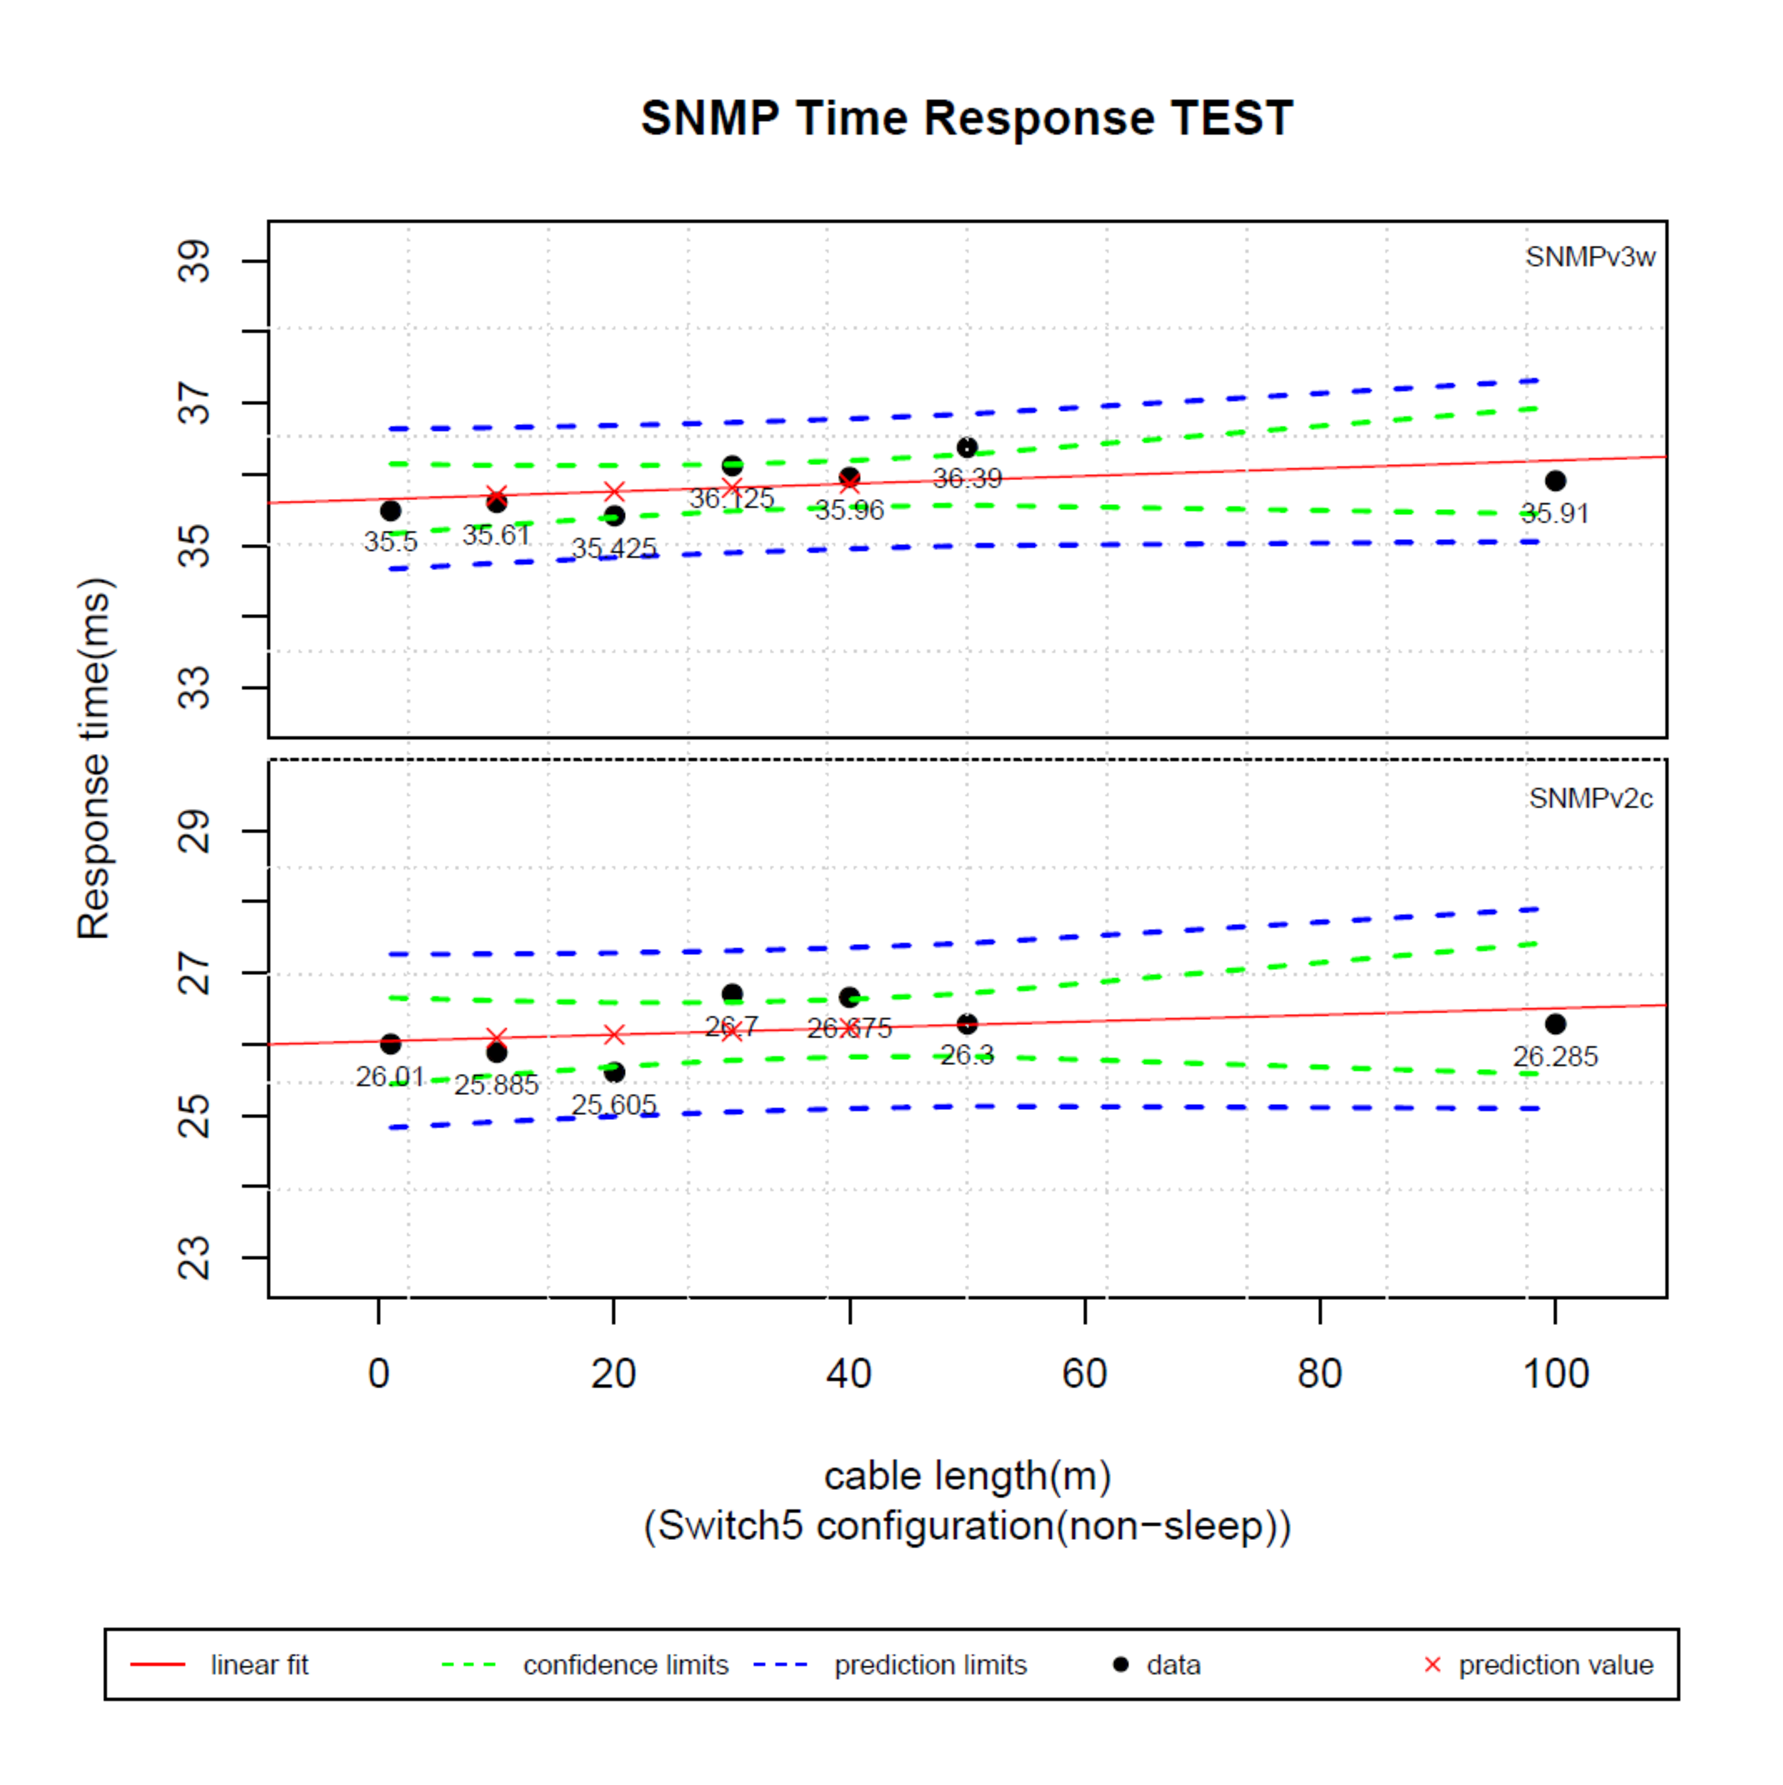
\includegraphics[width=0.5\textwidth]{./images/s5sx.eps}
  \caption{Switch5/Non-Sleep 회귀분석 그래프}
\end{figure}


\begin{table}[!htb]
\begin{center}
\begin{tabular}{c|c|c|c|c}\hline
& \multicolumn{4}{l}{Value} \\ \hline
Independent variable & v1 & v2c & v3r & v3w \\ \hline\hline
p-value& 0.62 & 0.41 & 0.16 & 0.24 \\ \hline
F-value& 0.29 & 0.83 & 2.70 & 1.76 \\ \hline
$  R^2  $ & 0.05 & 0.14 & 0.350 & 0.26 \\\hline
$ Adjusted R^2 $ & -0.14 & -0.03 & 0.220 & 0.11 \\\hline 
\multicolumn{5}{l}{*p < 0.05} \\ \hline
\end{tabular}
\caption{Switch5/Non-Sleep 회귀분석 결과}
\end{center}
\end{table} 


\begin{table}[!htb]
\begin{center}
\begin{tabular}{c|c}\hline
 & 회귀식  \\ \hline\hline
v1 &  $ t=0.004161\alpha + 26.087957 $  \\ 
v2c & $ t=0.004617\alpha + 26.041576 $ \\ 
v3r & $ t=0.006125\alpha + 35.610363 $ \\ 
v3w & $ t=0.005474\alpha + 35.648011 $  \\ \hline
\end{tabular}
\caption{Switch5/Non-Sleep 버전별 회귀식}
\end{center}
\end{table} 


\clearpage
\paragraph{2) Sleep 1s}
    
\begin{figure}[h!]
  \centering
  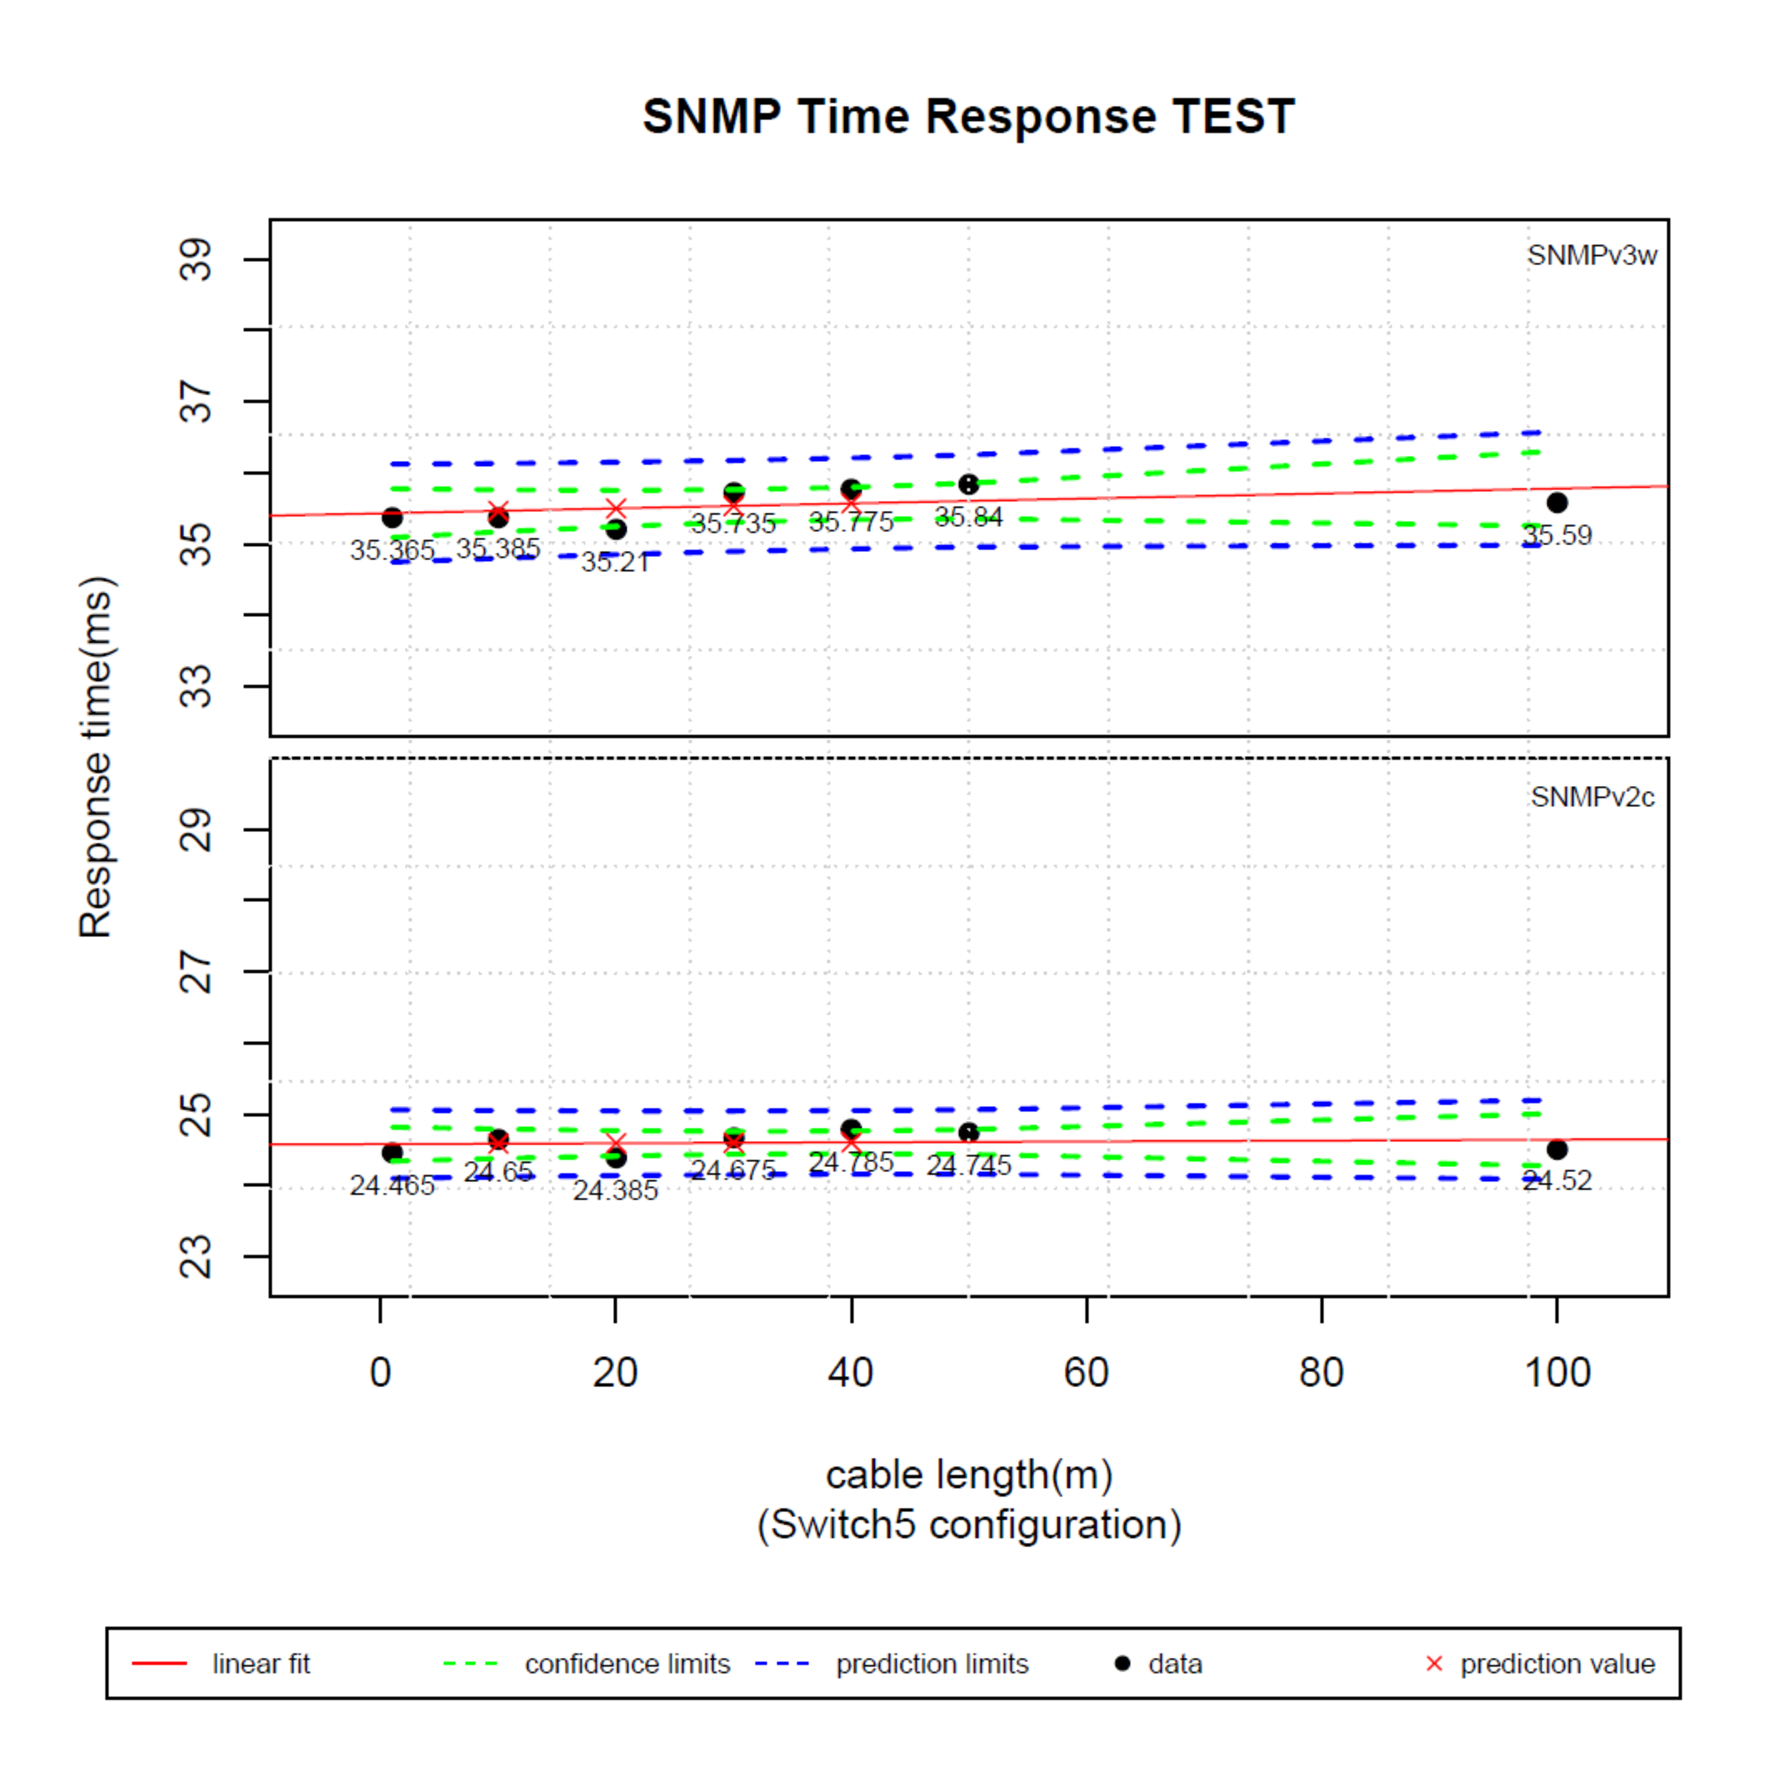
\includegraphics[width=0.5 \textwidth]{./images/s5s1.eps}
  \caption{Switch5/Sleep 1s 회귀분석 그래프}
4\end{figure}


\begin{table}[!htb]
\begin{center}
\begin{tabular}{c|c|c|c|c}\hline
& \multicolumn{4}{l}{Value} \\ \hline
Independent variable & v1 & v2c & v3r & v3w \\ \hline\hline
p-value& 0.75 & 0.77 & 0.60 & 0.28 \\ \hline
F-value& 0.11 & 0.10 & 0.32 & 1.47 \\ \hline
$  R^2  $ & 0.02 & 0.02 & 0.06 & 0.23 \\\hline
$ Adjusted R^2 $ &-0.17 & -0.18 & -0.13 & 0.07 \\\hline 
\multicolumn{5}{l}{*p < 0.05} \\ \hline
\end{tabular}
\caption{Switch5/Sleep 1s 회귀분석 결과}
\end{center}
\end{table} 


\begin{table}[!htb]
\begin{center}
\begin{tabular}{c|c}\hline
 & 회귀식  \\ \hline\hline
v1 &  $ t=-0.0009361\alpha + 24.6478530$  \\ 
v2c & $ t=0.6.463e^-04\alpha + 2.458e^+01$ \\ 
v3r & $ t=0.001473\alpha + 35.501476 $ \\ 
v3w & $ t=0.003525\alpha + 35.430737 $  \\ \hline
\end{tabular}
\caption{Switch5/Sleep 1s 버전별 회귀식}
\end{center}
\end{table} 

\clearpage
\subsection{A.2.3 다중회귀분석결과}
\subsubsection{A.2.3.1 SNMPv1}
\centering 회귀식 $ t=4.402e^-06\alpha_1 + 3.536e^-05\alpha_2 + 2.431e^-02$ 
    
\begin{figure}[h!]
  \centering
  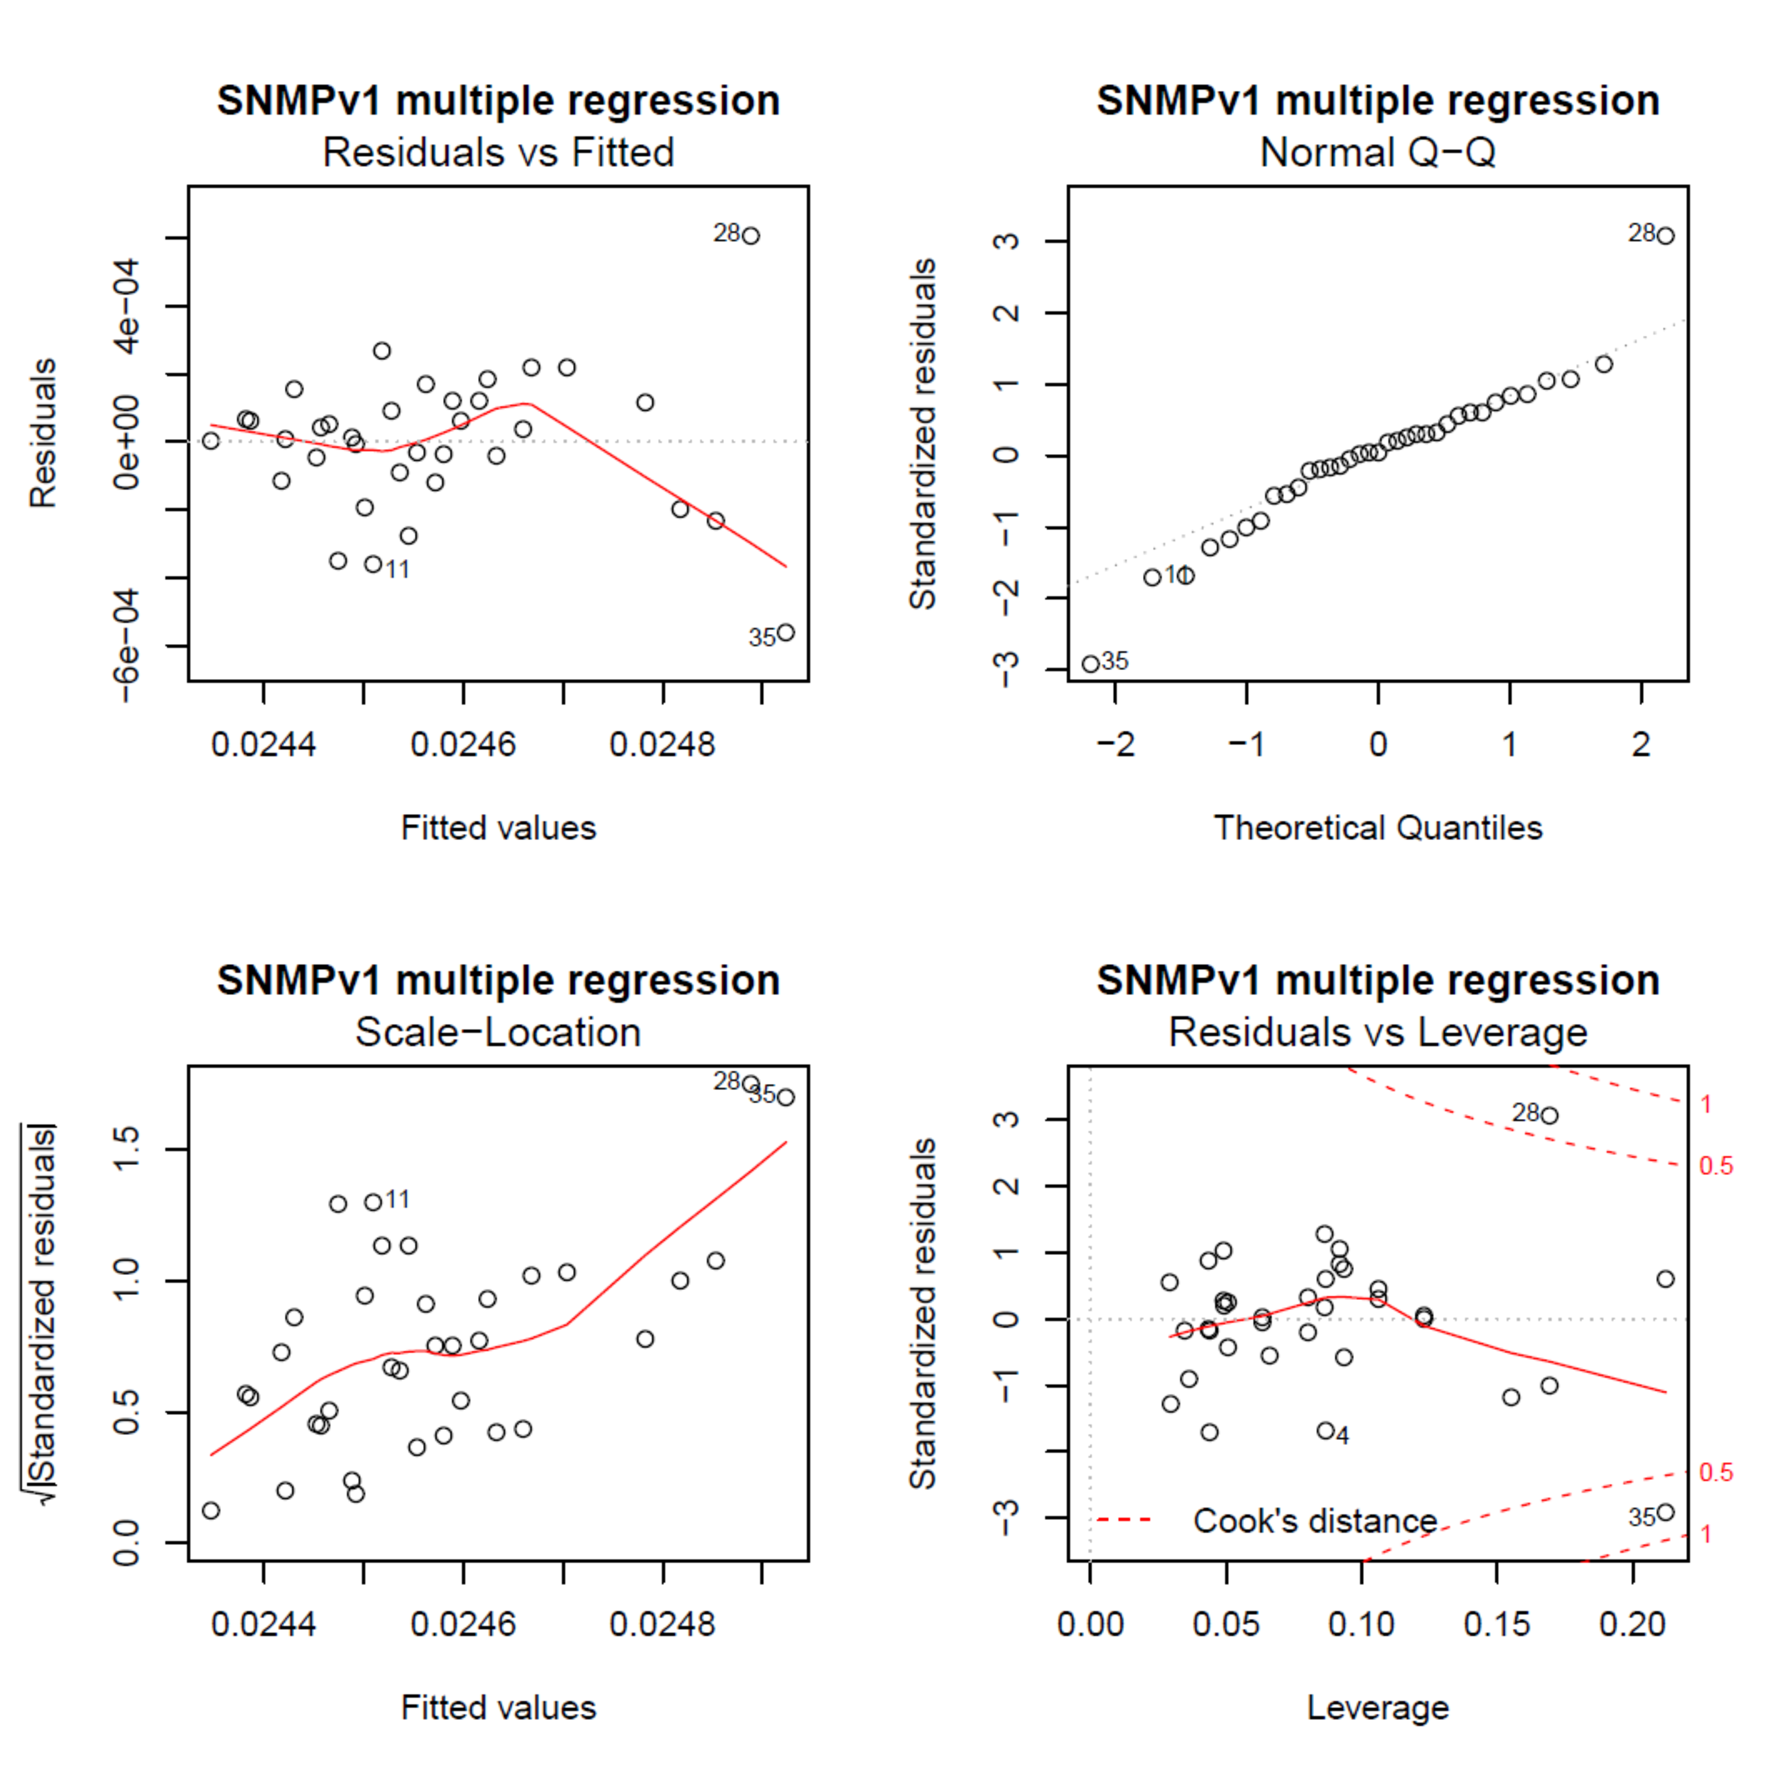
\includegraphics[width=0.8\textwidth]{./images/v1.eps}
  \caption{다중회귀분석 그래프 (SNMPv1)}
\end{figure}

\begin{table}[!h]
\begin{center}
\begin{tabular}{c|c}\hline
Independent variable & Value  \\ \hline\hline
p-value &  0.001964\\ 
F-value &  7.621\\ 
$  R^2  $ &  0.3226\\ 
$ Adjusted R^2 $ & 0.2803 \\ \hline
\multicolumn{2}{l}{*p < 0.05} \\ \hline\hline
\end{tabular}
\caption{다중회귀분석 결과 (SNMPv1)}
\end{center}
\end{table} 
\clearpage


\subsubsection{A.2.3.2 SNMPv2c}
\centering 회귀식 $ t=3.782e^-06\alpha_1 + 1.664e^-05\alpha_2 + 2.440e^-02$ 
    
\begin{figure}[h!]
  \centering
  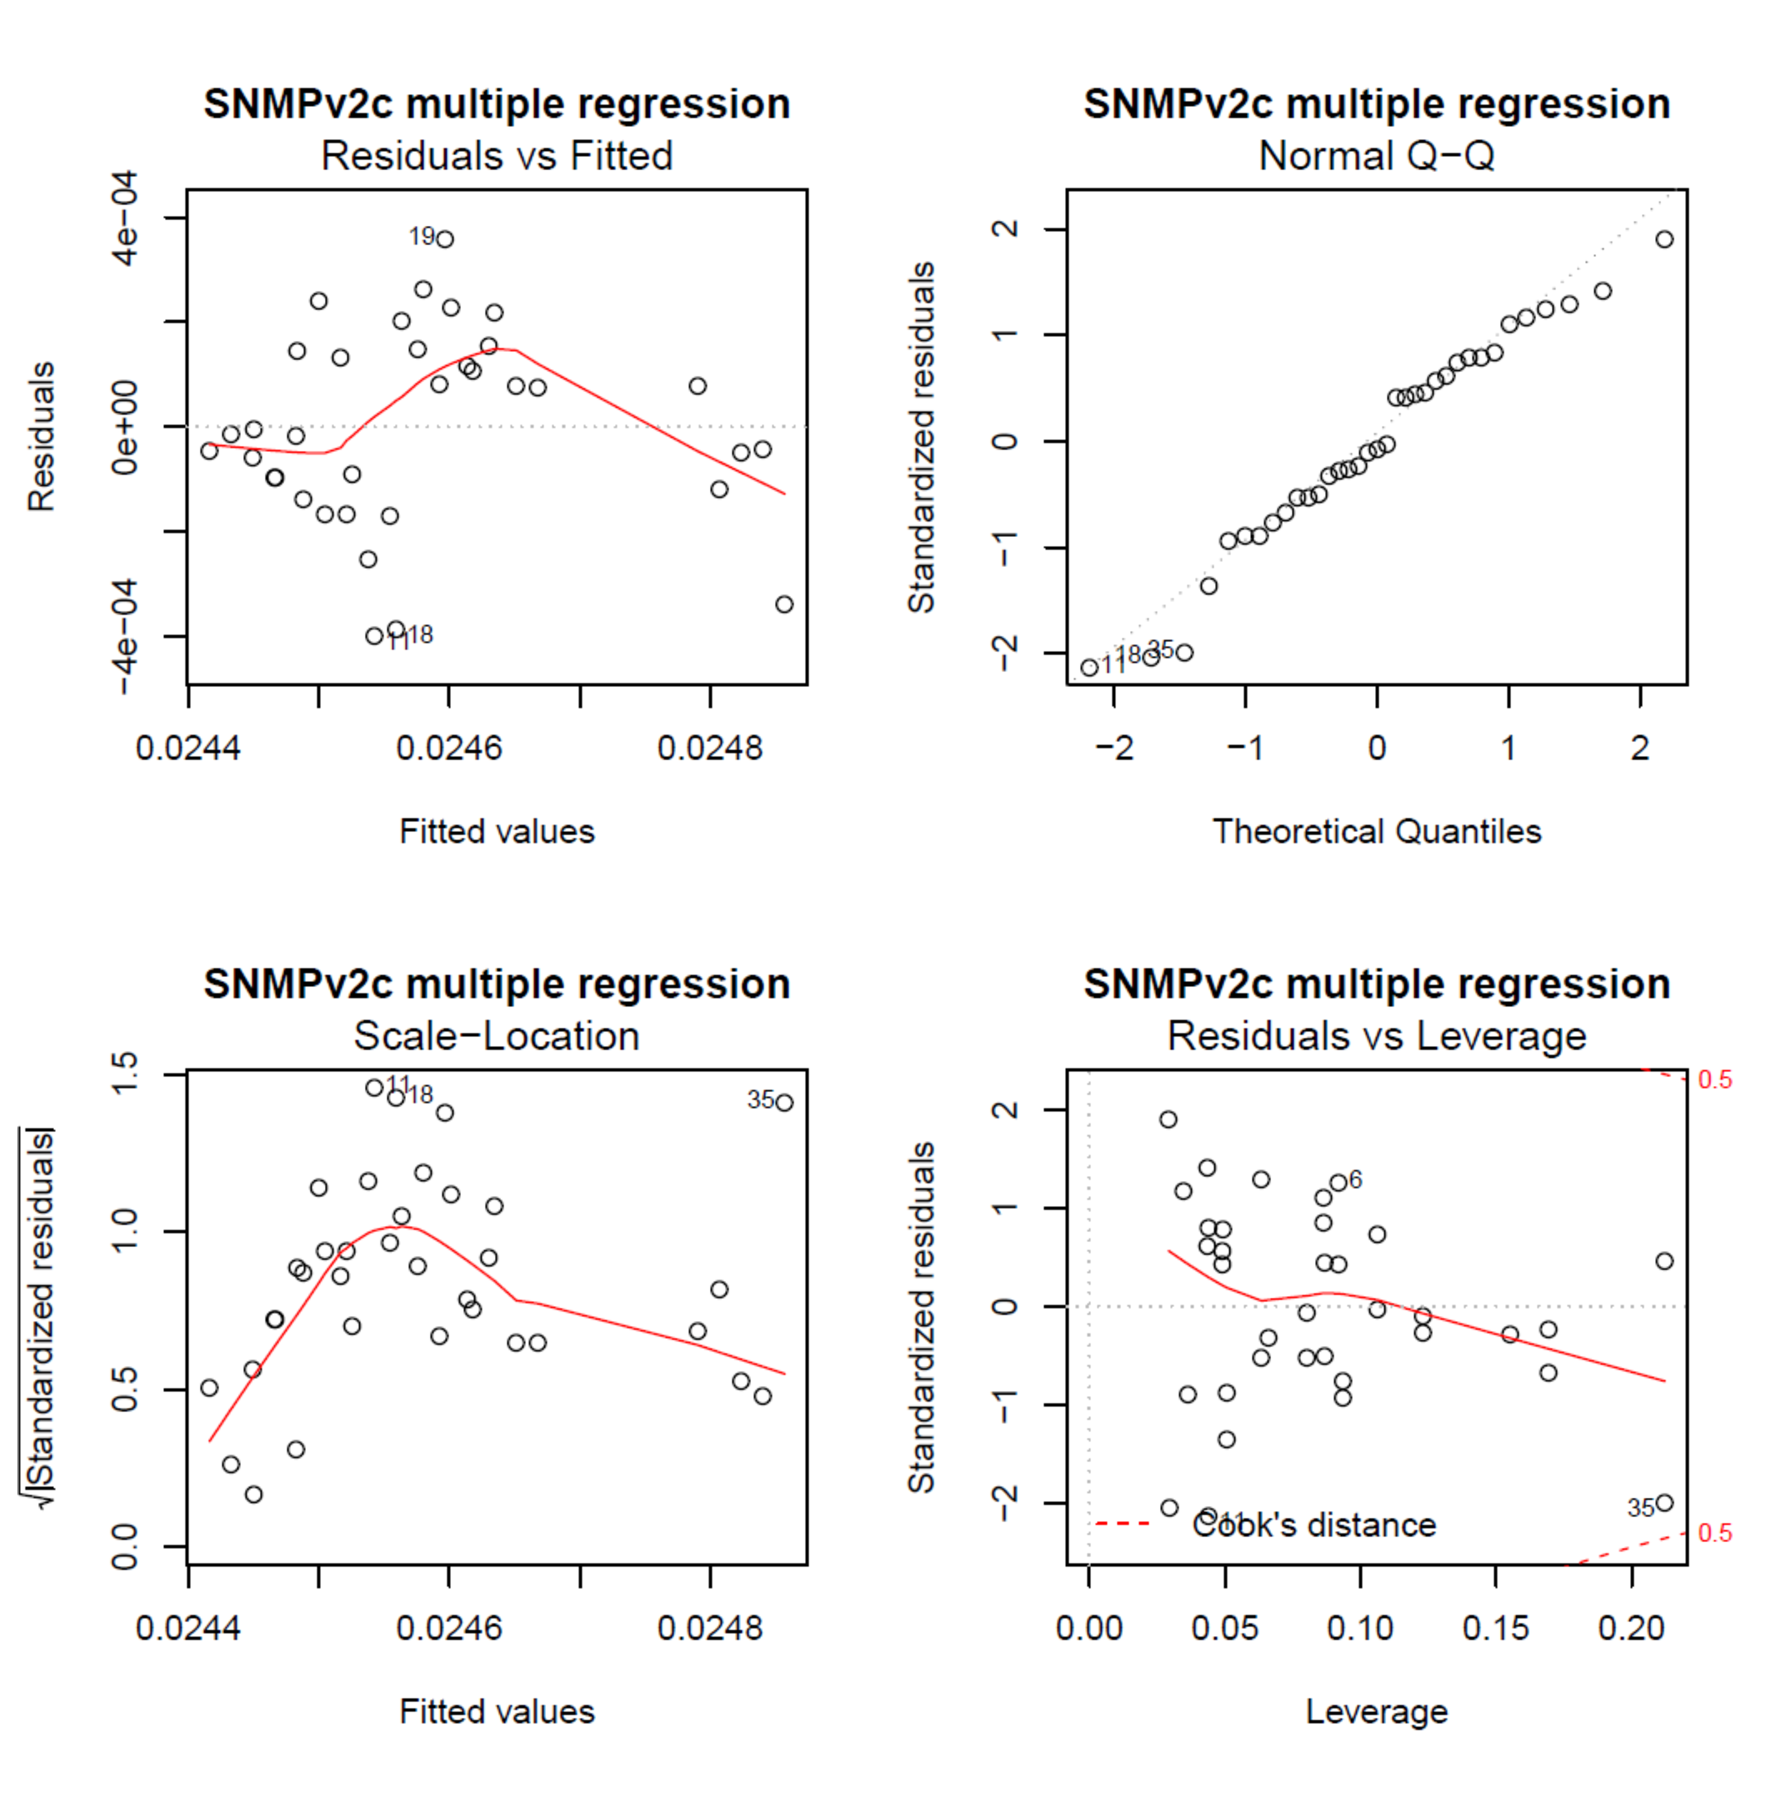
\includegraphics[width=0.8\textwidth]{./images/v2c.eps}
  \caption{다중회귀분석 그래프 (SNMPv2c)}
\end{figure}

\begin{table}[!h]
\begin{center}
\begin{tabular}{c|c}\hline
Independent variable & Value  \\ \hline\hline
p-value &  0.003907\\ 
F-value &  6.627\\ 
$  R^2  $ &  0.02929\\ 
$ Adjusted R^2 $ & 0.2487 \\ \hline
\multicolumn{2}{l}{*p < 0.05} \\ \hline\hline
\end{tabular}
\caption{다중회귀분석 결과 (SNMPv2c)}
\end{center}
\end{table} 
\clearpage


\subsubsection{A.2.3.3 SNMPv3r}
\centering 회귀식 $ t=4.056e^-06\alpha_1 + 1.479e^-05\alpha_2 + 3.318e^-02$ 
    
\begin{figure}[h!]
  \centering
  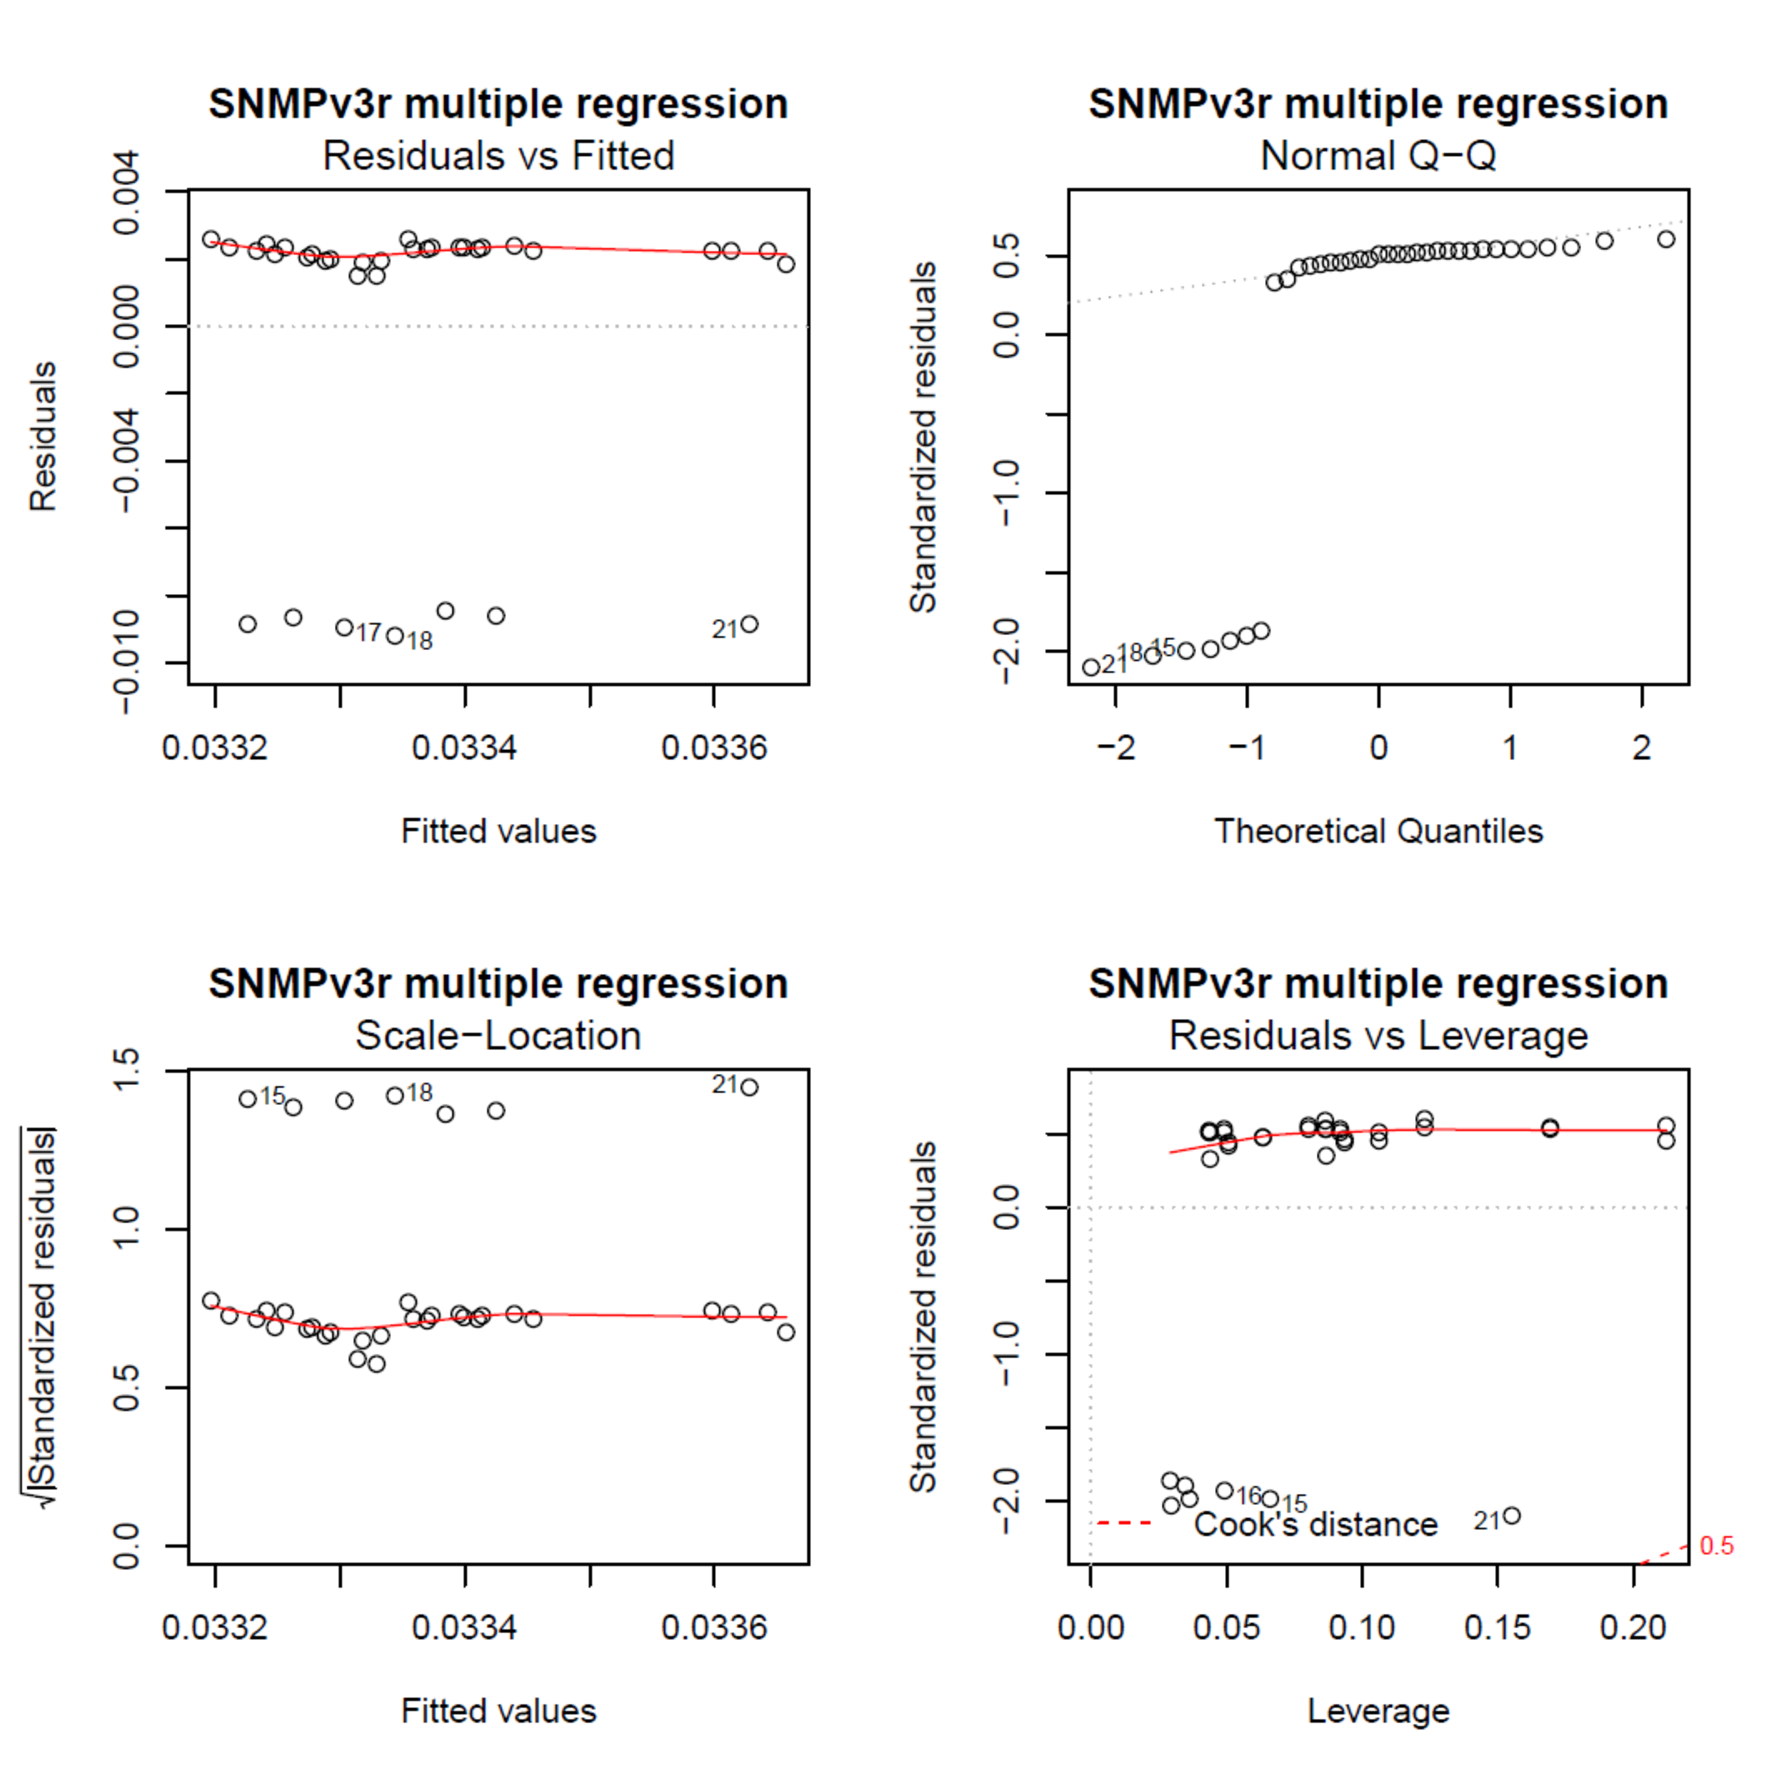
\includegraphics[width=0.8\textwidth]{./images/v3r.eps}
  \caption{다중회귀분석 그래프 (SNMPv3r)}
\end{figure}

\begin{table}[!h]
\begin{center}
\begin{tabular}{c|c}\hline
Independent variable & Value  \\ \hline\hline
p-value &  0.9871\\ 
F-value &  0.01301\\ 
$  R^2  $ &  0.0008124\\ 
$ Adjusted R^2 $ & -0.06164 \\ \hline
\multicolumn{2}{l}{*p < 0.05} \\ \hline\hline
\end{tabular}
\caption{다중회귀분석 결과 (SNMPv3r)}
\end{center}
\end{table} 
\clearpage

\subsubsection{A.2.3.4 SNMPv3w}
\centering 회귀식 $ t=4.416e^-06\alpha_1 - 4.214^-06\alpha_2 + 3.546e^-02$ 
    
\begin{figure}[h!]
  \centering
  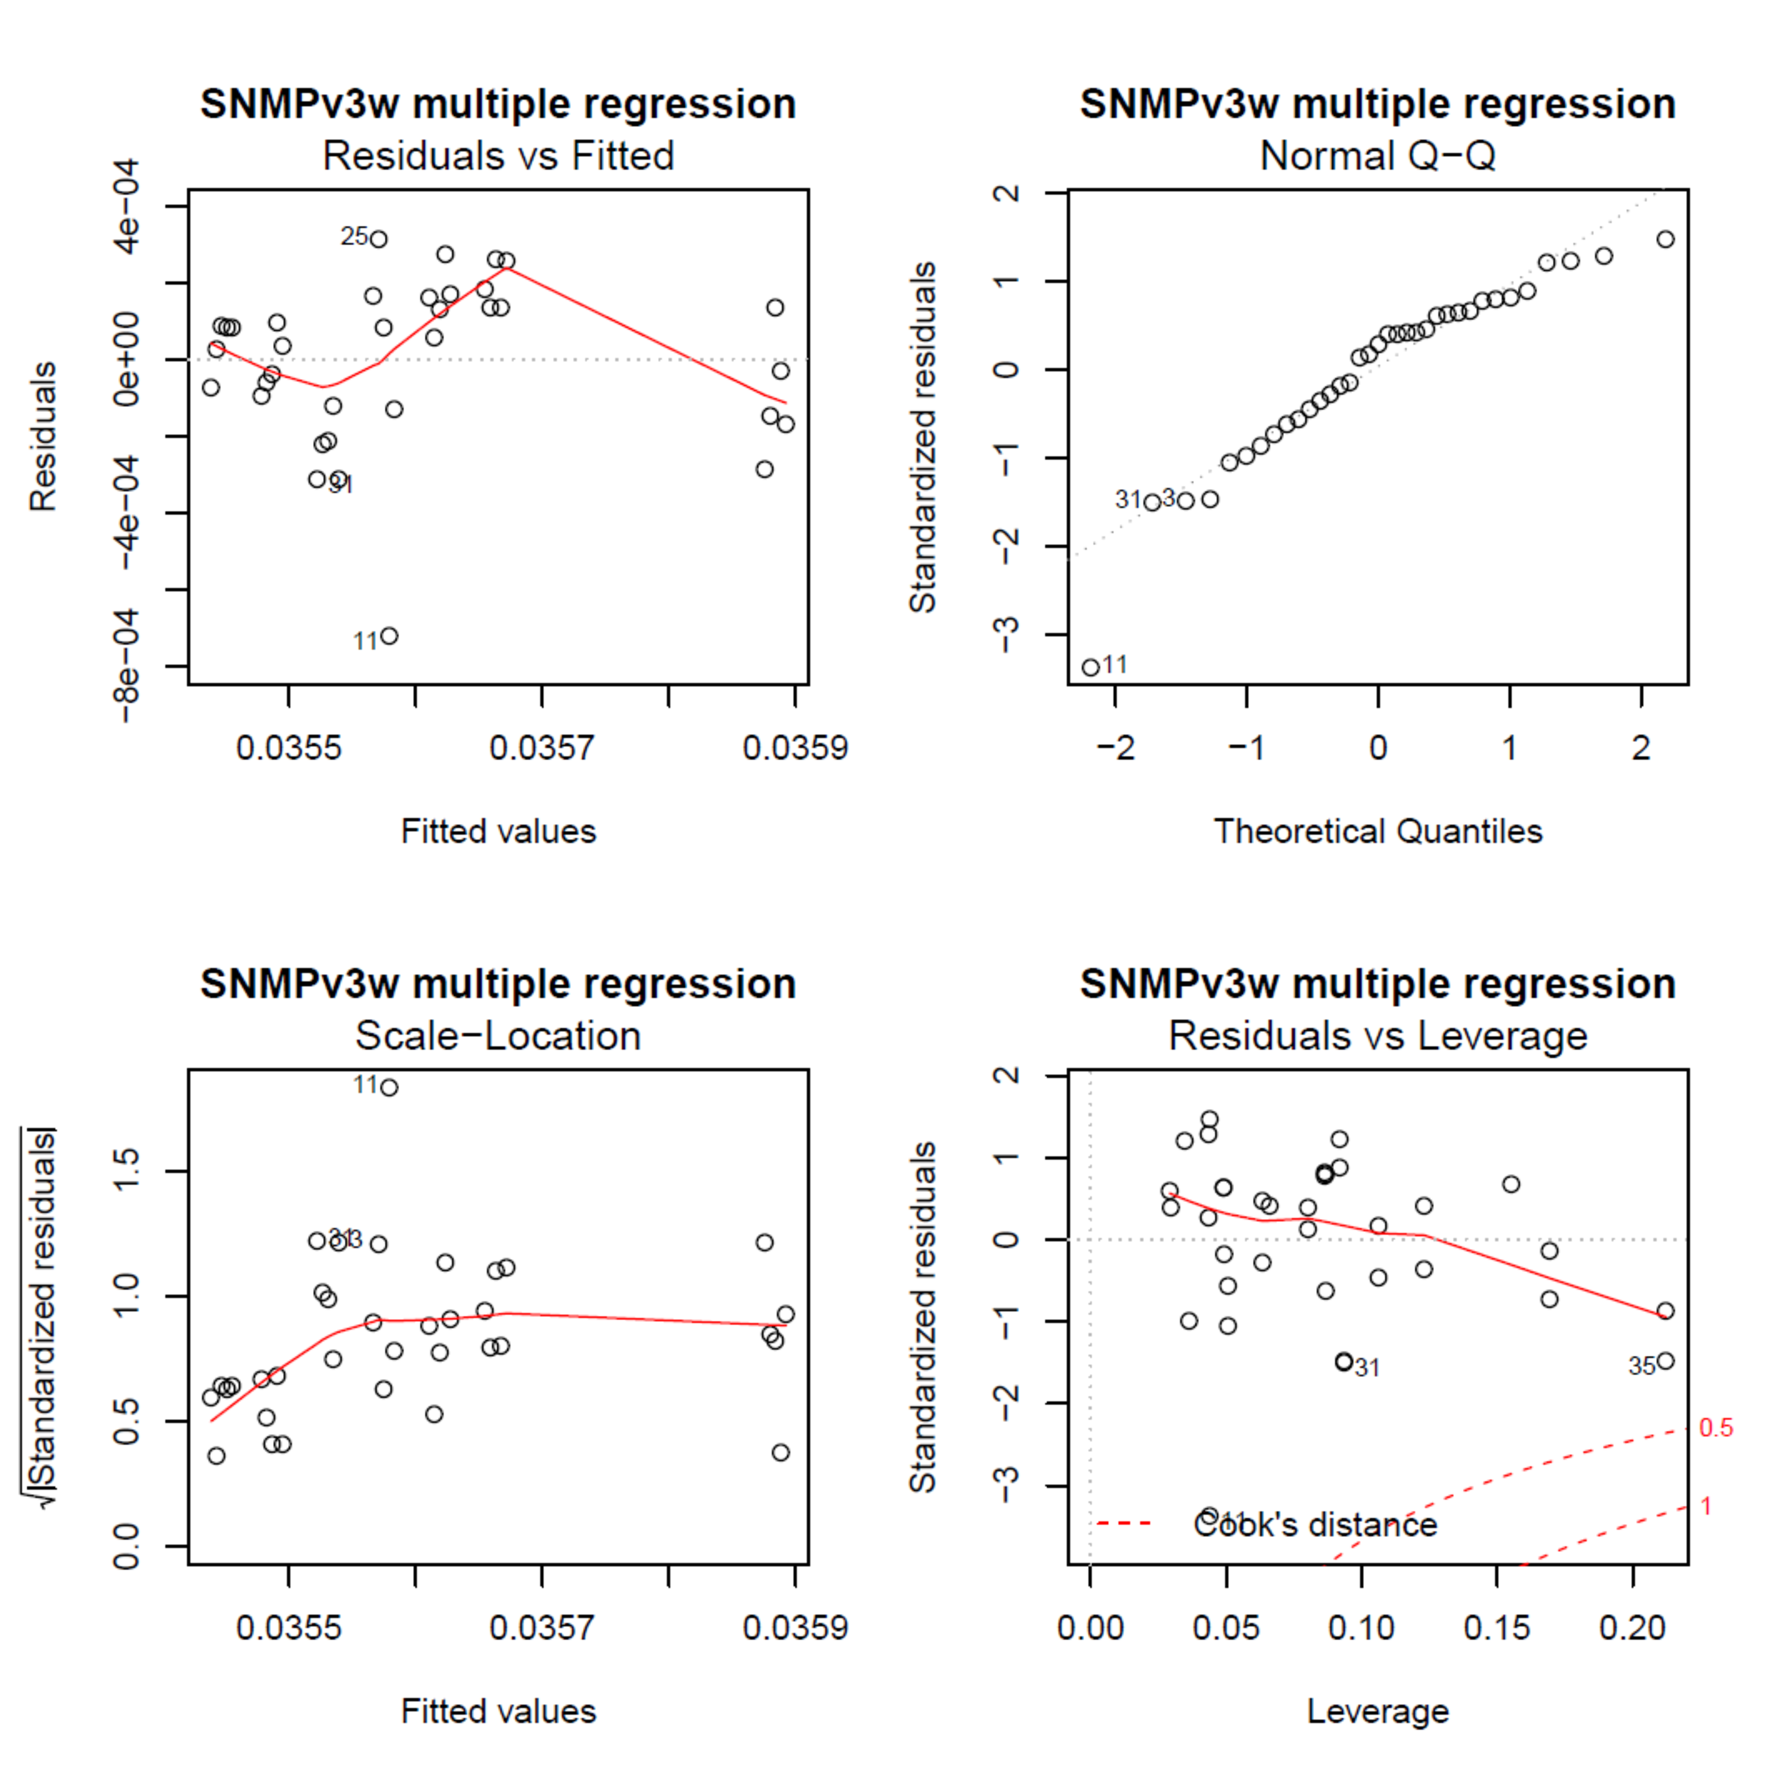
\includegraphics[width=0.8\textwidth]{./images/v3w.eps}
  \caption{다중회귀분석 그래프 (SNMPv3w)}
\end{figure}

\begin{table}[!h]
\begin{center}
\begin{tabular}{c|c}\hline
Independent variable & Value  \\ \hline\hline
p-value &  0.003894\\ 
F-value &  6.632\\ 
$  R^2  $ &  0.293\\ 
$ Adjusted R^2 $ & 0.2488 \\ \hline
\multicolumn{2}{l}{*p < 0.05} \\ \hline\hline
\end{tabular}
\caption{다중회귀분석 결과 (SNMPv3w)}
\end{center}
\end{table} 
\clearpage
\bibliographystyle{unsrtnat}
\bibliography{./refs}

\end{document}
